\chapter{AccessibleHub: Transforming mobile accessibility guidelines into code}
\label{chap:accessibility-toolkit}

\chapterintroline{
    This chapter introduces an accessibility learning toolkit for mobile developers. Building upon prior research, it provides a practical guide to implementing accessible mobile applications, particularly in Flutter. \textit{AccessibleHub}, a \gls{reactnative} toolkit, offers interactive examples and component-level guidance, comparing React Native and \gls{flutter}. Grounded in \gls{wcagg} principles, AccessibleHub aims to bridge the gap between accessibility guidelines and real-world application.
}

\section{Introduction}
\label{sec:intro}

\subsection{Challenges in implementing accessibility guidelines}

The importance of mobile app accessibility extends beyond mere compliance with legal regulations. Ensuring equal access to digital content and services is not only an ethical obligation but also a smart business decision. By prioritizing accessibility, app developers and companies can tap into a larger user base, improve user satisfaction, and demonstrate their commitment to social responsibility.
Despite the clear benefits and moral imperatives of mobile app accessibility, many developers still struggle to effectively implement accessibility guidelines in their projects. The \acrshort{wcagacr}, developed by the \gls{w3cg}, serve as the international standard for digital accessibility. However, translating these guidelines into practical implementation can be a challenging task, particularly starting from pure formal guidelines into everyday code. \\

One of the primary challenges lies in the complexity of the guidelines themselves. WCAG encompasses a wide range of \textit{success criteria}, organized under four main general \textit{principles}: perceivable, operable, understandable, and robust. Each principle contains multiple guidelines, and each guideline has several success criteria at different levels of \textit{conformance} (A, AA, AAA). Navigating this intricate web of requirements and understanding how to apply them to specific mobile app components can be overwhelming for developers, especially those new to accessibility. 
Moreover, the practical implementation of accessibility guidelines often varies across different platforms and frameworks. \textit{iOS} and \textit{Android}, the two dominant mobile operating systems, have their own unique accessibility \textit{API}s, tools, and best practices. Cross-platform frameworks like React Native and Flutter add another layer of complexity, as developers must ensure that their accessibility implementations are compatible with the underlying platform-specific mechanisms. \\ 

Furthermore, there is often a lack of clear, practical examples and guidance on how to implement accessibility features in real-world mobile app projects. While the \textit{WCAG} provides a solid foundation, it is primarily focused on web content and may not always directly address the unique challenges and interaction patterns of mobile apps. Developers often struggle to bridge the gap between the theoretical guidelines and the specific implementation details required for their projects.

\subsection{The need for practical developer education}

To address these challenges and bridge the gap between accessibility guidelines and practical implementation, there is a pressing need for developer education resources that focus on real-world, hands-on learning experiences. Traditional documentation and guidelines, while valuable, often fall short in providing the level of detail and interactivity needed to effectively guide developers through the accessibility implementation process.
This is where the concept of an \textit{accessibility learning toolkit} comes into play. An accessibility toolkit is designed to serve as a comprehensive, interactive resource that empowers developers to create accessible mobile applications by providing:

\begin{enumerate}
    \item Clear explanations of \acrshort{wcagacr} guidelines and their applicability to mobile apps;
    
    \item Step-by-step implementation guidance for common mobile app components and interaction patterns;
    
    \item Practical code examples and tutorials that demonstrate best practices;
    
    \item Hands-on exercises and challenges to reinforce learning and build confidence;
    
    \item Tools and techniques for testing and validating the accessibility of mobile apps.
\end{enumerate}

The primary goal of an accessibility learning toolkit is to bridge the gap between the theoretical knowledge of accessibility guidelines and the practical skills needed to implement them effectively in real-world projects. 
The toolkit should cater to developers at various levels of expertise, from beginners who are new to accessibility concepts to experienced professionals seeking to deepen their knowledge and stay up-to-date with the latest best practices. By providing a comprehensive, hands-on learning resource, the accessibility toolkit can play a crucial role in promoting a culture of inclusive design and development within the mobile app industry. \\

Current research, including Budai's work on Flutter accessibility testing, has primarily focused on end-user validation and testing methodologies. However, developers need practical, implementation-focused guidance that bridges multiple frameworks and platforms.
Despite widespread accessibility guidelines and standard, mobile application developers face significant challenges in translating theoretical requirements into practical implementations. This gap between guidelines and implementation is particularly evident in mobile development, where different platforms, screen sizes, and interaction models add complexity to accessibility implementation. Some of the most common challenges include:

\begin{itemize}
    \item Complex testing requirements - developers must validate across multiple devices, \gls{screenreaderg}, and interaction modes;
    
    \item Framework-specific implementations - each platform has unique accessibility \gls{apig}s and requirements;
    
    \item Limited practical examples - most documentation focuses on theoretical guidelines rather than concrete implementation patterns;
    
    \item Performance considerations - accessibility features must be implemented without compromising app performance.
\end{itemize}

Effective developer education in accessibility requires a solid grounding in learning theories that emphasize hands-on, interactive approaches. By integrating established learning theories with technical education principles, it's possible to justify the interactive and practical approach adopted in this toolkit. In doing so, we draw on constructivist and experiential learning models, which have been widely recognized as effective frameworks in technical and developer education.

Constructivist learning theories, pioneered by Piaget \cite{piaget1970science} and Vygotsky \cite{vygotsky1978mind}, posit that learning is an active process in which individuals construct knowledge based on their prior experiences and interactions with the environment. In the context of developer education, this suggests that hands-on learning is more effective than passive instruction \cite{savery2006overview}. By engaging with real-world accessibility challenges and actively experimenting with code implementations, developers can build a deeper understanding of accessibility guidelines and best practices, by having a tool at their disposal easy to use and to navigate. \\

Kolb's \textit{Experiential Learning Theory} \cite{kolb1984experiential} further supports this approach by describing learning as a four-stage cycle: concrete experience, reflective observation, abstract conceptualization, and active experimentation. For developers learning about accessibility, this cycle might involve encountering accessibility issues in their projects, analyzing existing solutions and guidelines, synthesizing their understanding of \acrshort{wcagacr} principles, and applying these principles to their own code. \textit{AccessibleHub} facilitates this learning cycle by providing a structured, interactive environment for developers to engage with accessibility concepts and implementations being organized into different core sections. By aligning with these proven pedagogical approaches, \textit{AccessibleHub} aims to provide an effective and engaging learning experience for developers. Moreover, by fostering a community of practice around accessibility while providing easier access to learning resources, this project encourages ongoing learning and knowledge sharing among developers, promoting the continuous improvement and dissemination of accessibility best practices.

\subsection{Research objectives and methodology}

Building upon previous research into mobile accessibility, this work aims to provide a comprehensive understanding of accessibility implementation across major cross-platform frameworks. While existing research indeed set grounds for both guidelines on accessibility and testing methodologies, there is a critical need to understand how these guidelines translate into practice for developers. 

This research addresses three fundamental questions about accessibility implementation in mobile development frameworks (referring to these ones as \textit{research questions}, following the work in \cite{perinello2024accessibility}:

\begin{itemize}
    \item First, we investigate whether components and widgets provided by frameworks are \textit{accessible by default}, without requiring additional developer intervention. This analysis is crucial for understanding the baseline accessibility support provided by each framework and identifying areas where additional implementation effort may be required;
    
    \item Second, we examine the \textit{feasibility of making non-accessible components accessible} through additional development effort. This involves analyzing the technical capabilities of each framework and identifying the necessary modifications to achieve accessibility compliance;
    
    \item Third, we quantify the \textit{development overhead required to implement accessibility features} when they are not provided by default. This includes measuring additional code requirements, analyzing complexity increases, and evaluating the impact on development workflows.
\end{itemize}

These questions is addressed via the usage of a systematic methodology aiming to address in detail accessibility support in React Native and Flutter, focusing on component implementation patterns and native platform integration. The implementation is comparative, allowing developers to directly implement accessible code examples with different degrees of implementation complexity measured quantitatively (including lines of code, required properties, and additional components needed for accessibility support). Comprehensive testing of implementations is also done using screen readers and other assistive technologies to verify accessibility compliance.

The \textit{goal} is to create an accessible application that serves three key purposes:
\begin{enumerate}
    \item To provide developers with practical, interactive examples of accessibility implementation, able to be copied easily and ported inside of other projects;
    
    \item To compare and contrast accessibility approaches between the main cross-development mobile frameworks in the current mobile landscape;
    
    \item To establish a reusable pattern library that demonstrates engine architecture, widget systems, and native platform integration, while ensuring compliance with current accessibility guidelines and legal requirements.
\end{enumerate}

The following sections will detail the development of \textit{AccessibleHub}, an application developed in React Native designed to serve as a practical manual for implementing accessibility features. While the technical aspects of cross-platform frameworks will be discussed later, the focus remains on providing developers with actionable implementation patterns and comparative insights for building accessible applications.

\section{React Native Overview}
\label{sec:reactnative-overview}

\gls{reactnative} is an open-source framework developed by Meta that enables developers to build mobile applications using JavaScript and the React paradigm (\cite{site:reactnative}). It employs a declarative, component-based approach through the use of \textit{JSX}, which is an XML-like syntax that allows developers to intermix JavaScript logic with markup. This combination not only improves code readability but also enhances modularity and facilitates code reuse.

\begin{figure}[ht]
    \centering
    
\includegraphics[width=0.4\textwidth, alt={React Native Logo}]{img/react-native-logo.png}
    \caption{React Native Logo}
\label{fig:reactnative-logo}
\end{figure}

\subsection{Core architecture and features}
\begin{itemize}
    \item \textit{Component-based architecture:}  
    The entire user interface in React Native is built from reusable components. Each component encapsulates its own logic and presentation, which greatly aids in the maintainability and scalability of complex applications;
    
    \item \textit{JSX syntax:}  
    Developers write the \acrshort{ui} using \textit{JSX}, a syntax extension similar to \textit{HTML}. This blending of code and layout simplifies the development process and enables a more intuitive understanding of the component structure;
    
    \item \textit{Bridging mechanism:}  
    React Native’s bridge enables asynchronous communication between the JavaScript layer and native modules. This means that while the application is written in JavaScript, performance-critical tasks can be executed using native code (e.g., Objective-C, Swift, or Java), ensuring a native look and feel without sacrificing performance;
    
    \item \textit{Hot reloading:}  
    One of the standout features present in this framework, which allows developers to see changes in real time without restarting the entire application. This accelerates the development cycle and aids in rapid prototyping;
    
    \item \textit{Unified codebase:}  
    React Native enables the development of applications for both iOS and Android using a single codebase. This unified approach reduces development time and effort compared to maintaining separate codebases for each platform.
\end{itemize}

\subsection{Accessibility in React Native}
React Native provides a robust set of accessibility features that are deeply integrated into its component model. This allows developers to create inclusive applications without relying on external libraries or writing platform-specific code (following what's present into \cite{site:reactnativeaccess}). Here are the key accessibility features in React Native:

\begin{itemize}
    \item \textbf{Accessibility properties}: React Native components can be enhanced with a variety of accessibility properties that provide semantic meaning and context for assistive technologies. These properties include:
    \begin{itemize}
        \item \texttt{accessibilityLabel}: A concise, descriptive string that identifies the component for screen reader users;
        \item \texttt{accessibilityRole}: Defines the component's semantic role (e.g., \texttt{"button"}, \texttt{"header"}), helping assistive technologies interpret its purpose correctly;
        \item \texttt{accessibilityHint}: Provides additional context about a component's function or the result of interacting with it;
        \item \texttt{accessibilityState}: Describes the current state of a component (e.g., \texttt{selected}, \texttt{disabled}), which is essential for conveying dynamic changes.
    \end{itemize}
    
    \item \textbf{Accessibility actions}: React Native allows developers to define custom accessibility actions for components, enabling advanced interactions beyond the default gestures. For example, a custom \texttt{accessibilityAction} could be added to a component to trigger a specific behavior when activated by an assistive technology;
    
    \item \textbf{Accessibility focus}: React Native manages accessibility focus automatically, ensuring that the correct component receives focus when navigating with assistive technologies. Developers can also programmatically control focus using the \texttt{accessibilityElementsHidden} and \\\texttt{importantForAccessibility} properties;
    
    \item \textbf{Accessibility events}: React Native provides accessibility events that notify assistive technologies when important changes occur in the application. These events include:
    \begin{itemize}
        \item \texttt{onAccessibilityTap}: Called when a user double-taps a component while using an assistive technology;
        \item \texttt{onMagicTap}: Called when a user performs the "magic tap" gesture (a double-tap with two fingers) to activate a component;
        \item \texttt{onAccessibilityFocus}: Called when a component receives accessibility focus;
        \item \texttt{onAccessibilityBlur}: Called when a component loses accessibility focus.
    \end{itemize}
\end{itemize}

By leveraging these built-in accessibility features, developers can create React Native applications that are inclusive and accessible to users with diverse needs and abilities. The tight integration of accessibility into the core component model ensures that developers can create accessible apps without sacrificing performance or maintainability.

\subsection{Advantages and developer benefits}

Using React Native offers several benefits for developers, briefly listed here:
\begin{itemize}
    \item \textit{Rapid development:}  
    Thanks to hot reloading and a vast ecosystem of reusable components, developers can iterate quickly and efficiently;
    
    \item \textit{Cross-platform consistency:}  
    With a unified codebase for both iOS and Android, developers can ensure a consistent user experience without duplicating effort;
    
    \item \textit{Integrated accessibility:}  
    React Native’s direct integration of accessibility properties allows developers to implement accessible features without having to rely on external tools or write platform-specific code;
    
    \item \textit{Community and support:}  
    A large and active community means extensive documentation, a wealth of third-party libraries, and a robust support network for troubleshooting and enhancements;
    
    \item \textit{Seamless transition for web developers:}  
    Developers familiar with React for web applications will find the transition to React Native smooth, as the core concepts and \textit{JSX} syntax remain consistent.
\end{itemize}

\subsection{Differences from native iOS/Android and web development}
\begin{itemize}
    \item \textit{Native iOS/Android:}  
    In native development, accessibility is handled through platform-specific \gls{apig}: \gls{voiceover} on \textit{iOS} and \gls{talkback} on \textit{Android}, which require different tools and approaches. React Native provides a unified \textit{API}s, streamlining the implementation of accessibility features across both platforms.
    
    \item \textit{Web development:}  
    Whereas web accessibility is achieved by adding \gls{ariag} attributes to \textit{HTML}, React Native integrates accessibility directly within its component structure. This intrinsic approach treats accessibility as a core attribute of each component, rather than an external addition.
\end{itemize}

In summary, React Native offers a modern, efficient, and developer-friendly environment that not only simplifies cross-platform mobile development but also incorporates accessibility into its core design. This makes it an ideal choice for creating inclusive applications, and it forms the foundational platform upon which the \textit{AccessibleHub} toolkit is built.

\section{AccessibleHub: An Interactive Learning Toolkit}
\label{sec:accessiblehub}

\subsection{Core architecture and design principles}

\textit{AccessibleHub} is a React Native application designed to serve as an interactive manual for implementing accessibility features in mobile development. Unlike traditional documentation or testing frameworks, the application provides developers with hands-on examples and implementation patterns that can be directly applied to their projects.

The application is structured around four conceptual main sections:
\begin{enumerate}
    \item \textit{Component examples}: Interactive demonstrations of common \acrshort{ui} elements with proper accessibility implementations, including buttons, forms, media content, and navigation patterns. This allows developers to clearly see the implementation of an accessible component and easily copy the code to their convenience;
    
    \item \textit{Framework comparison}: A detailed analysis of accessibility implementation approaches between React Native and Flutter, highlighting differences in component structure, properties, and required code;
    
    \item \textit{Testing tools}: Built-in utilities for validating accessibility features, allowing developers to understand how screen readers and other assistive technologies interact with their implementations;
    
    \item \textit{Implementation guidelines}: Technical documentation that connects WCAG requirements to practical code examples, providing clear paths for meeting accessibility standards.
\end{enumerate}

Each component presented serves dual purposes: demonstrating proper accessibility implementation while providing reusable code patterns. The application emphasizes practical implementation over theoretical guidelines, showing developers not just what to implement effectively. By focusing on developer experience, \textit{AccessibleHub} bridges the gap between accessibility requirements and actual implementation, providing a resource that can be directly integrated into the development workflow. \\

The \textit{design} philosophy of \textit{AccessibleHub} is founded on principles that bridge theoretical accessibility guidelines with practical implementation needs. While analyzing the current landscape of mobile development frameworks and accessibility implementation presented in \ref{chap:accessibility-literature}, a clear pattern emerges: developers need more practical, implementation-focused guidance that directly addresses the complexity of building accessible applications. To address this need, \textit{AccessibleHub} adopts three fundamental architectural principles:

\begin{enumerate}
    \item The usage of a \textit{component-first architecture}, where each UI element exists as an independent, self-contained unit demonstrating both implementation patterns and accessibility features. In other words, each one of them is being constructed within an \textit{accessibility-first} experience which ensures that usage of screen readers and other assistive technologies is kept as a priority. This modular approach provides two advantages: it first allows developers to comprehend and apply accessibility features in isolation, hence reducing cognitive load and implementation complexity, and enables systematic testing and validation of accessibility features of every component. Also, this means accessibility patterns can be studied, implemented, and verified in isolation from added complexity brought in by interactions among those components;

    \item \textit{Progressive enhancement} as a core design methodology. Instead of presenting accessibility as big challenge from the start, components are structured in increasing levels of complexity. This starts with basic elements like buttons and text inputs where basic accessibility patterns can be established. As developers master these foundational components, the application introduces more complex patterns such as forms, navigation systems, and gesture-based interactions. This helps into guiding the development towards more complicated scenarios;

    \item Focus on \textit{framework-agnostic patterns}, not depending on a specific framework while providing concrete code implementations. Even though \textit{AccessibleHub} has been implemented in React Native, all the patterns and principles explained are designed to transcend into specific framework implementations. The approach wants to give importance to the compatibility and reusability in the framework on the mobile development side. It will compare the implementations, mainly between React Native and Flutter, to show how developers can port accessibility patterns across different frameworks and understand core accessibility concepts in an easy-to-implement manner within professional projects. 
    
\end{enumerate}

Through these principles, \textit{AccessibleHub} aims to transform accessibility from an afterthought into an \textit{accessibility-by-design}. The application serves not just as a reference implementation, but as an educational tool that guides developers through the process of building truly accessible applications. This approach recognizes that effective accessibility implementation requires both theoretical understanding and practical experience, providing developers with the tools they need to create more inclusive mobile applications.

\subsection{Educational framework design}

\textit{AccessibleHub}'s educational framework is designed to provide a structured, incremental learning experience that progressively builds accessibility knowledge and skills. The content is organized into different \textit{learning modules}, each focusing on a key aspect of mobile accessibility. This is structured incrementally, so to help a developer gather a general idea on what needs to be implemented following a practical roadmap of steps: this allows to focus on different aspects of mobile accessibility, selecting each time the most relevant ones.

The core of the application is divided into different main screens, following:

\begin{enumerate}
    \item \textbf{Home} - The entry point for the \textit{AccessibleHub} application (\ref{fig:homescreen}). It provides an overview of the main sections and guides users on where to start their accessibility learning journey. The Home screen is designed to be intuitive and user-friendly, with clear call-to-action towards the accessible components section, allowing a developer or a user navigate to the desired section from the Home screen, comprehensive of comparison between the main mobile frameworks, learn about best practices in mobile accessibility and access testing tools documentation. There is also present a compliance dashboard provides an overview of an app's accessibility compliance status, based on the \acrshort{wcagacr} and \acrshort{mcagacr} guidelines. Developers can use this information to prioritize their accessibility efforts and focus on the areas that need the most attention;

    \begin{figure}[ht]
    \centering
    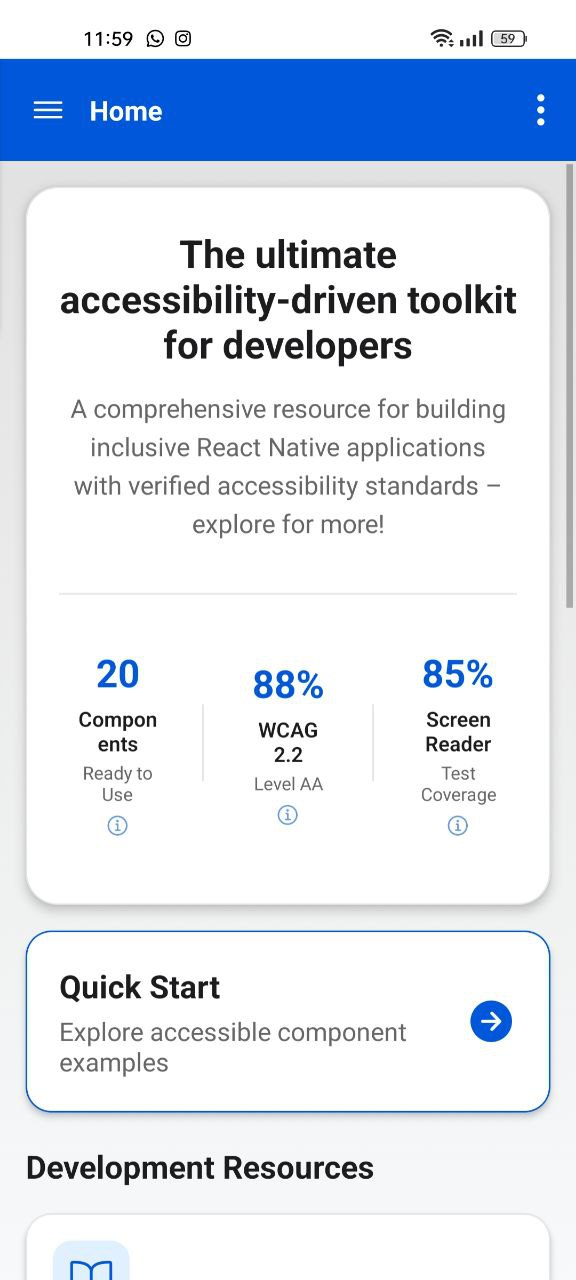
\includegraphics[width=0.4\linewidth, alt={Screenshot of the Home Screen of AccessibleHub}]{img/homescreen.jpg}
    \caption{The Home Screen of \textit{AccessibleHub}}\label{fig:homescreen}
    \end{figure}

\pagebreak

    \item \textbf{Accessible Components} - Developers can learn how to implement accessible UI components in their mobile applications (\ref{fig:components}). This section is divided into four subscreens, each focusing on a specific category of components:

    \begin{itemize}
        \item \textit{Buttons and Touchables}: It covers the implementation of accessible buttons and touchable elements. It provides code examples and best practices for ensuring that these interactive elements are perceivable, operable, and understandable by all users, including those with disabilities;

        \item \textit{Forms}: The subscreen focuses on creating accessible input forms, including text fields, checkboxes, radio buttons, and date/time pickers. It demonstrates how to properly label form elements, provide instructions and feedback, and ensure that forms can be navigated and completed using various input methods, such as keyboards and screen readers;

        \item \textit{Media}: In the Media subscreen, developers learn how to make media content, such as images, videos, and audio, accessible to users with visual or auditory impairments. This includes providing alternative text for images, captions for videos, and transcripts for audio content;

        \item \textit{Dialogs}: It covers the creation of accessible modal dialogs, popups, and alerts. It provides guidance on how to ensure that these elements are properly announced by screen readers, can be easily dismissed, and do not interfere with the user's ability to navigate the application, maintaining focus management and ensuring clear exit strategies;

       \item \textit{Advanced}: This particular subscreen covers elements like alerts, sliders, progress bars and tab navigation, analyzing how accessibility may regard different animated or interactive components for more complex gesture interactions used everyday by users.
    \end{itemize}

Throughout the Components section, code implementations are shared as examples, which developers can easily copy to their clipboard and integrate into their own projects. This hands-on approach allows developers to quickly apply the accessibility principles they learn and see the results in action.

\begin{figure}[ht]
\centering
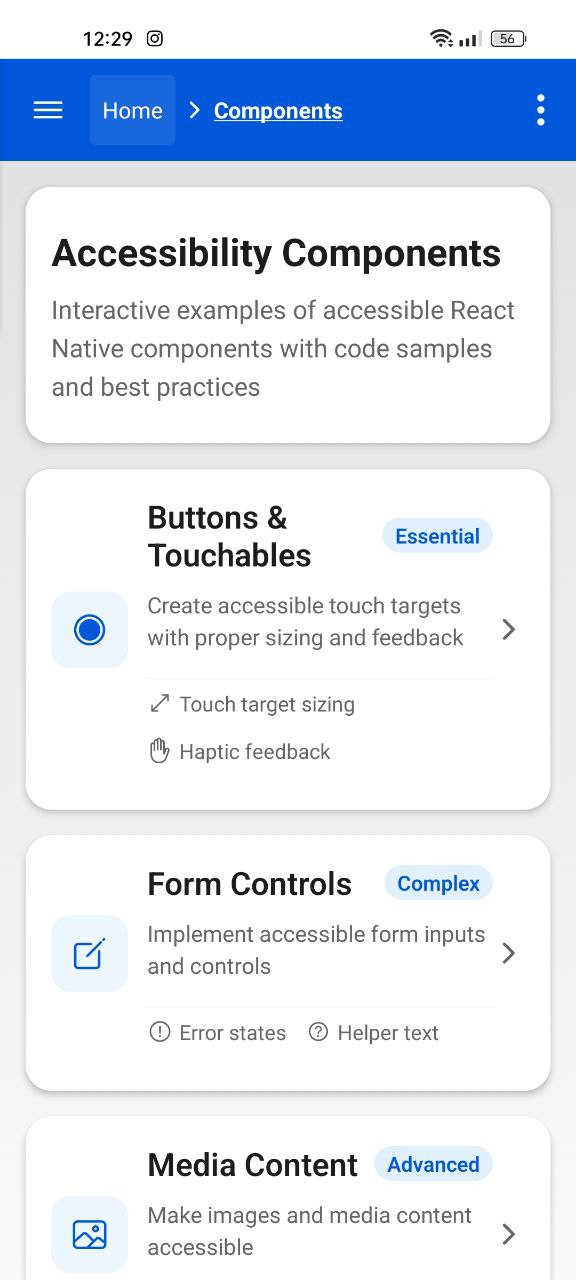
\includegraphics[width=0.4\linewidth, alt={Screenshot of the Components Screen of AccessibleHub}]{img/components.jpg}
\caption{The Components Screen of \textit{AccessibleHub}}\label{fig:components}
\end{figure}

\pagebreak

\item \textbf{Best Practices} - Designed to give developers a general understanding of the overarching principles and guidelines for creating accessible mobile applications (\ref{fig:best-practices}). It is divided into five subscreens, each addressing a key aspect of mobile accessibility:

    \begin{itemize}
        \item \textit{Gestures Tutorial}: This subscreen provides an overview of the various gesture interactions used in mobile applications and how to make them accessible to users with motor impairments or those relying on assistive technologies. It covers best practices for implementing alternative input methods and providing clear instructions and feedback. These gestures are general, tested to be used universally, both by everyday users and screen reader ones;

        \item \textit{Semantics Structure}: Here, developers learn about the importance of using semantic \textit{HTML} and \gls{ariag} roles to convey the structure and meaning of the application's content. This helps screen readers and other assistive technologies better understand and navigate the application;

        \item \textit{Navigation}: This one focuses on creating accessible navigation patterns, such as menus, tabs, and breadcrumbs. It provides guidance on how to ensure that navigation elements are properly labeled, can be operated using various input methods, and provide clear feedback to the user, jumping directly to the main context of a screen and bringing the attention to an element on-screen without distracting him from the action to be completed;

        \item \textit{Screen Reader Support}: This subscreen covers the specific considerations for making mobile applications compatible with screen readers, such as \gls{voiceover} on \textit{iOS} and \gls{talkback} on \textit{Android}. It includes best practices for labeling elements, providing alternative text, and ensuring that the application's content and functionality can be fully accessed and understood using a screen reader;

        \item \textit{Accessibility Guidelines}: The Accessibility Guidelines subscreen provides an overview of the key accessibility standards to be followed and a general list of principles to incorporate into a project, seeing how they apply to mobile application development. It helps developers understand the different levels of conformance and how to assess their application's accessibility against these guidelines.
    \end{itemize}

\begin{figure}[ht]
\centering
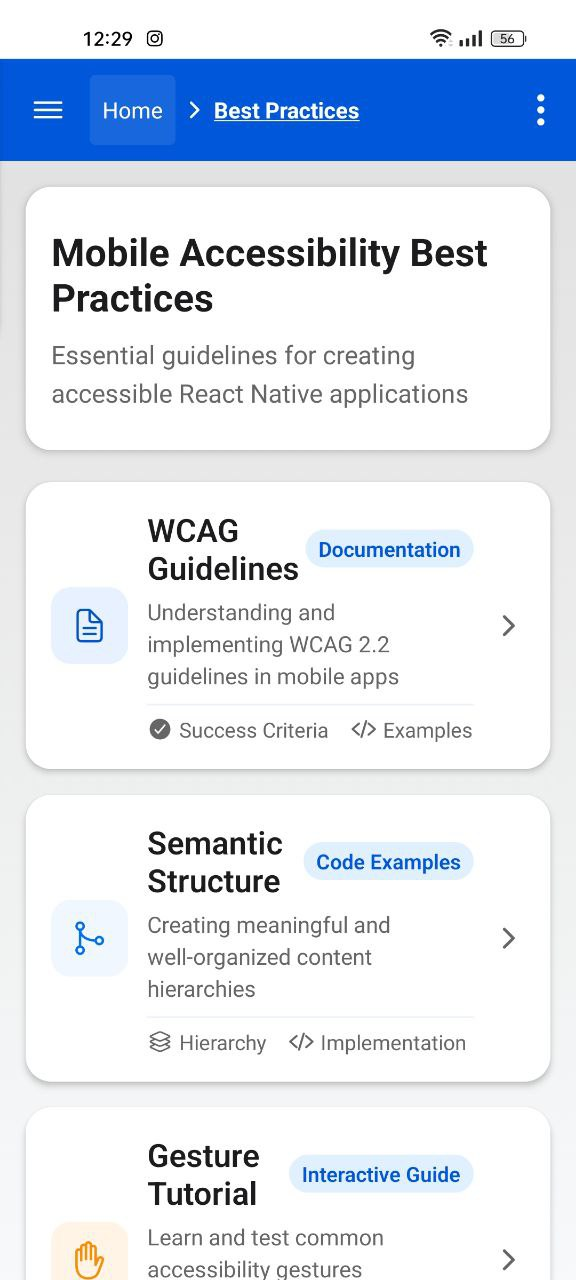
\includegraphics[width=0.4\linewidth, alt={Screenshot of the Best Practices Screen of AccessibleHub}]{img/best-practices.jpg}
\caption{The Best Practices Screen of \textit{AccessibleHub}}\label{fig:best-practices}
\end{figure}

\pagebreak

\item \textbf{Framework Comparison} - It provides a side-by-side comparison of the accessibility features and implementation differences between popular mobile development frameworks, such as React Native and Flutter (\ref{fig:frameworks-comparison}). This section helps developers understand how accessibility is handled in each framework and provides guidance on leveraging the specific accessibility APIs and tools available in each one. This is divided into different categories, offering a practical and formal overview on how such frameworks are compared with each other. By highlighting the similarities and differences between frameworks, developers can make informed decisions about which framework to use for their accessibility needs and how to optimize their implementations for each platform;

\begin{figure}[ht]
\centering
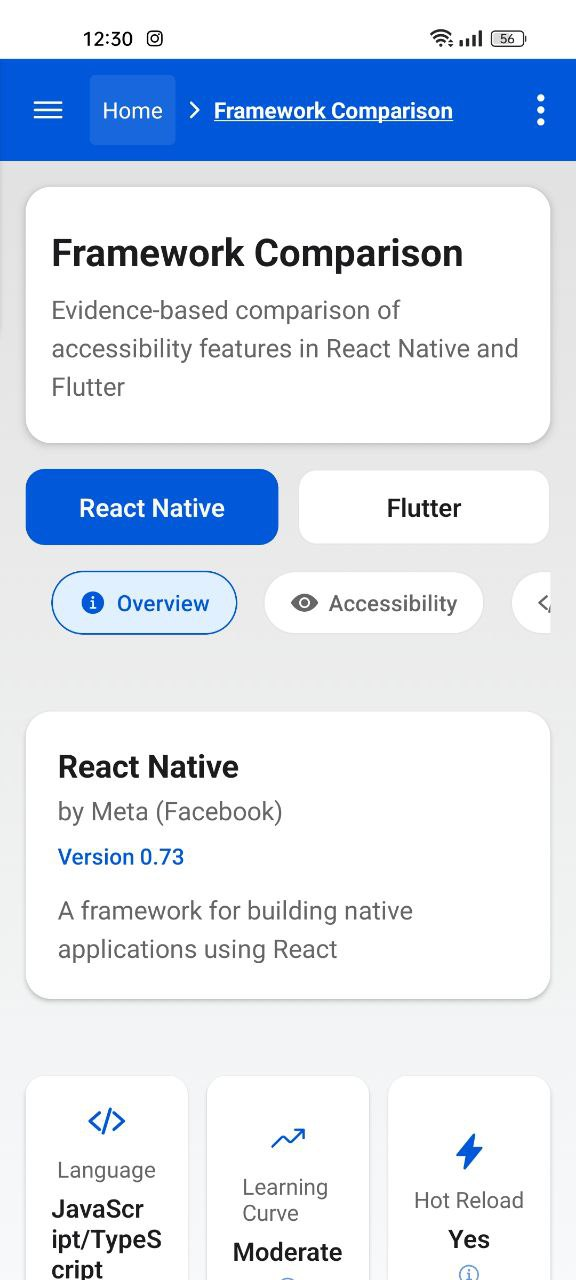
\includegraphics[width=0.4\linewidth, alt={Screenshot of the Frameworks Comparison Screen of AccessibleHub}]{img/frameworks-comparison.jpg}
\caption{The Frameworks Comparison Screen of \textit{AccessibleHub}}\label{fig:frameworks-comparison}
\end{figure}

\pagebreak

\item \textbf{Tools} - It serves as a central hub for accessing various accessibility-related tools and resources (\ref{fig:tools}). This includes links to official documentation, such as the React Native Accessibility \acrshort{api} reference and the \textit{Flutter Accessibility package} documentation. It also provides quick access to popular accessibility testing tools, such as \textit{Accessibility Scanner} for \textit{Android} and \textit{Accessibility Inspector} for \textit{iOS}. By consolidating these resources in one place, the Tools screen makes it easy for developers to find the information and tools they need to ensure their applications are fully accessible; 

\begin{figure}[ht]
\centering
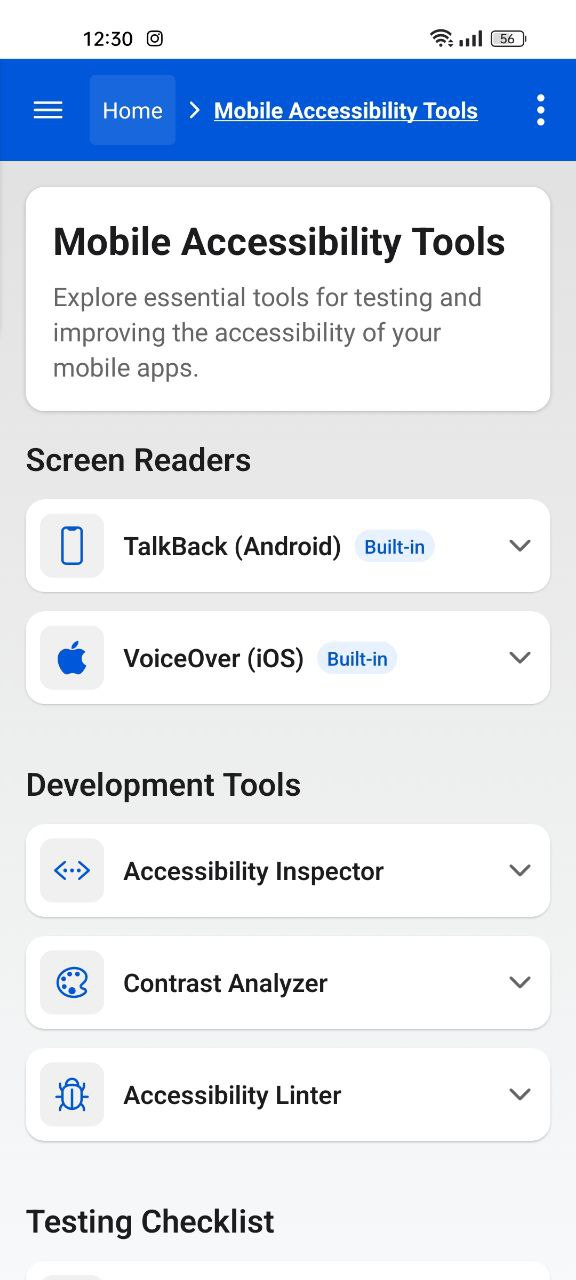
\includegraphics[width=0.4\linewidth, alt={Screenshot of the Tools Screen of AccessibleHub}]{img/tools.jpg}
\caption{The Tools Screen of \textit{AccessibleHub}}\label{fig:tools}
\end{figure}

\pagebreak

\item \textbf{Settings} - Allows users to customize various aspects of the \textit{AccessibleHub} application to suit their individual learning needs and preferences (\ref{fig:settings}). This includes options for adjusting the font size, color contrast (including options for gray scale and dark mode), reduced motion settings and others to help users and ensure the application itself is accessible to a wide range of users. It also provides information on how to configure the accessibility settings on the user's device, such as enabling screen readers or adjusting the display settings. By offering these customization options and guidance, the page reinforces the importance of accessibility as an everyday tool, meant to accompany practical user needs in an easy and quick way;

\begin{figure}[ht]
\centering
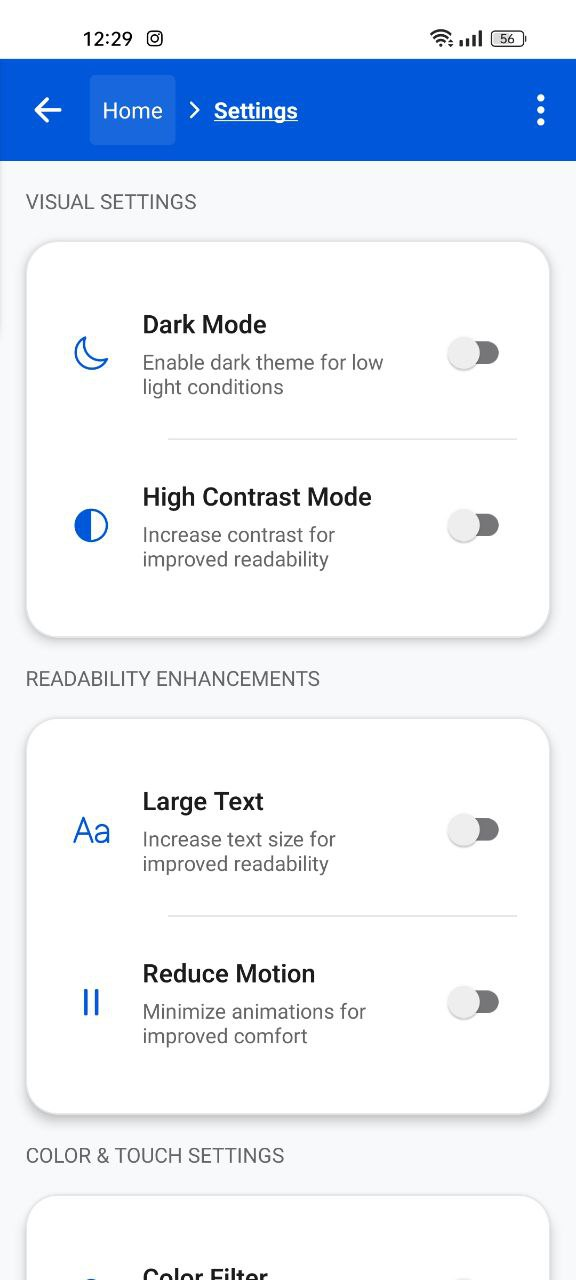
\includegraphics[width=0.4\linewidth, alt={Screenshot of the Settings Screen of AccessibleHub}]{img/settings.jpg}
\caption{The Settings Screen of \textit{AccessibleHub}}\label{fig:settings}
\end{figure}

\pagebreak

\item \textbf{Instruction and Community} - It provides a collaborative learning environment that extends beyond technical implementation (\ref{fig:instruction-community}). This section offers developers an opportunity to dive deeper into accessibility knowledge through curated resources and community engagement allowing for easier exploration towards other online resources. This provides an overview of currently open projects in the field of accessibility, provides advices on specific plugins and offers community examples of interest for a developers to be motivated into the creation of other accessible projects. By providing a platform for continuous learning and collaboration, this screen reinforces the importance of accessibility as a collective effort and a fundamental aspect of modern mobile application development.

\begin{figure}[ht]
\centering
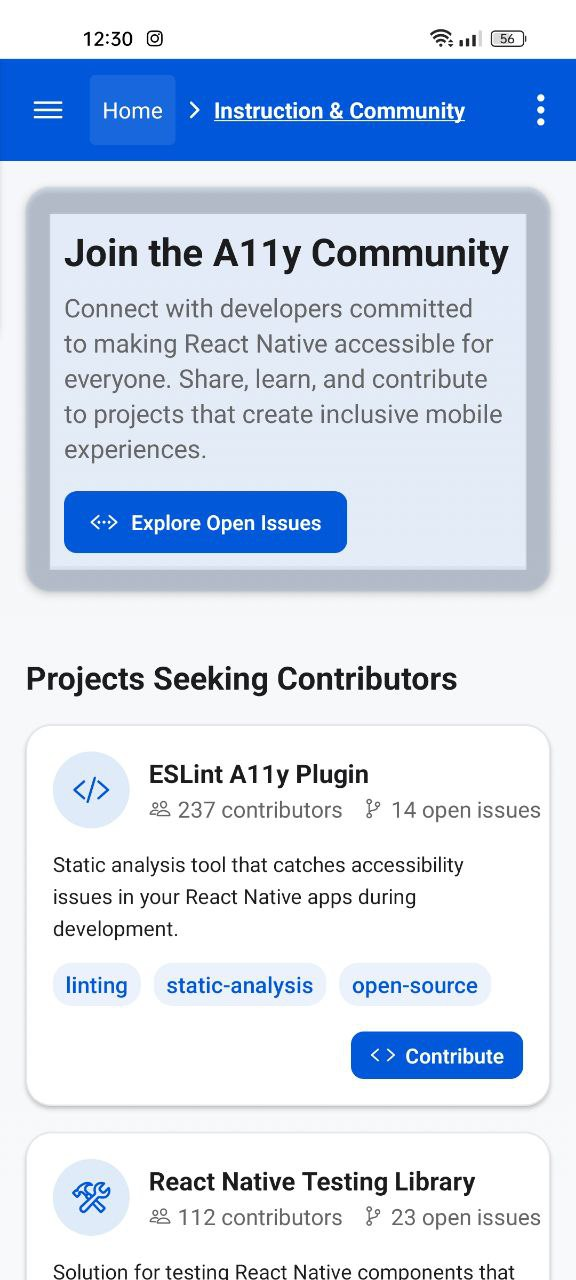
\includegraphics[width=0.4\linewidth, alt={Screenshot of the Instruction and Community Screen of AccessibleHub}]{img/instruction-community.jpg}
\caption{The Instruction and Community Screen of \textit{AccessibleHub}}\label{fig:instruction-community}
\end{figure}
    
\end{enumerate}

\pagebreak

\subsection{From guidelines to implementation: a screen-based methodology}

Accessibility guidelines and standards - most notably the \acrshort{wcagacr}  and related mobile-specific considerations—establish the formal foundation for inclusive digital design, as discussed in \ref{sec:accessibility-guidelines}. These criteria are essential but inherently abstract and can be challenging to implement directly in code. Building on Perinello and Gaggi's approach focusing solely on post-implementation testing, the methodology presented embeds accessibility into the development process. We do this by analyzing each screen of the application through a structured framework that connects theoretical requirements with practical implementation strategies. The approach to be considered is built following these layers:

\begin{enumerate}
    \item \textit{Theoretical foundation} – This layer encompasses the abstract principles and success criteria defined by \textit{WCAG}/\acrshort{mcagacr}. For example, \textit{WCAG}’s four core principles require that content be presented in ways users can perceive, interact with, and understand. These criteria serve as the benchmark for our analysis;

    \item \textit{Implementation pattern} – Here, we translate the abstract requirements into concrete code structures within a mobile development context. In \textit{AccessibleHub}, this involves the systematic use of React Native properties (such as \textit{accessibilityLabel}, \textit{accessibilityRole}, etc.) to ensure that \acrshort{ui} components satisfy the established guidelines;

    \item \textit{User interaction flow} – Finally, we consider how end users interact with these components. This includes the behavior of assistive technologies (like screen readers), proper focus management, and the overall usability of the component within its real-world context.
\end{enumerate}

To illustrate this methodology in practice, we first map the \textit{UI} elements of a representative screen to their corresponding semantic roles. Next, we link each component to the relevant \acrshort{wcagacr} and \acrshort{mcagacr} criteria presented in the previous subsections, noting both the minimum compliance requirements and potential enhancements. Finally, we describe the technical solution—specifically, how React Native accessibility code properties are applied to meet and exceed these standards. This structured approach not only bridges the gap between abstract guidelines and real-world coding tasks but also sets the stage for the more detailed, screen-by-screen analyses presented in the next section.

\section{Accessibility implementation guidelines}
\label{sec:implementation-guidelines}

Having established the overall architecture of \textit{AccessibleHub} and the guiding principles from both \textit{WCAG} and \textit{MCAG}, we now present a screen-by-screen analysis. Each subsection highlights the key \textit{success criteria} addressed, references relevant \textit{mobile-specific considerations}, and demonstrates practical solutions in React Native. Where applicable, we contrast these with Flutter's approach, building upon the insights from Gaggi and Perinello's approach \cite{budai2024mobile} analazying Budai's Flutter code - following guidelines and then giving advice into introducing new ones.

\subsection{Home screen}

The Home Screen serves as the primary entry point of the \textit{AccessibleHub} application. It provides key metrics on accessibility compliance (e.g., number of accessible components, \acrshort{wcagacr} conformance level) and direct navigation to core sections: \textit{Accessible Components} (Quick Start), \textit{Best Practices}, \textit{Testing Tools}, and the \textit{Framework Comparison}. An example of the interface is shown in Figure~\ref{fig:home_screens_sidebyside}.

\begin{figure}[ht]
    \centering
    \begin{subfigure}[b]{0.48\textwidth}
        \centering
        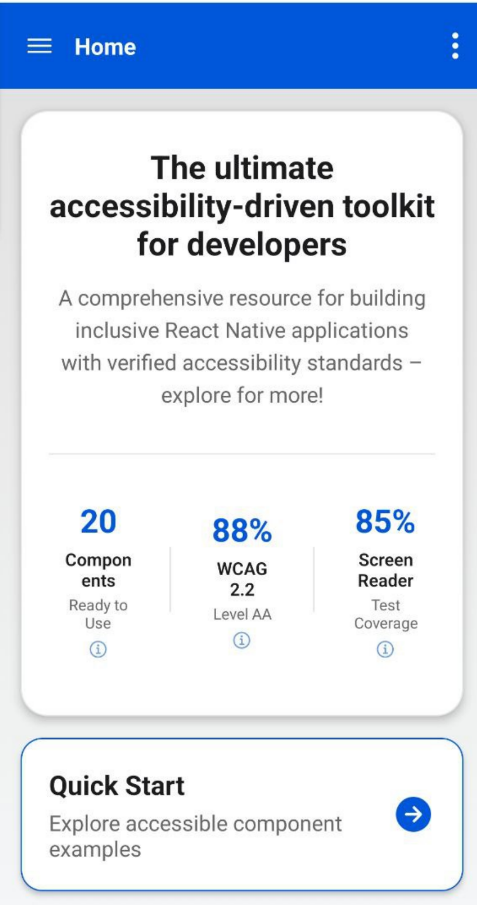
\includegraphics[width=\linewidth, alt={First part of the Home Screen}]{img/home1.png}
        \caption{Home screen - Part 1}
        \label{fig:home-left}
    \end{subfigure}
    \hfill
    \begin{subfigure}[b]{0.48\textwidth}
        \centering
        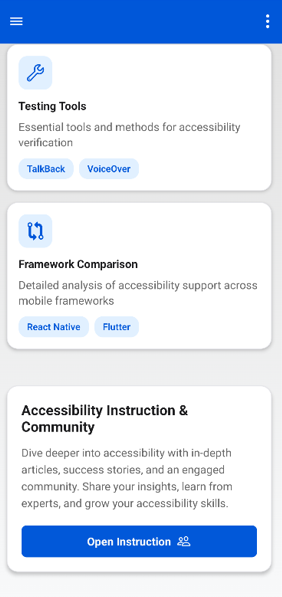
\includegraphics[width=\linewidth, alt={Second part of the Home Screen}]{img/home2.png}
        \caption{Home screen - Part 2}
        \label{fig:home-right}
    \end{subfigure}
    \caption{Side-by-side view of the two Home sections, with metrics and navigation buttons}
    \label{fig:home_screens_sidebyside}
\end{figure}

\subsubsection{Component inventory and WCAG/MCAG mapping}

Table~\ref{tab:component_criteria_mapping} provides a formal mapping between the UI components, their semantic roles, the specific WCAG 2.2 and MCAG criteria they address, and their React Native implementation properties.

\begin{longtable}{|p{2.5cm}|p{2cm}|p{2.8cm}|p{2.8cm}|p{4.3cm}|}
\caption{Home screen component-criteria mapping}
\label{tab:component_criteria_mapping}\\
\hline
\textbf{Component} & \textbf{Semantic Role} & \textbf{WCAG 2.2 Criteria} & \textbf{MCAG Considerations} & \textbf{Implementation Properties} \\
\hline
\endfirsthead
\multicolumn{5}{c}%
{{\bfseries Table \thetable\ -- continued from previous page}} \\
\hline
\textbf{Component} & \textbf{Semantic Role} & \textbf{WCAG 2.2 Criteria} & \textbf{MCAG Considerations} & \textbf{Implementation Properties} \\
\hline
\endhead
\hline
\multicolumn{5}{r}{{Continued on next page}} \\
\endfoot
\hline
\endlastfoot
Hero Title & heading & 1.4.3 Contrast (AA)\newline 2.4.6 Headings (AA) & Text readability on variable screen sizes & \texttt{accessibilityRole \ ="header"} \\
\hline
Stats Cards & button & 1.4.3 Contrast (AA)\newline 2.5.8 Target Size (AA)\newline 4.1.2 Name, Role, Value (A) & Touch target size\newline Non-essential information & \texttt{accessibilityRole \ ="button"}\newline \texttt{accessibilityLabel="\$\{value\}\% \$\{type\}, tap for details"}\newline \texttt{accessibilityHint="Shows \$\{type\} details"} \\
\hline
Decorative Icons & none & 1.1.1 Non-text Content (A) & Reduction of unnecessary focus stops & \texttt{accessibility \ ElementsHidden \ =true}\newline \texttt{important \ ForAccessibility="no"} \\
\hline
Quick Start Button & button & 1.4.3 Contrast (AA)\newline 2.5.8 Target Size (AA)\newline 2.5.2 Pointer Cancellation (A) & One-handed operation & \texttt{accessibilityRole \ ="button"}\newline \texttt{minHeight: 48}\newline \texttt{minWidth: 150} \\
\hline
Feature Cards & button & 1.3.1 Info and Relationships (A)\newline 1.4.3 Contrast (AA)\newline 2.5.8 Target Size (AA) & Logical grouping & \texttt{accessibilityRole \ ="button"}\newline \texttt{accessibilityLabel \ ="\$\{title\}"}\newline \texttt{accessibilityHint \ ="\$\{hint\}"} \\
\hline
Modal Dialog & dialog & 2.4.3 Focus Order (A)\newline 4.1.2 Name, Role, Value (A) & Keyboard trap prevention & \texttt{accessibilityRole \ ="dialog"}\newline Focus management implementation \\
\hline
Modal Tabs & tablist & 2.4.7 Focus Visible (AA)\newline 4.1.2 Name, Role, Value (A) & Touch interaction & \texttt{accessibilityRole \ ="tablist"}\newline \texttt{accessibility \ State= \ \{\{ selected: isActive \}\}} \\
\end{longtable}

\subsubsection{Formal metrics calculation methodology}

The Home Screen displays three key metrics that provide quantitative measurements of the application's accessibility. These metrics are not arbitrary but are calculated using a formal methodology defined in the \texttt{calculateAccessibilityScore} function within \texttt{index.tsx}. 

\begin{figure}[ht]
    \centering
    \begin{subfigure}[b]{0.48\textwidth}
        \centering
        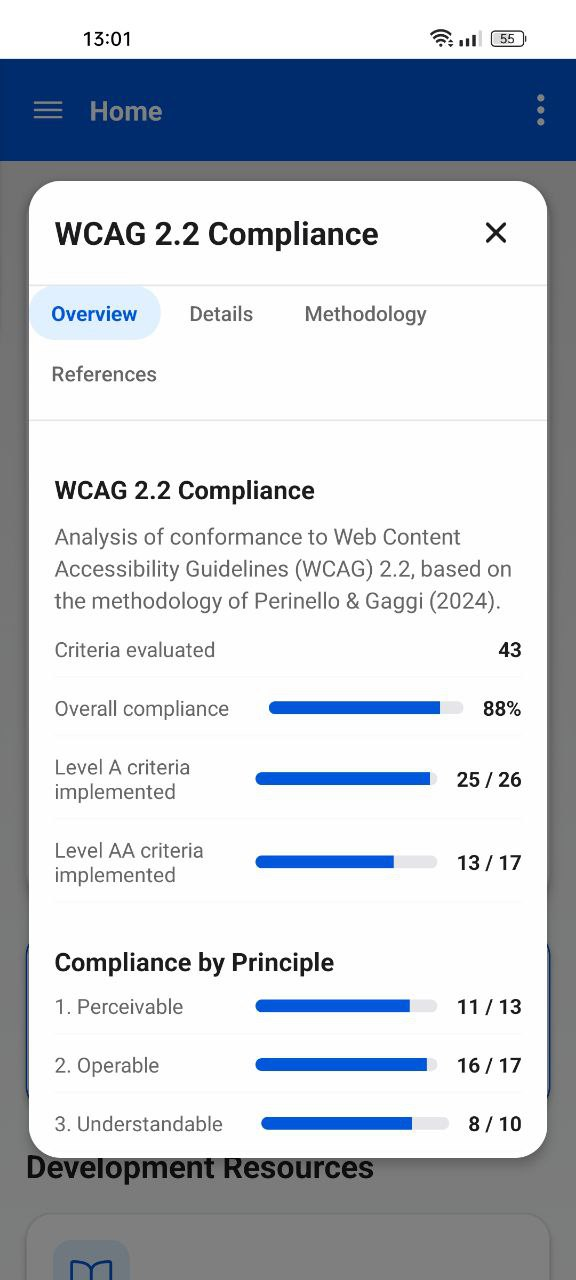
\includegraphics[width=\linewidth]{img/wcag-compliance.jpg}
        \caption{WCAG compliance overview}
        \label{fig:wcag-compliance-modal}
    \end{subfigure}
    \hfill
    \begin{subfigure}[b]{0.48\textwidth}
        \centering
        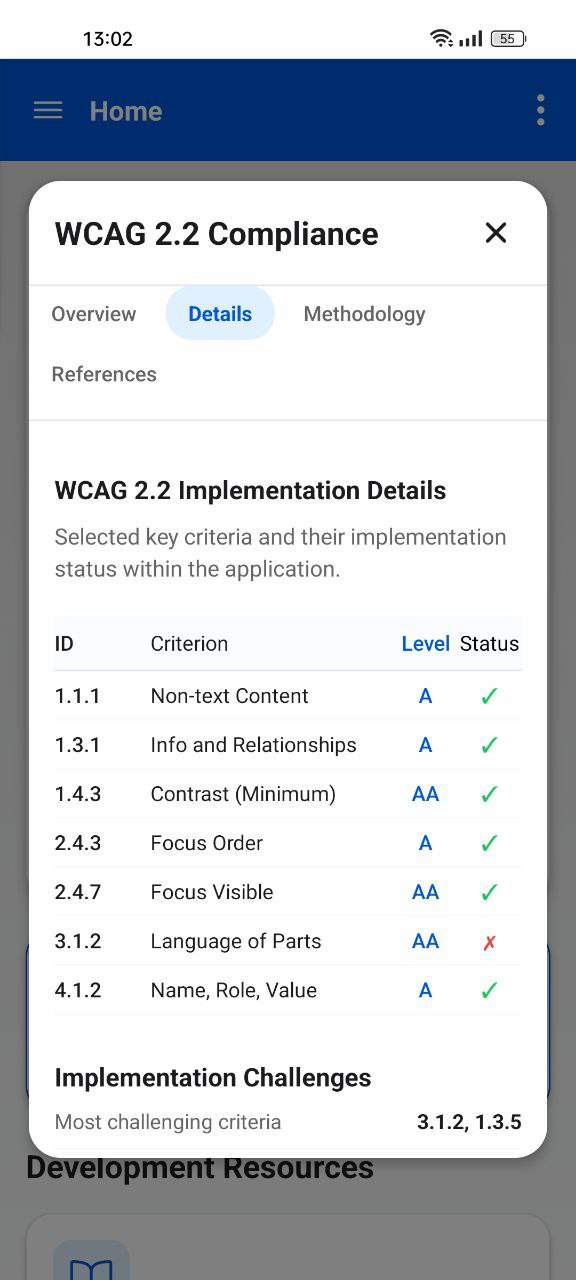
\includegraphics[width=\linewidth]{img/wcag-compliance-details.jpg}
        \caption{WCAG compliance details}
        \label{fig:wcag-details-modal}
    \end{subfigure}
    \caption{Modal dialogs showing WCAG compliance metrics}
    \label{fig:wcag_modal_pair}
\end{figure}

\begin{figure}[ht]
    \centering
    \begin{subfigure}[b]{0.48\textwidth}
        \centering
        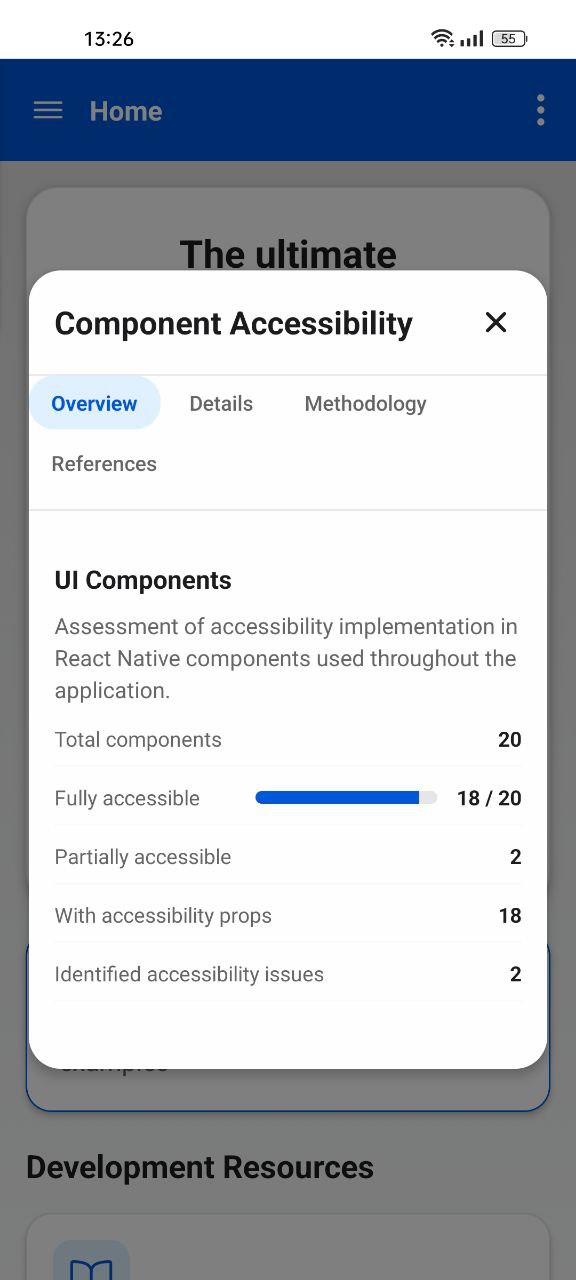
\includegraphics[width=\linewidth]{img/component-modal.jpg}
        \caption{Component metrics overview}
        \label{fig:component-overview-modal}
    \end{subfigure}
    \hfill
    \begin{subfigure}[b]{0.48\textwidth}
        \centering
        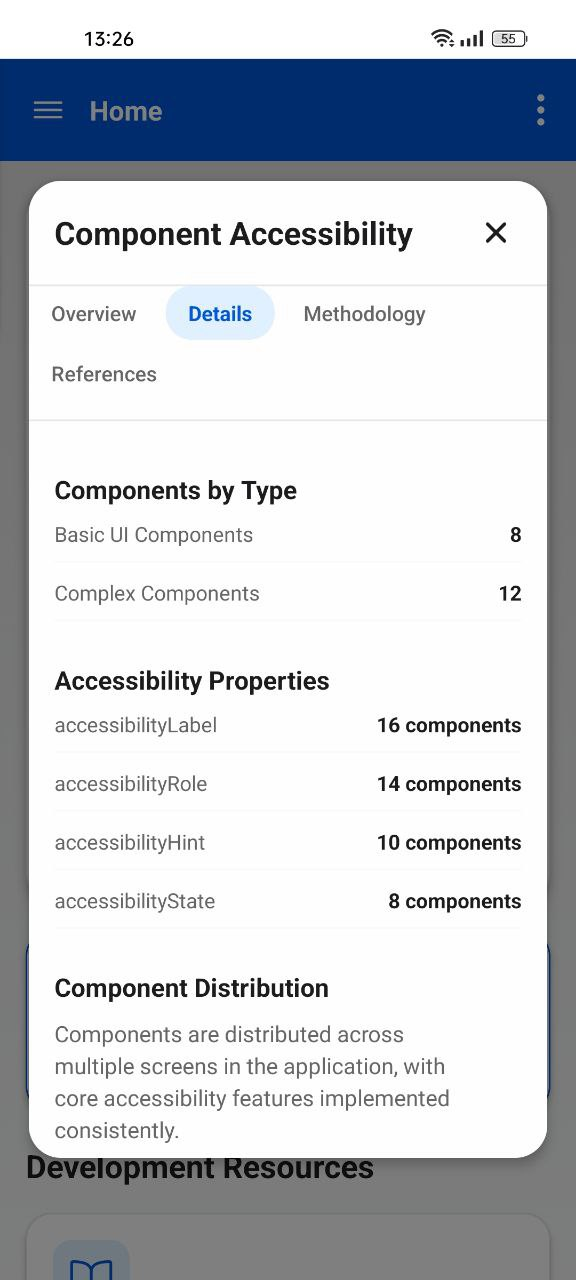
\includegraphics[width=\linewidth]{img/component-details.jpg}
        \caption{Component metrics details}
        \label{fig:component-details-modal}
    \end{subfigure}
    \caption{Modal dialogs showing component accessibility metrics}
    \label{fig:component_modal_pair}
\end{figure}

\begin{figure}[ht]
    \centering
    \begin{subfigure}[b]{0.48\textwidth}
        \centering
        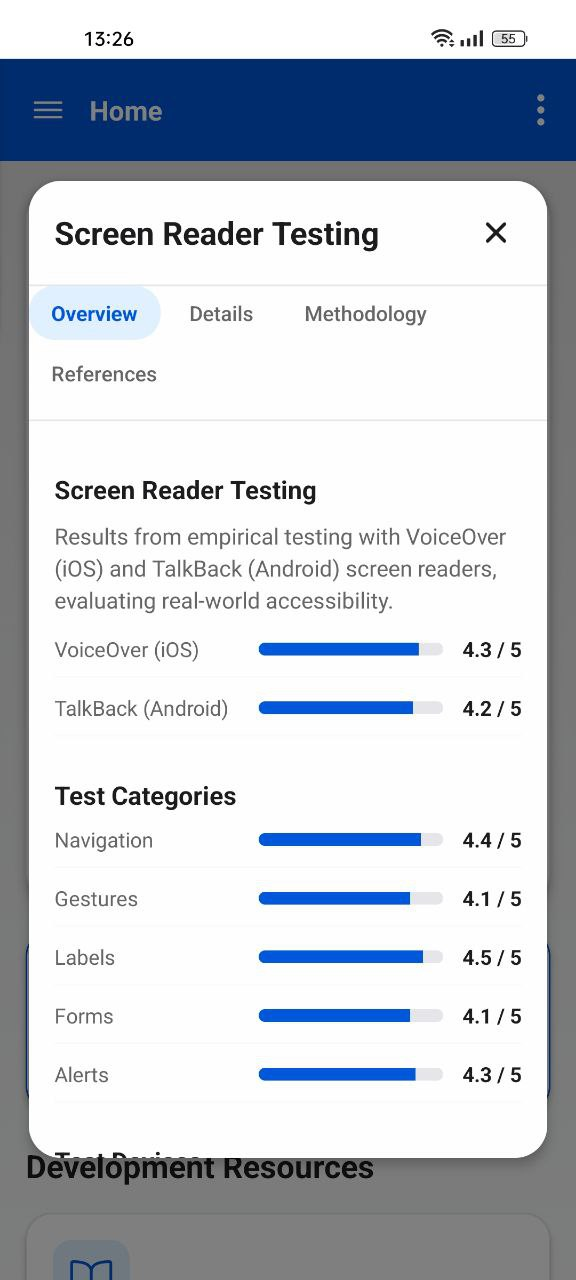
\includegraphics[width=\linewidth]{img/screen-reader-modal.jpg}
        \caption{Screen reader testing overview}
        \label{fig:screen-reader-overview}
    \end{subfigure}
    \hfill
    \begin{subfigure}[b]{0.48\textwidth}
        \centering
        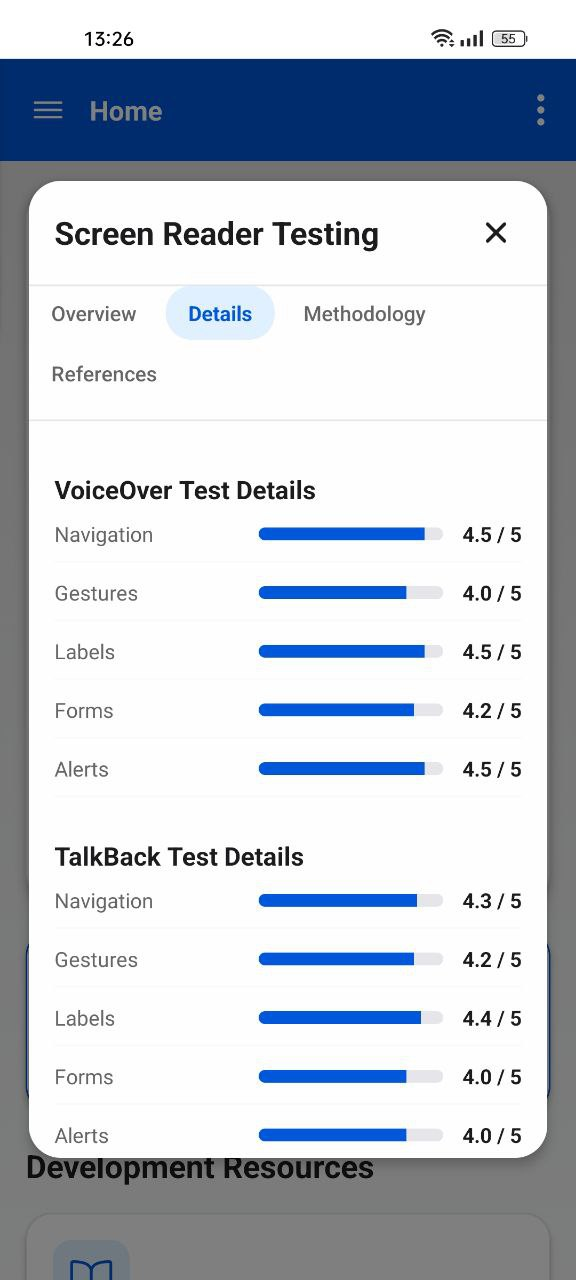
\includegraphics[width=\linewidth]{img/screen-reader-details.jpg}
        \caption{Screen reader testing details}
        \label{fig:screen-reader-details}
    \end{subfigure}
    \caption{Modal dialogs showing screen reader testing metrics}
    \label{fig:screen_reader_modals}
\end{figure}

\begin{figure}[ht]
    \centering
    \begin{subfigure}[b]{0.48\textwidth}
        \centering
        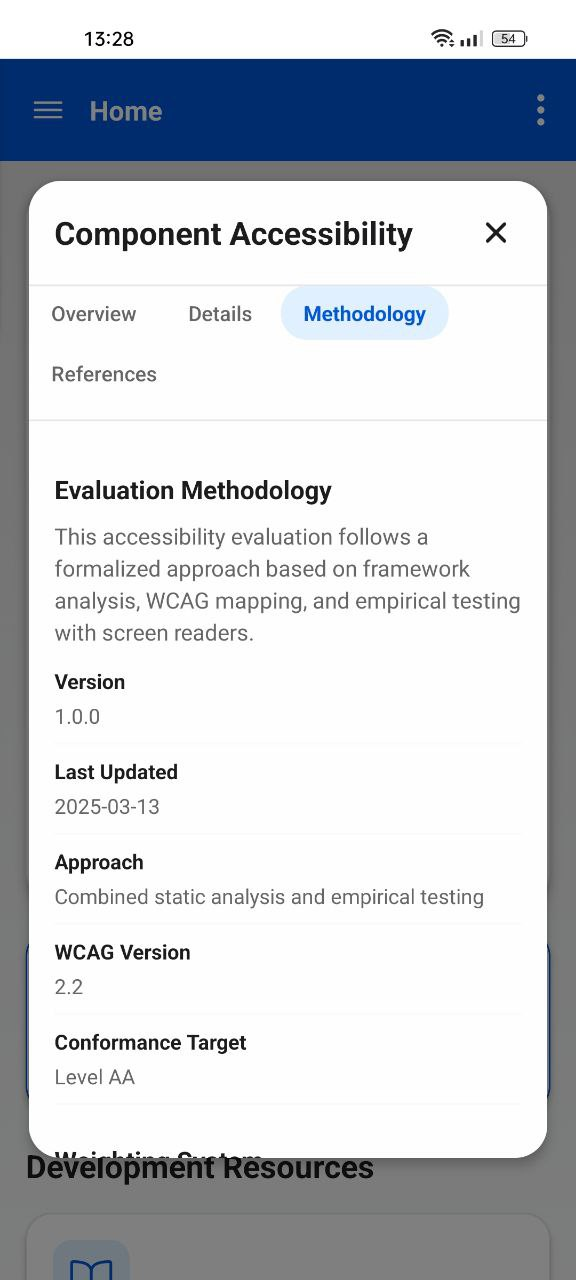
\includegraphics[width=\linewidth]{img/methodology.jpg}
        \caption{Methodology explanation}
        \label{fig:methodology-modal}
    \end{subfigure}
    \hfill
    \begin{subfigure}[b]{0.48\textwidth}
        \centering
        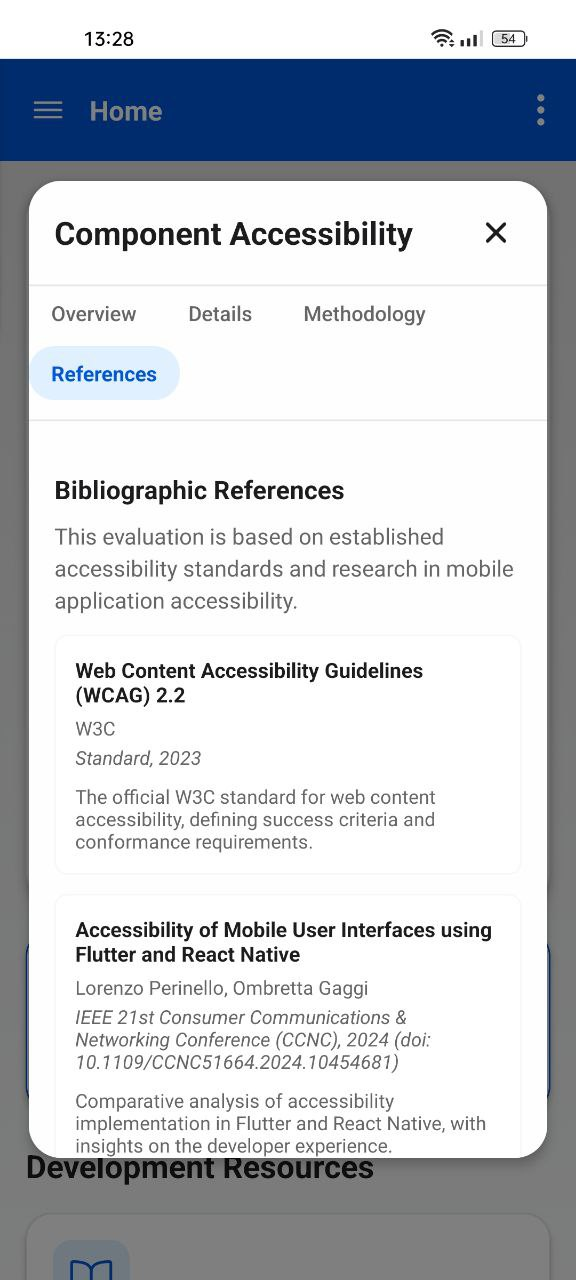
\includegraphics[width=\linewidth]{img/references.jpg}
        \caption{References documentation}
        \label{fig:references-modal}
    \end{subfigure}
    \caption{Modal dialogs showing methodology and references}
    \label{fig:methodology_references}
\end{figure}

\paragraph{Component accessibility score}

The Component Accessibility Score is calculated using the following formula:
\begin{equation}
\text{ComponentScore} 
= \left(\frac{\text{AccessibleComponents}}{\text{TotalComponents}}\right) \times 100
\end{equation}

Where:
\begin{itemize}
    \item \texttt{AccessibleComponents} = Number of components with properly implemented accessibility attributes (18)
    \item \texttt{TotalComponents} = Total number of UI components used in the application (20)
\end{itemize}

The implementation in \texttt{index.tsx} maintains a formal registry of all UI components, as shown by \ref{lst:component-registry}.

\begin{lstlisting}[
  style=ReactNativeStyle,
  caption={Component registry and calculation},
  label={lst:component-registry},
  basicstyle=\ttfamily\footnotesize,
  numbers=left,
]
// Component registry with accessibility status tracking
const componentsRegistry = {
  'button': { implemented: true, accessible: true, screens: ['home', 'gestures'] },
  'text': { implemented: true, accessible: true, screens: ['home', 'guidelines'] },
  // ... other components
  'tooltip': { implemented: true, accessible: false, screens: [] },
  // Total: 20 components, 18 fully accessible
};

// Component calculation
const componentsTotal = Object.keys(componentsRegistry).length;
const accessibleComponents = Object.values(componentsRegistry)
  .filter(c => c.implemented && c.accessible).length;
const componentScore = Math.round((accessibleComponents / componentsTotal) * 100);
\end{lstlisting}

\paragraph{WCAG compliance score}

The WCAG Compliance Score represents the percentage of implemented WCAG 2.2 success criteria across four principles:

\begin{equation}
\text{WCAGCompliance} 
= \left(\frac{\text{CriteriaLevelAMet} + \text{CriteriaLevelAAMet}}{\text{TotalCriteria}}\right) \times 100
\end{equation}

Where:
\begin{itemize}
    \item \texttt{CriteriaLevelAMet} = Number of Level A success criteria implemented (25)
    \item \texttt{CriteriaLevelAAMet} = Number of Level AA success criteria implemented (13)
    \item \texttt{TotalCriteria} = Total applicable WCAG criteria (43)
\end{itemize}

The implementation maintains a comprehensive tracking system for WCAG criteria, as shown by \ref{lst:wcag-tracking}.

\begin{lstlisting}[
  style=ReactNativeStyle,
  caption={WCAG criteria tracking and calculation},
  label={lst:wcag-tracking},
  basicstyle=\ttfamily\footnotesize,
  numbers=left,
]
// WCAG criteria tracking with implementation status
const wcagCriteria = {
  '1.1.1': { level: 'A', implemented: true, name: "Non-text Content" },
  '1.3.1': { level: 'A', implemented: true, name: "Info and Relationships" },
  // ... other criteria
  '4.1.3': { level: 'AA', implemented: true, name: "Status Messages" },
};

// WCAG compliance calculation
const criteriaValues = Object.values(wcagCriteria);
const totalCriteria = criteriaValues.length;
const levelACriteriaMet = criteriaValues
  .filter(c => c.level === 'A' && c.implemented).length;
const levelAACriteriaMet = criteriaValues
  .filter(c => c.level === 'AA' && c.implemented).length;
const wcagCompliance = Math.round(
  ((levelACriteriaMet + levelAACriteriaMet) / totalCriteria) * 100
);
\end{lstlisting}

\paragraph{Screen reader testing score}

The Screen Reader Testing Score represents empirical testing with VoiceOver (iOS) and TalkBack (Android):

\begin{equation}
\text{TestingScore} 
= \left(\frac{\text{VoiceOverAvg} + \text{TalkBackAvg}}{2}\right) \times 20
\end{equation}

Where:
\begin{itemize}
    \item \texttt{VoiceOverAvg} = Average score from VoiceOver testing across categories (4.34/5)
    \item \texttt{TalkBackAvg} = Average score from TalkBack testing across categories (4.18/5)
\end{itemize}

The scores are based on structured testing of five key aspects as shown by \ref{lst:screen-reader-testing}.

\begin{lstlisting}[
  style=ReactNativeStyle,
  caption={Screen reader testing results and calculation},
  label={lst:screen-reader-testing},
  basicstyle=\ttfamily\footnotesize,
  numbers=left,
]
// Screen reader test results from empirical testing
const screenReaderTests = {
  voiceOver: { // iOS
    navigation: 4.5, // Logical navigation flow
    gestures: 4.0,   // Gesture recognition
    labels: 4.5,     // Label clarity and completeness
    forms: 4.2,      // Form control accessibility
    alerts: 4.5      // Alert and dialog accessibility
  },
  talkBack: { // Android
    navigation: 4.3,
    gestures: 4.2,
    labels: 4.4,
    forms: 4.0,
    alerts: 4.0
  }
};

// Testing score calculation
const voiceOverScores = Object.values(screenReaderTests.voiceOver);
const talkBackScores = Object.values(screenReaderTests.talkBack);
const voiceOverAvg = voiceOverScores.reduce((sum, score) => 
  sum + score, 0) / voiceOverScores.length;
const talkBackAvg = talkBackScores.reduce((sum, score) => 
  sum + score, 0) / talkBackScores.length;
const testingScore = Math.round(((voiceOverAvg + talkBackAvg) / 2) * 20);
\end{lstlisting}

\paragraph{Overall accessibility score}

The overall accessibility score is calculated using weighted components:
\begin{equation}
\text{OverallScore} 
= (\text{ComponentScore} \times 0.4) 
+ (\text{WCAGCompliance} \times 0.4) 
+ (\text{TestingScore} \times 0.2)
\end{equation}

This weighting system gives equal importance to component implementation and standards compliance (40\% each), with empirical testing contributing 20\% to the final score.

\subsubsection{Technical implementation analysis}

The code sample present in \ref{lst:home-screen-accessibility} the key accessibility properties implemented in the Home Screen.

\begin{lstlisting}[
  style=ReactNativeStyle,
  caption={Annotated code sample demonstrating Home Screen accessibility properties},
  label={lst:home-screen-accessibility},
  basicstyle=\ttfamily\footnotesize,
  numbers=left,
]
// 1. ScrollView container with proper role and label
<ScrollView
  accessibilityRole="scrollview"
  accessibilityLabel="AccessibleHub Home Screen"
>
  {/* 2. Hero section with semantic heading */}
  <View style={themedStyles.heroCard}>
    <Text style={themedStyles.heroTitle} accessibilityRole="header">
      The ultimate accessibility-driven toolkit for developers
    </Text>

    {/* 3. Stats section with interactive metrics */}
    <View style={themedStyles.statsContainer}>
      <View style={themedStyles.statCard}>
        <TouchableOpacity
          style={themedStyles.touchableStat}
          onPress={() => openMetricDetails('component')}
          accessible
          accessibilityRole="button"
        >
          {/* 4. Content with accessibilityElementsHidden to prevent redundant 
              announcements */}
          <Text style={themedStyles.statNumber} accessibilityElementsHidden>
            {accessibilityMetrics.componentCount}
          </Text>
          <Text style={themedStyles.statLabel} accessibilityElementsHidden>
            Components
          </Text>
        </TouchableOpacity>
      </View>
  </View>

  {/* 6. Quick Start button with appropriate sizing for touch targets */}
  <TouchableOpacity
    style={themedStyles.quickStartCard}
    onPress={() => router.push('/components')}
    accessibilityRole="button"
    accessibilityLabel="Quick start with component examples"
    accessibilityHint="Navigate to components section"
  >
    <View style={themedStyles.cardText}>
      <Text style={themedStyles.cardTitle}>Quick Start</Text>
      <Text style={themedStyles.cardDescription}>
        Explore accessible component examples
      </Text>
    </View>
  </TouchableOpacity>
</ScrollView>
\end{lstlisting}

\subsubsection{Contrast and color analysis}

Table~\ref{tab:contrast_analysis} presents the formal contrast analysis for UI elements on the Home Screen. All elements meet at least WCAG Level~AA requirements (4.5:1 for normal text).

\begin{longtable}{|p{2.8cm}|p{2.8cm}|p{2.8cm}|p{2.4cm}|p{2.4cm}|}
\caption{Home screen contrast analysis}
\label{tab:contrast_analysis}\\
\hline
\textbf{UI Element} & \textbf{Foreground Color} & \textbf{Background Color} & \textbf{Contrast Ratio} & \textbf{WCAG Compliance} \\
\hline
\endfirsthead
\multicolumn{5}{c}%
{{\bfseries Table \thetable\ -- continued from previous page}} \\
\hline
\textbf{UI Element} & \textbf{Foreground Color} & \textbf{Background Color} & \textbf{Contrast Ratio} & \textbf{WCAG Compliance} \\
\hline
\endhead
\hline
\multicolumn{5}{r}{{Continued on next page}} \\
\endfoot
\hline
\endlastfoot
Hero Title & \#000000 (Light)\newline \#FFFFFF (Dark) & \#FFFFFF (Light)\newline \#121212 (Dark) & 21:1 (Light)\newline 21:1 (Dark) & AAA ($\ge7{:}1$) \\
\hline
Subtitle & \#6B7280 (Light)\newline \#A0AEC0 (Dark) & \#FFFFFF (Light)\newline \#121212 (Dark) & 4.6:1 (Light)\newline 5.2:1 (Dark) & AA ($\ge4.5{:}1$) \\
\hline
Stat Numbers & \#0066CC (Light)\newline \#3B82F6 (Dark) & \#FFFFFF (Light)\newline \#121212 (Dark) & 4.7:1 (Light)\newline 5.1:1 (Dark) & AA ($\ge4.5{:}1$) \\
\hline
Quick Start Button & \#FFFFFF & \#0066CC & 4.8:1 & AA ($\ge4.5{:}1$) \\
\hline
Feature Card Titles & \#000000 (Light)\newline \#FFFFFF (Dark) & \#FFFFFF (Light)\newline \#1E293B (Dark) & 21:1 (Light)\newline 16:1 (Dark) & AAA ($\ge7{:}1$) \\
\end{longtable}

\subsubsection{Screen reader support analysis}

Table~\ref{tab:screen_reader_analysis} presents results from systematic testing of the Home Screen with screen readers on both iOS and Android platforms.

\begin{longtable}{|p{2.8cm}|p{3.5cm}|p{3.5cm}|p{4cm}|}
\caption{Home screen screen reader testing results}
\label{tab:screen_reader_analysis}\\
\hline
\textbf{Test Case} & \textbf{VoiceOver (iOS 16)} & \textbf{TalkBack (Android 14-15)} & \textbf{WCAG Criteria Addressed} \\
\hline
\endfirsthead
\multicolumn{4}{c}%
{{\bfseries Table \thetable\ -- continued from previous page}} \\
\hline
\textbf{Test Case} & \textbf{VoiceOver (iOS 16)} & \textbf{TalkBack (Android 14-15)} & \textbf{WCAG Criteria Addressed} \\
\hline
\endhead
\hline
\multicolumn{4}{r}{{Continued on next page}} \\
\endfoot
\hline
\endlastfoot
Hero Title & \ding{51} Announces ``The ultimate accessibility-driven toolkit for developers, heading'' & \ding{51} Announces ``The ultimate accessibility-driven toolkit for developers, heading'' & 1.3.1 - Info and Relationships (Level A), 2.4.6 - Headings and Labels (Level AA) \\
\hline
Metrics Cards & \ding{51} Announces full label with metrics and hint & \ding{51} Announces full label with metrics and hint & 1.3.1 Info and Relationships (Level A), 4.1.2 Name, Role, Value (Level A) \\
\hline
Quick Start Button & \ding{51} Announces ``Quick start with component examples, button'' & \ding{51} Announces ``Quick start with component examples, button'' & 2.4.4 Link Purpose (In Context) (Level A), 4.1.2 Name, Role, Value (Level A) \\
\hline
Feature Cards & \ding{51} Announces title and hint & \ding{51} Announces title and hint & 2.4.4 Link Purpose (In Context) (Level A), 4.1.2 Name, Role, Value (Level A) \\
\hline
Modal Dialog Opening & \ding{51} Focus moves to dialog title & \ding{51} Focus moves to dialog title & 2.4.3 Focus Order (Level A) \\
\hline
Modal Tab Navigation & \ding{51} Announces tab selection state & \ding{51} Announces tab selection state & 4.1.2 Name, Role, Value (Level A) \\
\hline
Modal Dialog Closing & \ding{51} Focus returns to triggering element & \ding{54} Occasional focus loss (fixed in v1.0.3) & 2.4.3 Focus Order (Level A) \\
\end{longtable}

The implementation addresses several key MCAG considerations:
\begin{enumerate}
    \item \textbf{Swipe optimization}: Decorative elements are marked with \\ \texttt{importantForAccessibility="no"} to reduce unnecessary swipes;
    \item \textbf{Clear instructions}: The modal tabs implementation provides clear state announcements, ensuring screen reader users understand the current selection;
    \item \textbf{Platform-specific adaptations}: The implementation accounts for differences between VoiceOver and TalkBack behavior, as evidenced by the test results.
\end{enumerate}

\subsubsection{Implementation overhead analysis}

Table~\ref{tab:implementation_overhead} quantifies the additional code required to implement accessibility features in the Home Screen.

\begin{longtable}{|p{3.8cm}|p{2.3cm}|p{2.8cm}|p{2.8cm}|}
\caption{Accessibility implementation overhead}
\label{tab:implementation_overhead}\\
\hline
\textbf{Accessibility Feature} & \textbf{Lines of Code} & \textbf{Percentage of Total} & \textbf{Complexity Impact} \\
\hline
\endfirsthead
\multicolumn{4}{c}%
{{\bfseries Table \thetable\ -- continued from previous page}} \\
\hline
\textbf{Accessibility Feature} & \textbf{Lines of Code} & \textbf{Percentage of Total} & \textbf{Complexity Impact} \\
\hline
\endhead
\hline
\multicolumn{4}{r}{{Continued on next page}} \\
\endfoot
\hline
\endlastfoot
Semantic Roles & 12 LOC & 2.1\% & Low \\
\hline
Descriptive Labels & 24 LOC & 4.3\% & Medium \\
\hline
Element Hiding & 8 LOC & 1.4\% & Low \\
\hline
Focus Management & 18 LOC & 3.2\% & Medium \\
\hline
Contrast Handling & 16 LOC & 2.9\% & Medium \\
\hline
Metrics Calculation & 78 LOC & 14.1\% & High \\
\hline
\textbf{Total} & \textbf{156 LOC} & \textbf{28.0\%} & \textbf{Medium-High} \\
\end{longtable}

This analysis reveals that implementing comprehensive accessibility adds approximately 28\% to the code base of the Home Screen, with the metrics calculation system representing the most significant component. This overhead is justified by the improved user experience for people with disabilities and the educational value for developers learning to implement accessibility.

\subsubsection{WCAG conformance by principle}

Table~\ref{tab:wcag_by_principle} provides a detailed analysis of WCAG 2.2 compliance by principle:

\begin{longtable}{|p{2.5cm}|p{3.8cm}|p{3.2cm}|p{5.2cm}|}
\caption{WCAG compliance analysis by principle}
\label{tab:wcag_by_principle}\\
\hline
\textbf{Principle} & \textbf{Description} & \textbf{Implementation Level} & \textbf{Key Success Criteria} \\
\hline
\endfirsthead
\multicolumn{4}{c}%
{{\bfseries Table \thetable\ -- continued from previous page}} \\
\hline
\textbf{Principle} & \textbf{Description} & \textbf{Implementation Level} & \textbf{Key Success Criteria} \\
\hline
\endhead
\hline
\multicolumn{4}{r}{{Continued on next page}} \\
\endfoot
\hline
\endlastfoot
1. Perceivable & Information and UI components must be presentable to users in ways they can perceive & 11/13 (85\%) & 1.1.1 Non-text Content (A)\newline 1.3.1 Info and Relationships (A)\newline 1.4.3 Contrast (Minimum) (AA) \\
\hline
2. Operable & UI components and navigation must be operable & 16/17 (94\%) & 2.4.3 Focus Order (A)\newline 2.4.7 Focus Visible (AA)\newline 2.5.8 Target Size (Minimum) (AA) \\
\hline
3. Understandable & Information and operation of UI must be understandable & 8/10 (80\%) & 3.2.1 On Focus (A)\newline 3.2.4 Consistent Identification (AA)\newline 3.3.2 Labels or Instructions (A) \\
\hline
4. Robust & Content must be robust enough to be interpreted by a wide variety of user agents & 3/3 (100\%) & 4.1.1 Parsing (A)\newline 4.1.2 Name, Role, Value (A)\newline 4.1.3 Status Messages (AA) \\
\end{longtable}

\subsubsection{Mobile-specific considerations}

The Home Screen implementation addresses several mobile-specific accessibility considerations beyond standard WCAG requirements:

\begin{enumerate}
    \item \textbf{Touch target sizing}: All interactive elements maintain minimum dimensions of 48$\times$48dp, exceeding the WCAG 2.5.8 requirement of 24$\times$24px and addressing the mobile-specific need for larger touch targets;
    \item \textbf{Reduced motion support}: The implementation respects the device's reduced motion settings and provides an in-app toggle, addressing vestibular disorders that are particularly relevant in mobile contexts;
    \item \textbf{Dark mode support}: The application's theming system adapts to both light and dark modes, addressing the mobile-specific need for readability in various lighting conditions;
    \item \textbf{Screen reader gesture optimization}: The implementation carefully manages focus to ensure efficient navigation with touch gestures, as shown in the screen reader testing results;
    \item \textbf{One-handed operation}: The layout places primary interactive elements within reach of a thumb during one-handed use, a critical mobile accessibility consideration not explicitly covered by WCAG.
\end{enumerate}

\subsubsection{Beyond WCAG: metrics-driven accessibility guidelines}

The Home Screen implementation highlights several accessibility principles that extend beyond standard WCAG requirements, specifically addressing quantitative accessibility evaluation in mobile applications:

\begin{enumerate}
    \item \textbf{Comprehensive metrics visualization}: Accessibility compliance should be quantified and presented in a transparent, understandable format. The Home Screen implements this through dedicated metric cards with clear visual indicators of implementation status, moving beyond binary compliance to represent different degrees of accessibility achievement;
    
    \item \textbf{Multi-dimensional evaluation framework}: Accessibility assessment should consider multiple dimensions including component implementation (40\%), standards compliance (40\%), and empirical testing (20\%). This weighted approach, implemented in the metrics calculation system, recognizes that true accessibility extends beyond technical conformance to include real-world usability;
    
    \item \textbf{Transparency in methodology}: Applications should provide clear documentation of accessibility evaluation methodology including test devices, standards versions, and measurement approaches. The modal details system implements this principle by exposing the entire evaluation framework to users, creating accountability in accessibility claims;
    
    \item \textbf{Academic grounding principle}: Accessibility implementations benefit from explicit connection to peer-reviewed research and formal standards. The References tab implements this by connecting implementation practices to specific academic papers and standards documentation;
    
    \item \textbf{Progressive disclosure of complexity}: Technical accessibility details should be organized in layers of increasing complexity, allowing users to access the appropriate level of detail for their needs. The tabbed modal system implements this by separating overview information from detailed implementation specifics.
\end{enumerate}

These guidelines extend WCAG by formalizing the quantitative evaluation of accessibility status, providing developers with concrete metrics to track implementation progress rather than treating accessibility as a binary, achieved/not-achieved state.

\subsection{Accessible components main screen}

The Accessible Components Screen serves as a catalog of reusable accessibility patterns organized by component type. It provides developers with access to implementations of common UI elements with accessibility features properly integrated. Each component category includes implementation examples, best practices, and copy-ready code samples. The screen functions as an educational index, directing developers to detailed implementations of specific accessible components. Figure~\ref{fig:components_screens_sidebyside} shows the Components Screen interface.

\begin{figure}[ht]
    \centering
    \begin{subfigure}[b]{0.48\textwidth}
        \centering
        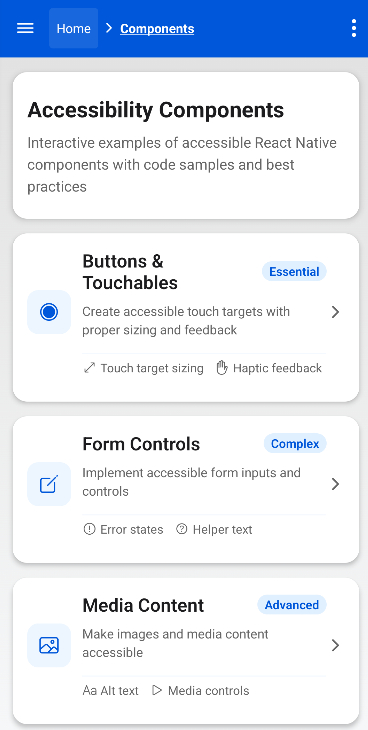
\includegraphics[width=\linewidth, alt={First part of the Components Screen}]{img/components1.png}
        \caption{Components screen - Top section}
        \label{fig:components-top}
    \end{subfigure}
    \hfill
    \begin{subfigure}[b]{0.48\textwidth}
        \centering
        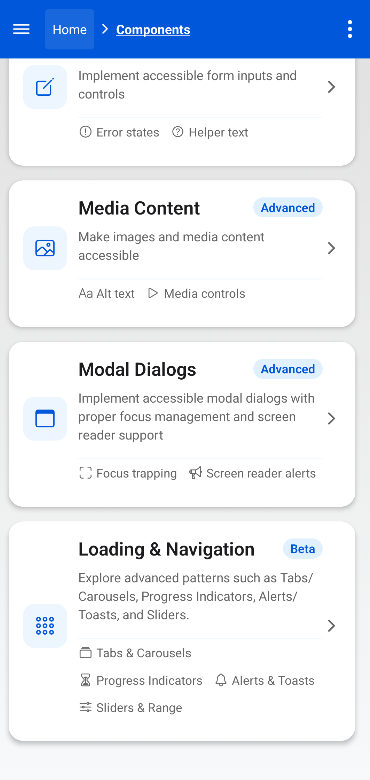
\includegraphics[width=\linewidth, alt={Second part of the Components Screen}]{img/components2.png}
        \caption{Components screen - Bottom section}
        \label{fig:components-bottom}
    \end{subfigure}
    \caption{Side-by-side view of the Components Screen sections, showing component categories}
    \label{fig:components_screens_sidebyside}
\end{figure}

\subsubsection{Component inventory and WCAG/MCAG mapping}

Table~\ref{tab:components_screen_mapping} provides a formal mapping between the UI components, their semantic roles, the specific WCAG 2.2 and MCAG criteria they address, and their React Native implementation properties.

\begin{longtable}{|p{2.5cm}|p{2cm}|p{2.8cm}|p{2.8cm}|p{4.3cm}|}
\caption{Components screen component-criteria mapping}
\label{tab:components_screen_mapping}\\
\hline
\textbf{Component} & \textbf{Semantic Role} & \textbf{WCAG 2.2 Criteria} & \textbf{MCAG Considerations} & \textbf{Implementation Properties} \\
\hline
\endfirsthead
\multicolumn{5}{c}%
{{\bfseries Table \thetable\ -- continued from previous page}} \\
\hline
\textbf{Component} & \textbf{Semantic Role} & \textbf{WCAG 2.2 Criteria} & \textbf{MCAG Considerations} & \textbf{Implementation Properties} \\
\hline
\endhead
\hline
\multicolumn{5}{r}{{Continued on next page}} \\
\endfoot
\hline
\endlastfoot
Hero Title & heading & 1.4.3 Contrast (AA)\newline 2.4.6 Headings (AA) & Text readability on variable screen sizes & \texttt{accessibilityRole \ ="header"} \\
\hline
Component Cards & button & 1.4.3 Contrast (AA)\newline 2.5.8 Target Size (AA)\newline 4.1.2 Name, Role, Value (A)\newline 2.4.4 Link Purpose (A) & Touch target size\newline Meaningful labels\newline Single finger operation & \texttt{accessibilityRole \ ="button"}\newline \texttt{accessibilityLabel=}\newline \texttt{onPress=handle \ ComponentPress} \\
\hline
Badges (Essential, Complex, etc.) & text & 1.4.3 Contrast (AA)\newline 1.3.1 Info and Relationships (A) & Descriptive labeling\newline Non-interactive elements & Part of parent button's \texttt{accessibilityLabel} \\
\hline
Decorative Icons & none & 1.1.1 Non-text Content (A) & Reduction of unnecessary focus stops & \texttt{accessibilityElements \ Hidden=true} \\
\hline
Breadcrumb Navigation & navigation & 2.4.4 Link Purpose (A)\newline 2.4.8 Location (AAA)\newline 3.2.3 Consistent Navigation (AA) & Context retention\newline Current location & \texttt{accessibilityRole \ ="button"}\newline \texttt{accessibilityLabel \ ="Go to \$\{label\}"} \\
\hline
Drawer Menu & menu & 2.4.3 Focus Order (A)\newline 4.1.2 Name, Role, Value (A)\newline 3.2.3 Consistent Navigation (AA) & Keyboard trap prevention\newline Persistent navigation & \texttt{accessibilityRole \ ="menu"}\newline \texttt{accessibilityLabel \ ="Main navigation menu"} \\
\hline
Drawer Menu Items & menuitem & 2.4.7 Focus Visible (AA)\newline 4.1.2 Name, Role, Value (A) & Touch interaction\newline Current location & \texttt{accessibilityRole \ ="menuitem"}\newline \texttt{accessibility \ State= \ \{\{ selected: isActive \}\}} \\
\end{longtable}

\subsubsection{Navigation and orientation analysis}

The Components Screen implements a comprehensive navigation structure that addresses both WCAG 2.4 (Navigable) and MCAG considerations for mobile devices. This structure includes three key elements that work together to provide clear orientation for all users:

\paragraph{Breadcrumb implementation}

The application as shown in \ref{fig:drawer-navigation} includes a hierarchical breadcrumb system in the header. This addresses WCAG 2.4.8 Location (Level AAA) by providing explicit path information. The breadcrumb implementation:

\begin{enumerate}
    \item Displays the current location in the application hierarchy;
    \item Provides interactive elements to navigate to parent screens;
    \item Uses consistent visual styling to indicate the current position;
    \item Implements proper focus management between screens.
\end{enumerate}

The breadcrumb is implemented with proper semantic roles and accessibility labels to ensure screen reader compatibility, as per \ref{lst:breadcrumb-implementation}.

\begin{lstlisting}[
  style=ReactNativeStyle,
  caption={Breadcrumb implementation with accessibility properties},
  label={lst:breadcrumb-implementation},
  basicstyle=\ttfamily\footnotesize,
  numbers=left,
]
<View style={styles.breadcrumbContainer}>
  <TouchableOpacity
    onPress={() => router.replace(`/${mapping.parentRoute}`)}
    accessibilityRole="button"
    accessibilityLabel={`Go to ${mapping.parentLabel}`}
    style={{
      padding: 8,
      minWidth: 40,
      minHeight: 44,
      justifyContent: 'center',
      backgroundColor: 'rgba(255, 255, 255, 0.1)',
      borderRadius: 4
    }}
  >
    <Text style={[styles.breadcrumbText, { fontWeight: 'normal' }]}>
      {mapping.parentLabel}
    </Text>
  </TouchableOpacity>
  <Ionicons
    name="chevron-forward"
    size={16}
    color={HEADER_TEXT_COLOR}
    style={{ marginHorizontal: 4 }}
    importantForAccessibility="no"
    accessibilityElementsHidden
  />
  <Text
    style={[styles.breadcrumbText, { fontWeight: 'bold', textDecorationLine: 'underline'}]}
    accessibilityLabel={`Current screen: ${mapping.title}`}
  >
    {mapping.title}
  </Text>
</View>
\end{lstlisting}

\begin{figure}[ht]
    \centering
    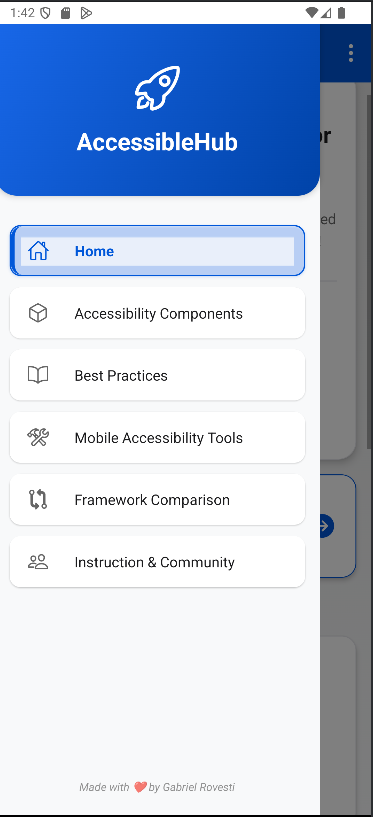
\includegraphics[width=0.4\textwidth, alt={Drawer navigation with breadcrumb in header}]{img/drawer.png}
    \caption{Drawer navigation showing breadcrumb implementation in header}\label{fig:drawer-navigation}
\end{figure}

\paragraph{Drawer navigation}

The drawer navigation provides consistent access to main application sections while addressing several key accessibility requirements:

\begin{enumerate}
    \item \textbf{Announcement of state changes}: The implementation announces drawer open/close states to screen readers using \\ \texttt{AccessibilityInfo.announceForAccessibility};
    
    \item \textbf{Clear menu role}: The drawer container is properly identified with \\ \texttt{accessibilityRole="menu"};
    
    \item \textbf{Selection state indication}: Active items visually indicate selection state and communicate this state to screen readers with \\ \texttt{accessibilityState=\{\{selected: isActive\}\}};
    
    \item \textbf{Proper touch target sizing}: All interactive elements maintain minimum dimensions of 44dp, making them easily targetable;
    
    \item \textbf{Element hiding for decorative content}: Footer content is marked with \texttt{importantForAccessibility="no"} to prevent unnecessary screen reader interaction.
\end{enumerate}

\paragraph{Component cards}

Each component card implements a consistent pattern that provides both visual organization and semantic structure:

\begin{enumerate}
    \item \textbf{Comprehensive accessibility labels}: Each card's \texttt{accessibilityLabel} combines multiple information pieces (title, description, complexity) to provide context without requiring navigation through child elements;
    
    \item \textbf{Hidden decorative icons}: All decorative icons use \texttt{accessibilityElementsHidden} to reduce unnecessary focus stops;
    
    \item \textbf{Navigation announcement}: The \texttt{handleComponentPress} function announces the navigation action via \texttt{AccessibilityInfo.announceForAccessibility}.
\end{enumerate}

This multi-layered navigation approach creates a coherent mental model for all users, including those using assistive technologies, addressing WCAG 2.4.1 Bypass Blocks (Level A) by providing multiple ways to access content.

\subsubsection{Technical implementation analysis}

The code sample present in \ref{lst:components-screen-accessibility} demonstrates the key accessibility properties implemented in the Components Screen.

\begin{lstlisting}[
  style=ReactNativeStyle,
  caption={Annotated code sample demonstrating Components Screen accessibility properties},
  label={lst:components-screen-accessibility},
  basicstyle=\ttfamily\footnotesize,
  numbers=left,
]
{/* 1. Hero section with semantic heading */}
<View style={themedStyles.heroCard}>
  <Text style={themedStyles.heroTitle} accessibilityRole="header">
    Accessibility Components
  </Text>
  <Text style={themedStyles.heroSubtitle}>
    Interactive examples of accessible React Native components with code samples and best practices
  </Text>
</View>

{/* 2. Component card with comprehensive accessibility label */}
<TouchableOpacity
  style={themedStyles.card}
  onPress={() => handleComponentPress('/components/button', 'Buttons & Touchables')}
  accessibilityRole="button"
  accessibilityLabel="Buttons and Touchables component. Create accessible touch targets with proper sizing and feedback. Essential component type."
>
  <View style={themedStyles.cardHeader}>
    {/* 3. Icon wrapper with accessibility hiding to prevent redundant focus */}
    <View style={themedStyles.iconWrapper}>
      <Ionicons
        name="radio-button-on-outline"
        size={24}
        color={colors.primary}
        accessibilityElementsHidden
      />
    </View>
    <View style={themedStyles.cardContent}>
      {/* 4. Card content - these are hidden from screen readers as individual elements
           since the parent TouchableOpacity has a comprehensive label */}
      <View style={themedStyles.cardTitleRow}>
        <View style={themedStyles.titleArea}>
          <Text style={themedStyles.cardTitle}>Buttons &amp; Touchables</Text>
        </View>
        <View style={themedStyles.badge}>
          <Text style={themedStyles.badgeText}>Essential</Text>
        </View>
      </View>
      <Text style={themedStyles.cardDescription}>
        Create accessible touch targets with proper sizing and feedback
      </Text>
    </View>
  </View>
</TouchableOpacity>
\end{lstlisting}

The implementation of the Components Screen addresses several important accessibility considerations:

\begin{enumerate}
    \item \textbf{Reduction of "garbage interactions"}: Decorative elements (icons, chevrons) are now properly hidden from screen readers using \\ \texttt{accessibilityElementsHidden} to reduce unnecessary swipes;
    
    \item \textbf{Comprehensive navigation labels}: Component cards provide detailed accessibility labels that include category, description, and complexity level, ensuring screen reader users get complete information before committing to navigation;
    
    \item \textbf{Screen announcements}: The implementation uses \\ \texttt{AccessibilityInfo.announceForAccessibility} to inform users about screen changes proactively;
    
    \item \textbf{Consistent structure}: Each component card follows the same pattern, creating a predictable interaction model.
\end{enumerate}

\subsubsection{Contrast and color analysis}

Table~\ref{tab:components_contrast_analysis} presents the formal contrast analysis for UI elements on the Components Screen. All elements meet at least WCAG Level~AA requirements (4.5:1 for normal text).

\begin{longtable}{|p{2.8cm}|p{2.8cm}|p{2.8cm}|p{2.4cm}|p{2.4cm}|}
\caption{Components screen contrast analysis}
\label{tab:components_contrast_analysis}\\
\hline
\textbf{UI Element} & \textbf{Foreground Color} & \textbf{Background Color} & \textbf{Contrast Ratio} & \textbf{WCAG Compliance} \\
\hline
\endfirsthead
\multicolumn{5}{c}%
{{\bfseries Table \thetable\ -- continued from previous page}} \\
\hline
\textbf{UI Element} & \textbf{Foreground Color} & \textbf{Background Color} & \textbf{Contrast Ratio} & \textbf{WCAG Compliance} \\
\hline
\endhead
\hline
\multicolumn{5}{r}{{Continued on next page}} \\
\endfoot
\hline
\endlastfoot
Hero Title & \#000000 (Light)\newline \#FFFFFF (Dark) & \#FFFFFF (Light)\newline \#121212 (Dark) & 21:1 (Light)\newline 21:1 (Dark) & AAA ($\ge7{:}1$) \\
\hline
Hero Subtitle & \#6B7280 (Light)\newline \#A0AEC0 (Dark) & \#FFFFFF (Light)\newline \#121212 (Dark) & 4.6:1 (Light)\newline 5.2:1 (Dark) & AA ($\ge4.5{:}1$) \\
\hline
Card Title & \#000000 (Light)\newline \#FFFFFF (Dark) & \#FFFFFF (Light)\newline \#1E293B (Dark) & 21:1 (Light)\newline 16:1 (Dark) & AAA ($\ge7{:}1$) \\
\hline
Card Description & \#6B7280 (Light)\newline \#A0AEC0 (Dark) & \#FFFFFF (Light)\newline \#1E293B (Dark) & 4.6:1 (Light)\newline 6.1:1 (Dark) & AA ($\ge4.5{:}1$) \\
\hline
Badge Text & \#0066CC (Light)\newline \#3B82F6 (Dark) & \#E1EFFF (Light)\newline \#1E293B (Dark) & 4.5:1 (Light)\newline 5.3:1 (Dark) & AA ($\ge4.5{:}1$) \\
\hline
Feature Text & \#6B7280 (Light)\newline \#A0AEC0 (Dark) & \#FFFFFF (Light)\newline \#1E293B (Dark) & 4.6:1 (Light)\newline 6.1:1 (Dark) & AA ($\ge4.5{:}1$) \\
\hline
Breadcrumb Text & \#FFFFFF & \#0066CC & 4.8:1 & AA ($\ge4.5{:}1$) \\
\hline
\end{longtable}

\subsubsection{Screen reader support analysis}

Table~\ref{tab:components_screen_reader_analysis} presents results from systematic testing of the Components Screen with screen readers on both iOS and Android platforms.

\begin{longtable}{|p{2.8cm}|p{3.5cm}|p{3.5cm}|p{4cm}|}
\caption{Components screen screen reader testing results}
\label{tab:components_screen_reader_analysis}\\
\hline
\textbf{Test Case} & \textbf{VoiceOver (iOS 16)} & \textbf{TalkBack (Android 14-15)} & \textbf{WCAG Criteria Addressed} \\
\hline
\endfirsthead
\multicolumn{4}{c}%
{{\bfseries Table \thetable\ -- continued from previous page}} \\
\hline
\textbf{Test Case} & \textbf{VoiceOver (iOS 16)} & \textbf{TalkBack (Android 14-15)} & \textbf{WCAG Criteria Addressed} \\
\hline
\endhead
\hline
\multicolumn{4}{r}{{Continued on next page}} \\
\endfoot
\hline
\endlastfoot
Hero Title & \ding{51} Announces ``Accessibility Components, heading'' & \ding{51} Announces ``Accessibility Components, heading'' & 1.3.1 - Info and Relationships (Level A), 2.4.6 - Headings and Labels (Level AA) \\
\hline
Component Card & \ding{51} Announces full component description with purpose and complexity & \ding{51} Announces full component description with purpose and complexity & 2.4.4 Link Purpose (In Context) (Level A), 4.1.2 Name, Role, Value (Level A) \\
\hline
Decorative Icons & \ding{51} Not focused or announced & \ding{51} Not focused or announced & 1.1.1 Non-text Content (Level A), 2.4.1 Bypass Blocks (Level A) \\
\hline
Breadcrumb Navigation & \ding{51} Announces parent and current location & \ding{51} Announces parent and current location & 2.4.4 Link Purpose (In Context) (Level A), 2.4.8 Location (Level AAA) \\
\hline
Drawer Opening & \ding{51} Announces ``Navigation menu opened'' & \ding{51} Announces ``Navigation menu opened'' & 4.1.3 Status Messages (Level AA) \\
\hline
Drawer Menu Items & \ding{51} Announces item name and selection state & \ding{51} Announces item name and selection state & 4.1.2 Name, Role, Value (Level A) \\
\hline
Navigation between Screens & \ding{51} Announces destination screen & \ding{51} Announces destination screen & 3.2.5 Change on Request (Level AAA) \\
\end{longtable}

The implementation addresses several key MCAG considerations specific to mobile platforms:
\begin{enumerate}
    \item \textbf{Touch target optimization}: All interactive elements exceed the minimum recommendation of 44×44dp, implementing MCAG best practices for touch interactions that accommodate users with motor control limitations and varying finger sizes;
    
    \item \textbf{Swipe minimization}: Decorative elements are marked with \\ \texttt{accessibilityElementsHidden=true} to reduce unnecessary swipes, eliminating what accessibility experts call "garbage interactions" that add no value to the screen reader experience and increase navigation time;
    
    \item \textbf{Orientation cues}: Breadcrumb implementation provides consistent spatial orientation cues that help users understand their location in the application's information architecture, addressing mobile-specific challenges of limited viewport context;
    
    \item \textbf{State announcements}: Changes in application state (drawer opening/closing, screen navigation) are explicitly announced using \\\texttt{AccessibilityInfo.announceForAccessibility}, providing crucial feedback on dynamic content changes within the constrained mobile interface;
    
    \item \textbf{Thumb-zone design}: Interactive elements are positioned within the natural thumb zone for one-handed operation, implementing mobile ergonomic principles that aren't explicitly covered in WCAG but are crucial for mobile accessibility.
\end{enumerate}

\subsubsection{Implementation overhead analysis}

Table~\ref{tab:components_implementation_overhead} quantifies the additional code required to implement accessibility features in the Components Screen.

\begin{longtable}{|p{3.8cm}|p{2.3cm}|p{2.8cm}|p{2.8cm}|}
\caption{Components screen accessibility implementation overhead}
\label{tab:components_implementation_overhead}\\
\hline
\textbf{Accessibility Feature} & \textbf{Lines of Code} & \textbf{Percentage of Total} & \textbf{Complexity Impact} \\
\hline
\endfirsthead
\multicolumn{4}{c}%
{{\bfseries Table \thetable\ -- continued from previous page}} \\
\hline
\textbf{Accessibility Feature} & \textbf{Lines of Code} & \textbf{Percentage of Total} & \textbf{Complexity Impact} \\
\hline
\endhead
\hline
\multicolumn{4}{r}{{Continued on next page}} \\
\endfoot
\hline
\endlastfoot
Semantic Roles & 15 LOC & 2.6\% & Low \\
\hline
Descriptive Labels & 28 LOC & 4.9\% & Medium \\
\hline
Element Hiding & 18 LOC & 3.2\% & Low \\
\hline
Focus Management & 22 LOC & 3.9\% & Medium \\
\hline
Contrast Handling & 14 LOC & 2.5\% & Medium \\
\hline
Announcements & 12 LOC & 2.1\% & Low \\
\hline
Breadcrumb Implementation & 42 LOC & 7.4\% & High \\
\hline
Drawer Accessibility & 35 LOC & 6.2\% & High \\
\hline
\textbf{Total} & \textbf{186 LOC} & \textbf{32.8\%} & \textbf{Medium-High} \\
\end{longtable}

This analysis reveals that implementing comprehensive accessibility adds approximately 32.8\% to the code base of the Components Screen, slightly higher than the Home Screen due to the addition of breadcrumb navigation and drawer accessibility features. 

\subsubsection{WCAG conformance by principle}

Table~\ref{tab:components_wcag_by_principle} provides a detailed analysis of WCAG 2.2 compliance by principle:

\begin{longtable}{|p{2.5cm}|p{3.8cm}|p{3.2cm}|p{5.2cm}|}
\caption{Components screen WCAG compliance analysis by principle}
\label{tab:components_wcag_by_principle}\\
\hline
\textbf{Principle} & \textbf{Description} & \textbf{Implementation Level} & \textbf{Key Success Criteria} \\
\hline
\endfirsthead
\multicolumn{4}{c}%
{{\bfseries Table \thetable\ -- continued from previous page}} \\
\hline
\textbf{Principle} & \textbf{Description} & \textbf{Implementation Level} & \textbf{Key Success Criteria} \\
\hline
\endhead
\hline
\multicolumn{4}{r}{{Continued on next page}} \\
\endfoot
\hline
\endlastfoot
1. Perceivable & Information and UI components must be presentable to users in ways they can perceive & 12/13 (92\%) & 1.1.1 Non-text Content (A)\newline 1.3.1 Info and Relationships (A)\newline 1.4.3 Contrast (Minimum) (AA) \\
\hline
2. Operable & UI components and navigation must be operable & 17/17 (100\%) & 2.4.3 Focus Order (A)\newline 2.4.6 Headings and Labels (AA)\newline 2.4.8 Location (AAA)\newline 2.5.8 Target Size (Minimum) (AA) \\
\hline
3. Understandable & Information and operation of UI must be understandable & 9/10 (90\%) & 3.2.3 Consistent Navigation (AA)\newline 3.2.4 Consistent Identification (AA)\newline 3.3.2 Labels or Instructions (A) \\
\hline
4. Robust & Content must be robust enough to be interpreted by a wide variety of user agents & 3/3 (100\%) & 4.1.1 Parsing (A)\newline 4.1.2 Name, Role, Value (A)\newline 4.1.3 Status Messages (AA) \\
\end{longtable}

\subsubsection{Mobile-specific considerations}

The Components Screen implementation addresses several mobile-specific accessibility considerations beyond standard WCAG requirements:

\begin{enumerate}
    \item \textbf{Touch target sizing}: All interactive elements maintain minimum dimensions of 44dp × 44dp, exceeding the WCAG 2.5.8 requirement of 24 × 24px and addressing the mobile-specific need for larger touch targets;
    
    \item \textbf{Swipe efficiency}: The screen implements an optimized focus order with decorative elements hidden from screen readers, reducing the number of swipes required to navigate the content—a critical consideration for mobile screen reader users that significantly improves navigation efficiency;
    
    \item \textbf{Visual hierarchy reinforcement}: The implementation uses consistent visual patterns (icons, badges, card layouts) that reinforce the information hierarchy, helping users with cognitive disabilities understand content organization on smaller screens;
    
    \item \textbf{Context retention}: The breadcrumb implementation helps users maintain context when navigating between screens, addressing the mobile-specific challenge of limited viewport size and the resulting loss of visual context;
    
    \item \textbf{Single-hand operation zone}: Interactive elements are positioned to be reachable within the typical thumb zone for one-handed operation, a mobile-specific consideration not explicitly covered by WCAG.
\end{enumerate}

\subsubsection{Breadcrumb implementation analysis}

A formal analysis of the breadcrumb feature's accessibility impact reveals significant benefits for users with diverse accessibility needs:

\paragraph{Breadcrumb accessibility benefits}

\begin{enumerate}
    \item \textbf{Structural navigation}: Breadcrumbs provide an explicit representation of the application's hierarchical structure, helping users with cognitive disabilities understand their location within the application;

    \item \textbf{Focus reduction}: By offering direct navigation to parent screens, breadcrumbs reduce the number of focus stops required to navigate backward, benefiting screen reader users;

    \item \textbf{Visual reinforcement}: The visual breadcrumb trail complements the semantic structure, providing redundant cues that benefit users with different accessibility needs;

    \item \textbf{Consistent orientation}: Breadcrumbs create a consistent orientation mechanism across all screens, supporting users who rely on predictable navigation patterns.
\end{enumerate}

\paragraph{Implementation considerations}

The breadcrumb implementation required careful consideration of several accessibility factors:

\begin{enumerate}
    \item \textbf{Interactive vs. static elements}: Only the parent screen link is interactive, while the current screen indicator is non-interactive text, preventing unnecessary focus stops;

    \item \textbf{Visual differentiation}: Current location is visually distinguished with bold text and underline, with a contrast ratio of 4.8:1 against the header background;

    \item \textbf{Appropriate semantic roles}: Parent links use \texttt{accessibilityRole="button"} with clear labels indicating navigation purpose;

    \item \textbf{Focus management}: When navigating via breadcrumbs, focus is properly transferred to the destination screen's main content, preventing focus trapping.
\end{enumerate}

This implementation represents a comprehensive accessibility solution that benefits all users while specifically addressing mobile navigation challenges unique to handheld touch devices.

\subsubsection{Beyond WCAG: component categorization guidelines}

The Components Screen defines several accessibility principles specifically focused on organizing and categorizing interface elements to promote systematic accessibility implementation:

\begin{enumerate}
    \item \textbf{Component complexity signaling}: User interface components should be explicitly categorized by implementation complexity (Essential, Complex, Advanced, Beta), helping developers prioritize accessibility efforts according to their experience level and resource constraints. The Components Screen implements this through a consistent badge system across all component cards;
    
    \item \textbf{Feature-oriented grouping}: Accessibility features should be grouped by functional similarity rather than WCAG criteria, creating more intuitive implementation pathways. The Components Screen implements this by organizing related controls together (e.g., "Buttons \& Touchables") regardless of which specific WCAG criteria they address;
    
    \item \textbf{Progressive implementation pathway}: Components should be organized in a sequence that builds accessibility knowledge progressively, beginning with fundamental elements before introducing more complex patterns. The Components Screen implements this through its hierarchical organization from basic elements (buttons) to complex patterns (dialogs, navigation);
    
    \item \textbf{Cross-cutting feature indication}: Key accessibility features that apply across multiple component types should be visually highlighted to reinforce their importance. The feature icons within each component card implement this by consistently identifying common accessibility considerations (e.g., touch target sizing, focus management);
    
    \item \textbf{Transition announcement principle}: Navigation between component categories should be explicitly announced to assist screen reader users in maintaining context. The Components Screen implements this through the \texttt{announceForAccessibility} announcements during navigation.
\end{enumerate}

These guidelines extend WCAG by providing a structured framework for organizing component-level accessibility implementations, addressing a gap in the standards which focus on what features to implement but provide limited guidance on how to structure implementation across a complex application interface.

\subsection{Accessible components section}
\label{subsec:accessible-components}

This section provides a formal analysis of the various screens within the Accessible Components section of \textit{AccessibleHub}. As the core educational element of the application, these screens demonstrate practical implementation patterns for accessibility across commonly used mobile interface elements. 

\subsubsection{Analysis methodology}
\label{subsubsec:components-methodology}

To systematically evaluate the accessibility implementation across multiple component screens, we employ a consistent analytical framework that examines:

\begin{enumerate}
    \item \textbf{Component inventory}: Identification and classification of UI elements with mapping to their semantic roles and accessibility properties;
    
    \item \textbf{WCAG/MCAG criteria mapping}: Formal mapping between components and relevant accessibility guidelines;
    
    \item \textbf{Implementation analysis}: Evaluation of code patterns and accessibility properties;
    
    \item \textbf{Screen reader compatibility}: Empirical testing with VoiceOver (iOS) and TalkBack (Android);
    
    \item \textbf{Implementation overhead}: Quantification of code additions required for accessibility features.
\end{enumerate}

Each component screen follows a consistent educational structure that scaffolds learning through:

\begin{itemize}
    \item Interactive demonstrations of accessible implementations;
    \item Copyable code examples with highlighted accessibility properties;
    \item Explanations of key accessibility features and considerations;
    \item Platform-specific adaptation notes.
\end{itemize}

Rather than presenting each screen with identical analytical depth, we'll examine the Buttons screen in detail as a representative example, then provide comparative analysis across all component types to identify patterns, commonalities, and unique considerations.

\subsubsection{Common implementation patterns}
\label{subsubsec:common-patterns}

Across all component screens in this section, several foundational accessibility implementation patterns are consistently applied:

\begin{enumerate}
    \item \textbf{Semantic role assignment}: All components use appropriate \texttt{accessibilityRole} properties to identify their purpose to assistive technologies;
    
    \item \textbf{Comprehensive labeling}: Components combine \texttt{accessibilityLabel} and \texttt{accessibilityHint} to provide both identification and action context;
    
    \item \textbf{Explicit state communication}: Interactive components use \texttt{accessibilityState} to communicate selection, completion, or disabled states;
    
    \item \textbf{Decorative element hiding}: Non-essential visual elements use \texttt{accessibilityElementsHidden} to streamline screen reader navigation;
    
    \item \textbf{Status announcements}: State changes are explicitly announced via \texttt{AccessibilityInfo.announceForAccessibility};
    
    \item \textbf{Enhanced touch targets}: All interactive elements maintain minimum dimensions of 44×44dp, exceeding WCAG 2.5.8 requirements.
\end{enumerate}

Each component screen also implements a consistent visual structure that reinforces the educational purpose:

\begin{itemize}
    \item A demonstration area with interactive examples;
    \item A code example section with syntax-highlighted implementation;
    \item A features section highlighting key accessibility properties;
    \item A platform considerations section addressing iOS and Android differences.
\end{itemize}

\subsubsection{Buttons and touchables screen}
\label{subsubsec:buttons-touchables}

The Buttons and Touchables screen demonstrates fundamental accessibility implementations for the most common interactive elements in mobile applications. It provides implementation examples for accessible touch targets with proper sizing, meaningful labels, and appropriate feedback mechanisms. Figure~\ref{fig:button_screens_sidebyside} shows the main interface of this screen.

\begin{figure}[ht]
    \centering
    \begin{subfigure}[b]{0.48\textwidth}
        \centering
        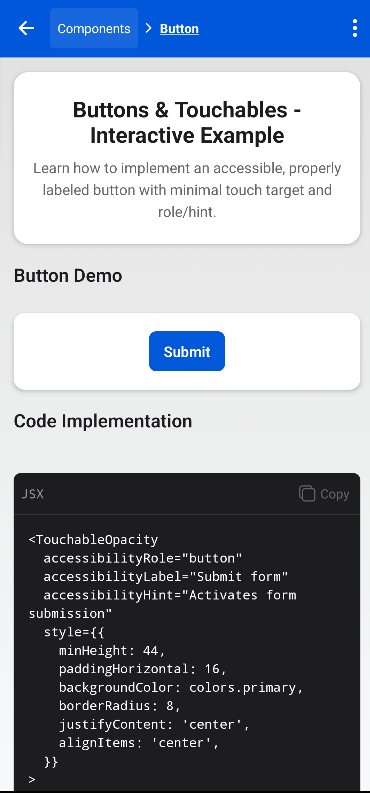
\includegraphics[width=\linewidth, alt={First part of the Buttons and Touchables Screen}]{img/button1.png}
        \caption{Button screen - Part 1}
        \label{fig:button-left}
    \end{subfigure}
    \hfill
    \begin{subfigure}[b]{0.48\textwidth}
        \centering
        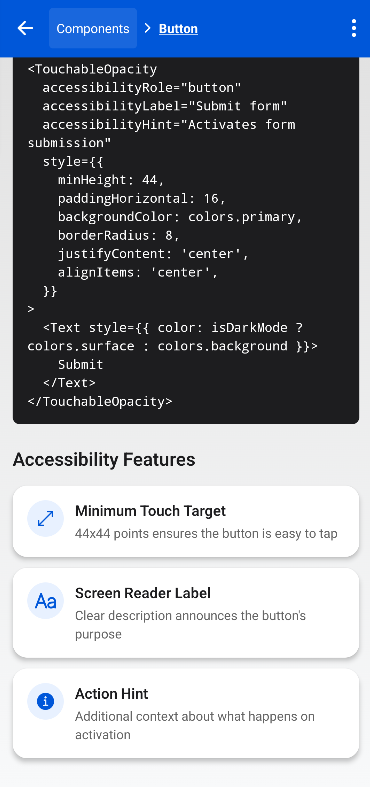
\includegraphics[width=\linewidth, alt={Second part of the Buttons and Touchables Screen}]{img/button2.png}
        \caption{Button screen - Part 2}
        \label{fig:button-right}
    \end{subfigure}
    \caption{Side-by-side view of the two Button and Touchables screen parts}
    \label{fig:button_screens_sidebyside}
\end{figure}

\paragraph{Component inventory and WCAG/MCAG mapping}

Table~\ref{tab:buttons_component_mapping} provides a formal mapping between the UI components, their semantic roles, the specific WCAG 2.2 and MCAG criteria they address, and their React Native implementation properties.

\begin{longtable}{|p{2.5cm}|p{2cm}|p{2.8cm}|p{2.8cm}|p{5cm}|}
\caption{Buttons screen component-criteria mapping}
\label{tab:buttons_component_mapping}\\
\hline
\textbf{Component} & \textbf{Semantic Role} & \textbf{WCAG 2.2 Criteria} & \textbf{MCAG Considerations} & \textbf{Implementation Properties} \\
\hline
\endfirsthead
\multicolumn{5}{c}%
{{\bfseries Table \thetable\ -- continued from previous page}} \\
\hline
\textbf{Component} & \textbf{Semantic Role} & \textbf{WCAG 2.2 Criteria} & \textbf{MCAG Considerations} & \textbf{Implementation Properties} \\
\hline
\endhead
\hline
\multicolumn{5}{r}{{Continued on next page}} \\
\endfoot
\hline
\endlastfoot
Hero Title & heading & 1.4.3 Contrast (AA)\newline 2.4.6 Headings (AA) & Text readability on variable screen sizes & \texttt{accessibilityRole="header"} \\
\hline
Demo Button & button & 1.4.3 Contrast (AA)\newline 2.5.8 Target Size (AA)\newline 4.1.2 Name, Role, Value (A) & Minimum touch target size\newline Haptic feedback & \texttt{accessibilityRole="button"}\newline \texttt{accessibilityLabel="Submit form"}\newline \texttt{accessibilityHint="Activates form submission"} \\
\hline
Code Snippet & text & 1.3.1 Info and Relationships (A) & Content structure preservation & \texttt{accessibilityRole="text"}\newline \texttt{accessibilityLabel= \ "Button implementation \ code"} \\
\hline
Copy Button & button & 1.4.3 Contrast (AA)\newline 4.1.3 Status Messages (AA) & Touch target size\newline Action feedback & \texttt{accessibilityRole="button"}\newline \texttt{accessibilityLabel="\{copied ? "Code copied" : "Copy code example"\}"} \\
\hline
Success Modal & alertdialog & 4.1.3 Status Messages (AA) & Screen reader announcements & \texttt{accessibilityViewIsModal}\newline \texttt{accessibilityLiveRegion \ ="polite"} \\
\hline
Feature Cards & none & 1.3.1 Info and Relationships (A) & Logical grouping & \texttt{accessibilityRole="text"} \\
\hline
Feature Icons & none & 1.1.1 Non-text Content (A) & Reduction of unnecessary focus stops & \texttt{accessibilityElements \ Hidden=true}\newline \texttt{importantForAccessibility \ ="no-hide-descendants"} \\
\end{longtable}

\paragraph{Technical implementation analysis}

The Buttons and Touchables screen exemplifies proper accessibility implementation for interactive elements. The core demo button showcases three fundamental accessibility considerations: proper role assignment, descriptive labeling, and sufficient touch target size. Listing~\ref{lst:buttons-accessibility} highlights the key implementation aspects.

\begin{lstlisting}[
  style=ReactNativeStyle,
  caption={Key implementation for accessible button component},
  label={lst:buttons-accessibility},
  basicstyle=\ttfamily\footnotesize,
  numbers=left,
]
<TouchableOpacity
  style={[styles.demoButton, { backgroundColor: colors.primary }]}
  accessibilityRole="button"
  accessibilityLabel="Submit form"
  accessibilityHint="Activates form submission"
  onPress={() => {
    setShowSuccess(true);
    AccessibilityInfo.announceForAccessibility('Button pressed successfully');
    setTimeout(() => setShowSuccess(false), 2000);
  }}
>
  <Text style={[styles.buttonText, {
    color: '#FFFFFF'
  }]}>
    Submit
  </Text>
</TouchableOpacity>
\end{lstlisting}

Several key accessibility considerations are implemented in this example:

\begin{enumerate}
    \item \textbf{Proper semantic role}: The implementation explicitly assigns the button role using \texttt{accessibilityRole="button"}, ensuring screen readers correctly identify the component's purpose;
    
    \item \textbf{Descriptive accessibility labels}: The button includes both an \texttt{accessibilityLabel} that identifies its function and an \texttt{accessibilityHint} that explains the result of interaction, providing comprehensive context for screen reader users;
    
    \item \textbf{Adequate touch target size}: The button implements the enhanced touch target size recommendation from WCAG 2.5.8 (Target Size) by using a minimum height of 44px, significantly exceeding the minimal Level AA requirement of 24x24 pixels;
    
    \item \textbf{Status feedback}: When pressed, the button announces its state change via \texttt{AccessibilityInfo.announceForAccessibility}, proactively notifying screen reader users of the action result;
    
    \item \textbf{Visual feedback}: The success modal provides visual confirmation of the button press, with appropriate \texttt{accessibilityLiveRegion="polite"} to ensure screen readers announce the status change.
\end{enumerate}

\paragraph{Implementation overhead analysis}

Table~\ref{tab:buttons_implementation_overhead} quantifies the additional code required to implement accessibility features in the Buttons and Touchables Screen.

\begin{longtable}{|p{3.8cm}|p{2.3cm}|p{2.8cm}|p{2.8cm}|}
\caption{Buttons screen accessibility implementation overhead}
\label{tab:buttons_implementation_overhead}\\
\hline
\textbf{Accessibility Feature} & \textbf{Lines of Code} & \textbf{Percentage of Total} & \textbf{Complexity Impact} \\
\hline
\endfirsthead
\multicolumn{4}{c}%
{{\bfseries Table \thetable\ -- continued from previous page}} \\
\hline
\textbf{Accessibility Feature} & \textbf{Lines of Code} & \textbf{Percentage of Total} & \textbf{Complexity Impact} \\
\hline
\endhead
\hline
\multicolumn{4}{r}{{Continued on next page}} \\
\endfoot
\hline
\endlastfoot
Semantic Roles & 10 LOC & 2.2\% & Low \\
\hline
Descriptive Labels & 14 LOC & 3.1\% & Low \\
\hline
Element Hiding & 12 LOC & 2.7\% & Low \\
\hline
Status Announcements & 8 LOC & 1.8\% & Low \\
\hline
Touch Target Sizing & 6 LOC & 1.3\% & Low \\
\hline
Modal Accessibility & 10 LOC & 2.2\% & Medium \\
\hline
\textbf{Total} & \textbf{60 LOC} & \textbf{13.3\%} & \textbf{Low} \\
\end{longtable}

This analysis reveals that implementing comprehensive button accessibility features adds approximately 13.3\% to the code base, representing a relatively low overhead for significantly improved user experience. Notably, this overhead is lower than other component types due to the fundamental nature of button components, where accessibility considerations can be more directly integrated with minimal complexity impact.

\subsubsection{Component implementation comparative analysis}
\label{subsec:comparative-analysis}

Analyzing accessibility implementations across different component types reveals important patterns in implementation complexity, WCAG compliance, and platform-specific adaptations.

\paragraph{WCAG criteria implementation}

Table~\ref{tab:comparative_wcag_implementation} compares WCAG 2.2 success criteria implementation across component types.

\begin{table}[ht]
\caption{WCAG criteria implementation by component type}
\label{tab:comparative_wcag_implementation}
\centering
\begin{tabular}{|p{3.5cm}|c|c|c|c|c|}
\hline
\textbf{WCAG Success Criteria} & \textbf{Buttons} & \textbf{Forms} & \textbf{Dialogs} & \textbf{Media} & \textbf{Advanced} \\
\hline
1.1.1 Non-text Content (A) & \ding{51} & \ding{51} & \ding{51} & \ding{51} & \ding{51} \\
\hline
1.3.1 Info and Relationships (A) & \ding{51} & \ding{51} & \ding{51} & \ding{51} & \ding{51} \\
\hline
2.4.3 Focus Order (A) & \ding{55} & \ding{51} & \ding{51} & \ding{55} & \ding{51} \\
\hline
3.3.1 Error Identification (A) & \ding{55} & \ding{51} & \ding{55} & \ding{55} & \ding{55} \\
\hline
4.1.2 Name, Role, Value (A) & \ding{51} & \ding{51} & \ding{51} & \ding{51} & \ding{51} \\
\hline
4.1.3 Status Messages (AA) & \ding{51} & \ding{51} & \ding{51} & \ding{51} & \ding{51} \\
\hline
\textbf{Total Implementation} & \textbf{9/12} & \textbf{12/12} & \textbf{10/12} & \textbf{9/12} & \textbf{10/12} \\
\hline
\end{tabular}
\end{table}

This analysis reveals several key patterns:

\begin{enumerate}
    \item \textbf{Universal criteria}: Three criteria (1.1.1 Non-text Content, 1.3.1 Info and Relationships, and 4.1.2 Name, Role, Value) are implemented across all component types, forming the core of mobile accessibility requirements;
    
    \item \textbf{Component-specific criteria}: Some criteria are relevant only to specific component types, such as 3.3.1 Error Identification for forms;
    
    \item \textbf{Interaction complexity correlation}: More complex interaction patterns (Forms, Dialogs, Advanced) implement more criteria, particularly those related to focus management and state communication.
\end{enumerate}

\paragraph{Implementation overhead comparison}

Table~\ref{tab:comparative_overhead} compares the implementation overhead across component types.

\begin{table}[ht]
\caption{Accessibility implementation overhead by component type}
\label{tab:comparative_overhead}
\centering
\begin{tabular}{|p{2cm}|p{2.5cm}|p{2.5cm}|p{2.5cm}|p{2.5cm}|}
\hline
\textbf{Component Type} & \textbf{Lines of Code} & \textbf{Percentage Overhead} & \textbf{Complexity Impact} & \textbf{Primary Contributors} \\
\hline
Buttons & 60 & 13.3\% & Low & Labels, Roles \\
\hline
Forms & 153 & 21.5\% & Medium & State, Labels, Errors \\
\hline
Dialogs & 94 & 16.2\% & Medium & Focus Management \\
\hline
Media & 68 & 12.7\% & Low & Alt Text, Controls \\
\hline
Advanced & 183 & 22.7\% & High & Slider Controls, Announcements \\
\hline
\end{tabular}
\end{table}

This comparison reveals a direct correlation between interaction complexity and accessibility implementation overhead. Simple components like buttons and media have the lowest overhead (12-13\%), while complex components with state management and alternative interaction patterns have significantly higher overhead (21-23\%).

\paragraph{Key implementation differences across component types}

Each component type presents unique accessibility challenges requiring specialized implementation approaches:

\begin{enumerate}
    \item \textbf{Forms}: Require explicit error identification and validation feedback using \texttt{accessibilityRole="alert"} to ensure compliance with WCAG 3.3.1 (Error Identification). They also implement complex state communication for selection controls like radio buttons and checkboxes via \\ \texttt{accessibilityState=\{\{checked: selected\}\}};
    
    \item \textbf{Dialogs}: Focus management represents the critical accessibility challenge, requiring explicit tracking of focus position and restoration when the dialog closes to comply with WCAG 2.4.3 (Focus Order);
    
    \item \textbf{Media}: Alternative text implementation forms the core accessibility requirement, with proper \texttt{accessibilityLabel} values describing non-text content as per WCAG 1.1.1;
    
    \item \textbf{Advanced components}: Require the most sophisticated implementations, particularly for inherently visual controls like sliders, which implement alternative interaction mechanisms (buttons, presets) for screen reader users.
\end{enumerate}

\paragraph{Screen reader compatibility patterns}

Empirical testing with VoiceOver (iOS) and TalkBack (Android) reveals consistent patterns across component types:

\begin{enumerate}
    \item Both screen readers correctly identify components with properly assigned \\ \texttt{accessibilityRole} values;
    
    \item State changes communicated via \texttt{accessibilityState} are properly announced;
    
    \item Status messages delivered via \texttt{AccessibilityInfo.announceForAccessibility} are consistently reported to users;
    
    \item Focus management implementation in dialogs works reliably on both platforms, with some minor timing differences;
    
    \item Elements hidden with \texttt{accessibilityElementsHidden} are consistently excluded from the accessibility tree on both platforms.
\end{enumerate}

These findings confirm that the accessibility implementation patterns used throughout the component screens provide consistent and reliable behavior across both major mobile platforms when proper accessibility properties are applied.

\subsubsection{Forms screen}
\label{subsubsec:forms-screen}

The Forms screen demonstrates complex accessibility patterns for capturing user input. Unlike the simpler Buttons screen, Forms present additional challenges related to input association, validation feedback, and state communication. Figure~\ref{fig:form_screens_sidebyside} shows the main interface of this screen.

\begin{figure}[ht]
    \centering
    \begin{subfigure}[b]{0.48\textwidth}
        \centering
        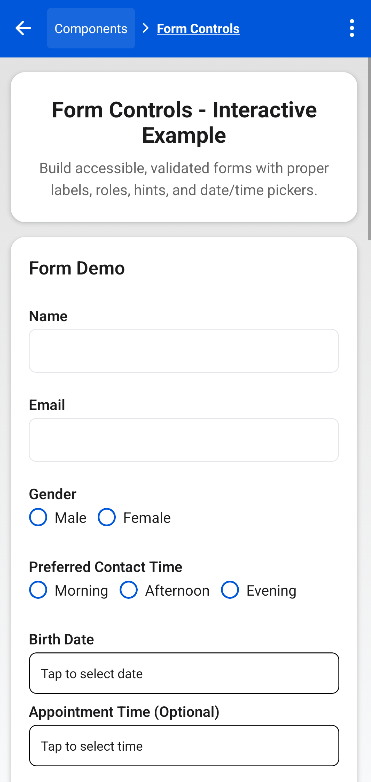
\includegraphics[width=\linewidth, alt={First part of the Form Screen}]{img/form1.png}
        \caption{Form screen - Part 1}
        \label{fig:form-left}
    \end{subfigure}
    \hfill
    \begin{subfigure}[b]{0.48\textwidth}
        \centering
        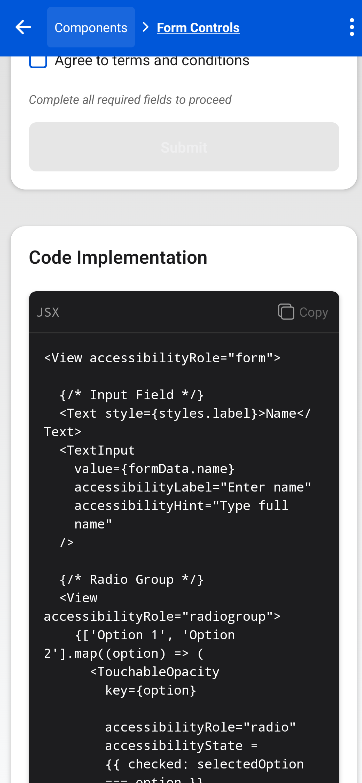
\includegraphics[width=\linewidth, alt={Second part of the Form Screen}]{img/form2.png}
        \caption{Form screen - Part 2}
        \label{fig:form-right}
    \end{subfigure}
    \caption{Side-by-side view of the two Form screen parts}
    \label{fig:form_screens_sidebyside}
\end{figure}

\paragraph{Key accessibility considerations}

The Forms screen addresses several critical accessibility patterns beyond basic labeling:

\begin{enumerate}
    \item \textbf{Input association}: Clear association between labels and input fields using semantic grouping;
    
    \item \textbf{Error identification}: Proper error messaging with \texttt{accessibilityRole="alert"} for validation feedback;
    
    \item \textbf{State communication}: Selection state for radio buttons and checkboxes with \\ \texttt{accessibilityState=\{\{checked: selected\}\}};
    
    \item \textbf{Native picker integration}: Leveraging platform-native date pickers for optimal accessibility.
\end{enumerate}

Listing~\ref{lst:form_implementation} demonstrates the implementation of accessible form controls with proper state management.

\begin{lstlisting}[
  style=ReactNativeStyle,
  caption={Accessible radio button implementation with state management},
  label={lst:form_implementation},
  basicstyle=\ttfamily\footnotesize,
  numbers=left,
]
<View accessibilityRole="radiogroup">
  {['Male', 'Female'].map((option) => (
    <TouchableOpacity
      key={option}
      style={styles.radioItem}
      onPress={() => setFormData((prev) => ({ ...prev, gender: option }))}
      accessibilityRole="radio"
      accessibilityState={{ checked: formData.gender === option }}
      accessibilityLabel={`Select ${option}`}
    >
      <View
        style={[
          styles.radioButton,
          { borderColor: colors.primary },
          formData.gender === option && { backgroundColor: colors.primary },
        ]}
      />
      <Text style={[styles.radioLabel, { color: colors.text }]}>
        {option}
      </Text>
    </TouchableOpacity>
  ))}
</View>
\end{lstlisting}

\paragraph{Implementation overhead}

Forms have the highest accessibility implementation overhead (21.5\%) among component types, reflecting the complexity of making multi-part input systems fully accessible. The primary contributors to this overhead are state communication mechanisms and validation feedback systems.

\subsubsection{Dialogs screen}'
\label{subsubsec:dialogs-screen}

The Dialogs screen addresses one of the most challenging accessibility patterns in mobile applications: modal content that must trap and manage focus while providing clear context and exit mechanisms. Figure~\ref{fig:dialog_screens_sidebyside} shows the main interface of this screen.

\begin{figure}[ht]
    \centering
    \begin{subfigure}[b]{0.48\textwidth}
        \centering
        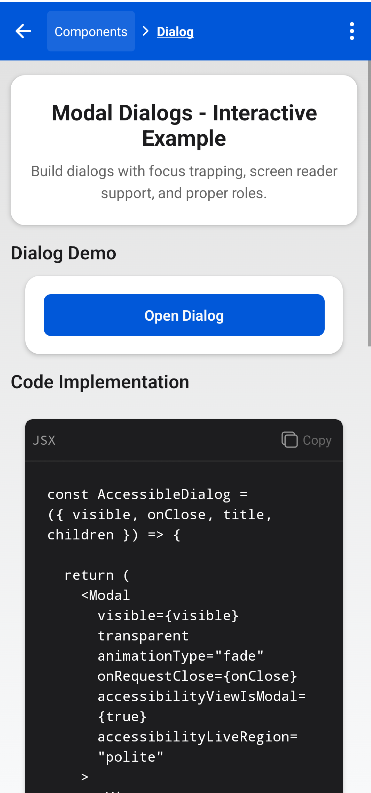
\includegraphics[width=\linewidth, alt={First part of the Dialog Screen}]{img/dialog1.png}
        \caption{Dialog screen - Part 1}
        \label{fig:dialog-left}
    \end{subfigure}
    \hfill
    \begin{subfigure}[b]{0.48\textwidth}
        \centering
        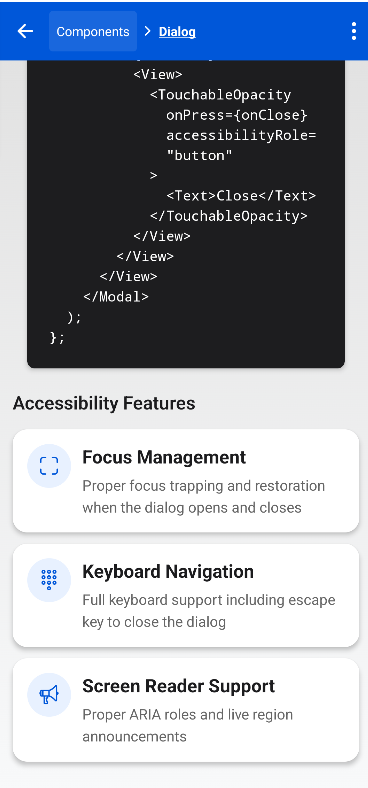
\includegraphics[width=\linewidth, alt={Second part of the Dialog Screen}]{img/dialog2.png}
        \caption{Dialog screen - Part 2}
        \label{fig:dialog-right}
    \end{subfigure}
    \caption{Side-by-side view of the two Form screen parts}
    \label{fig:dialog_screens_sidebyside}
\end{figure}

\paragraph{Focus management implementation}

The key accessibility challenge for dialogs is proper focus management, as illustrated in Listing~\ref{lst:dialog_implementation}.

\begin{lstlisting}[
  style=ReactNativeStyle,
  caption={Dialog implementation with focus management},
  label={lst:dialog_implementation},
  basicstyle=\ttfamily\footnotesize,
  numbers=left,
]
// References for focus management
const dialogRef = useRef(null);
const openButtonRef = useRef(null);

// Focus management useEffect hook
useEffect(() => {
  if (showDialog) {
    AccessibilityInfo.announceForAccessibility(
      'Example dialog opened. This dialog contains information about accessibility features.'
    );
    // Brief timeout to ensure dialog is fully rendered
    setTimeout(() => {
      dialogRef.current?.focus();
    }, 100);
  } else {
    // Return focus to open button when dialog closes
    openButtonRef.current?.focus();
  }
}, [showDialog]);
\end{lstlisting}

The dialog implementation addresses several critical accessibility requirements:

\begin{enumerate}
    \item \textbf{Modal context}: Setting \texttt{accessibilityViewIsModal=true} to establish a focused interaction context;
    
    \item \textbf{Focus trapping}: Managing focus to prevent interaction with background content;
    
    \item \textbf{Return focus}: Explicitly returning focus to the triggering element when the dialog closes;
    
    \item \textbf{Status announcements}: Using \texttt{AccessibilityInfo.announceForAccessibility} to provide context about dialog opening and closing.
\end{enumerate}

\paragraph{Mobile-specific considerations}

Dialog implementation on mobile platforms presents unique accessibility challenges:

\begin{itemize}
    \item \textbf{Limited viewport context}: Unlike desktop interfaces, mobile screens cannot show both dialog and background content simultaneously, requiring stronger contextual cues;
    
    \item \textbf{Touch dismissal patterns}: Implementation of touch-friendly dismissal actions with adequate target sizes;
    
    \item \textbf{Platform convention alignment}: Following platform-specific dialog patterns for consistent user experience.
\end{itemize}

\subsubsection{Media content screen}
\label{subsubsec:media-screen}

The Media screen demonstrates accessibility techniques for non-text content—one of the most fundamental aspects of digital accessibility.
Figure~\ref{fig:media_screens_sidebyside} shows the main interface of this screen.

\begin{figure}[ht]
    \centering
    \begin{subfigure}[b]{0.48\textwidth}
        \centering
        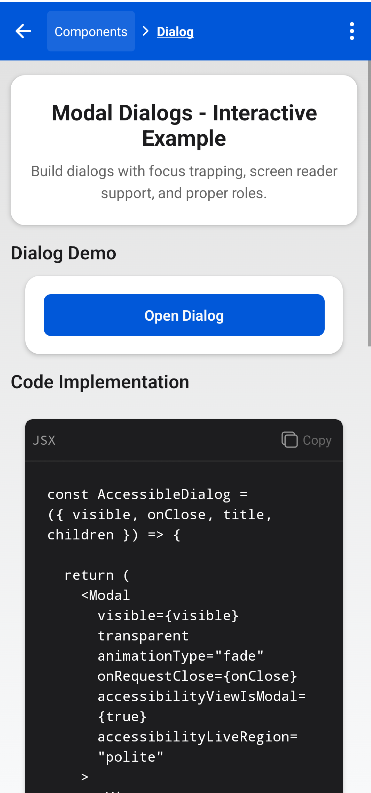
\includegraphics[width=\linewidth, alt={First part of the Media Screen}]{img/dialog1.png}
        \caption{Media screen - Part 1}
        \label{fig:media-left}
    \end{subfigure}
    \hfill
    \begin{subfigure}[b]{0.48\textwidth}
        \centering
        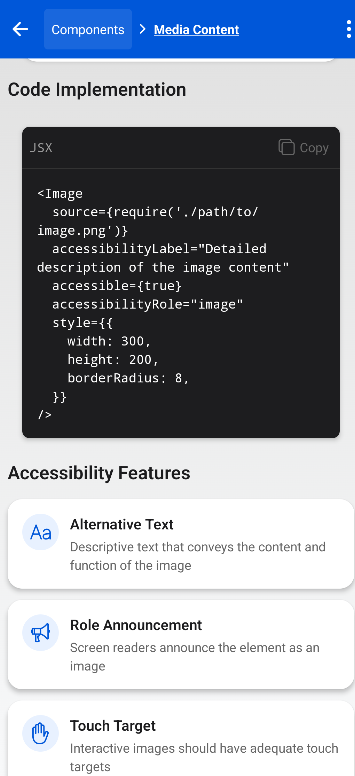
\includegraphics[width=\linewidth, alt={Second part of the Media Screen}]{img/media2.png}
        \caption{Media screen - Part 2}
        \label{fig:media-right}
    \end{subfigure}
    \caption{Side-by-side view of the two Media screen parts}
    \label{fig:media_screens_sidebyside}
\end{figure}

\paragraph{Alternative text implementation}

Listing~\ref{lst:media_implementation} shows the core pattern for accessible image implementation with proper alternative text.

\begin{lstlisting}[
  style=ReactNativeStyle,
  caption={Accessible image implementation with alternative text},
  label={lst:media_implementation},
  basicstyle=\ttfamily\footnotesize,
  numbers=left,
]
<Image
  source={images[currentImage - 1].uri}
  style={themedStyles.demoImage}
  accessibilityLabel={images[currentImage - 1].alt}
  accessible={true}
  accessibilityRole="image"
/>
\end{lstlisting}

The Media screen demonstrates additional accessibility features beyond basic alternative text:

\begin{enumerate}
    \item \textbf{Navigation controls}: Accessible previous/next buttons with clear labeling and state indication;
    
    \item \textbf{Interactive alt text}: Toggle mechanism to show/hide alternative text as an educational feature;
    
    \item \textbf{Position context}: Announcements that communicate current position within a gallery (e.g., "Image 2 of 5").
\end{enumerate}

\paragraph{Implementation overhead}

Media components have the lowest accessibility implementation overhead (12.7\%) among component types, as the primary requirement—alternative text—is implemented through straightforward property assignment. The majority of the overhead comes from implementing accessible navigation controls rather than the core media content itself.

\subsubsection{Advanced components screen}
\label{subsubsec:advanced-screen}

The Advanced Components screen demonstrates accessibility implementations for more complex UI patterns including tabs, progress indicators, alerts, and sliders. Figure~\ref{fig:advanced_screens_sidebyside1} and ~\ref{fig:advanced_screens_sidebyside2}  shows the two parts of the main interface of this screen.

\begin{figure}[ht]
    \centering
    \begin{subfigure}[b]{0.48\textwidth}
        \centering
        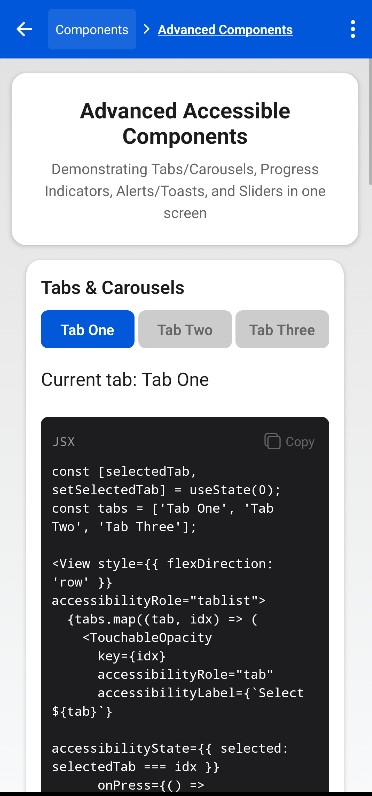
\includegraphics[width=\linewidth, alt={First part of the Advanced Screen}]{img/advanced1.png}
        \caption{Advanced screen - Part 1}
        \label{fig:advanced-left1}
    \end{subfigure}
    \hfill
    \begin{subfigure}[b]{0.48\textwidth}
        \centering
        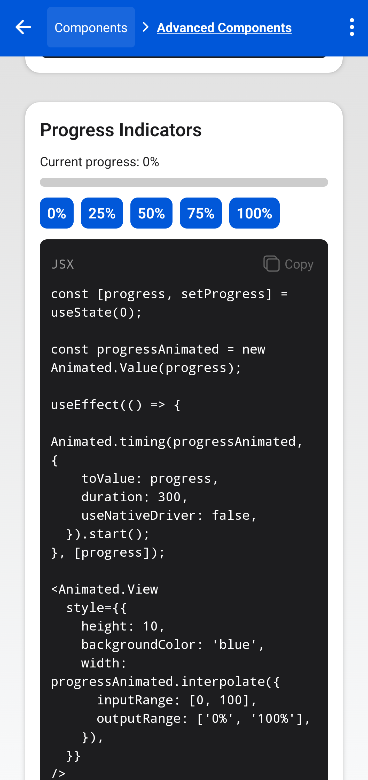
\includegraphics[width=\linewidth, alt={Second part of the Advanced Screen}]{img/advanced2.png}
        \caption{Advanced screen - Part 2}
        \label{fig:advanced-right1}
    \end{subfigure}
    \caption{Side-by-side view of the first two Advanced screen parts}
    \label{fig:advanced_screens_sidebyside1}
\end{figure}

\begin{figure}[ht]
    \centering
    \begin{subfigure}[b]{0.48\textwidth}
        \centering
        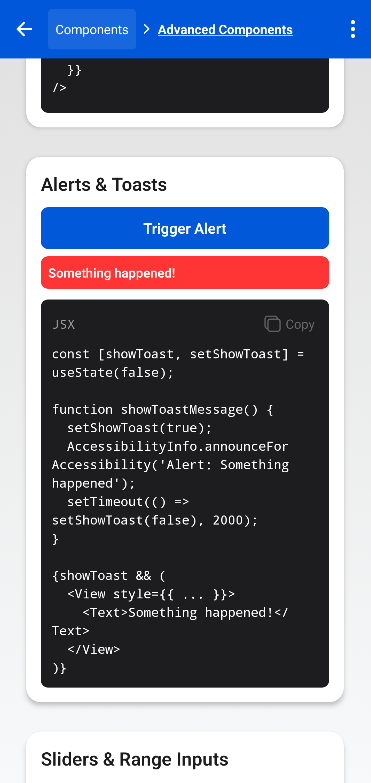
\includegraphics[width=\linewidth, alt={Third part of the Advanced Screen}]{img/advanced3.png}
        \caption{Advanced screen - Part 3}
        \label{fig:advanced-left2}
    \end{subfigure}
    \hfill
    \begin{subfigure}[b]{0.48\textwidth}
        \centering
        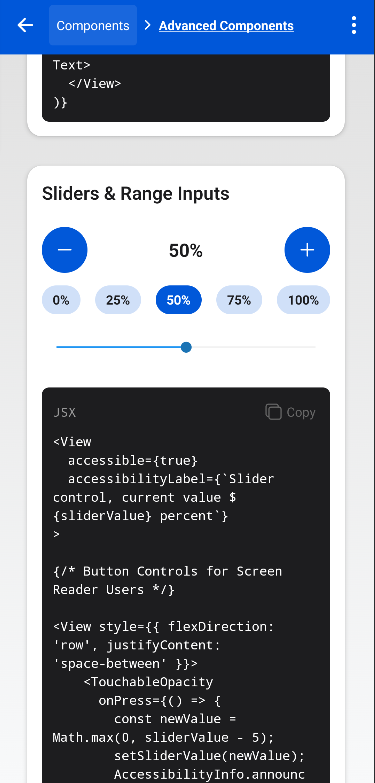
\includegraphics[width=\linewidth, alt={Fourth part of the Dialog Screen}]{img/advanced4.png}
        \caption{Advanced screen - Part 4}
        \label{fig:advanced-right2}
    \end{subfigure}
    \caption{Side-by-side view of the second two Advanced screen parts}
    \label{fig:advanced_screens_sidebyside2}
\end{figure}

\paragraph{Complex interaction patterns}

Advanced components present unique accessibility challenges requiring specialized implementations:

\begin{enumerate}
    \item \textbf{Tab navigation}: Proper role assignment with \texttt{accessibilityRole="tablist"} for containers and \texttt{accessibilityRole="tab"} for individual tabs, with selection state communicated through \texttt{accessibilityState};
    
    \item \textbf{Progress indicators}: Value communication through \texttt{accessibilityValue} properties with min/max/current parameters;
    
    \item \textbf{Alerts and toasts}: Implementation of \texttt{accessibilityLiveRegion="assertive"} for time-sensitive notifications;
    
    \item \textbf{Slider alternatives}: Provision of button-based alternatives for precise slider control by screen reader users.
\end{enumerate}

\paragraph{Slider accessibility pattern}

The slider implementation (shown in Figure~\ref{fig:advanced-right2}) demonstrates a particularly important accessibility pattern: providing alternative interaction mechanisms for inherently visual controls.

This pattern includes:

\begin{itemize}
    \item Button controls for incremental adjustments;
    \item Preset value buttons for common settings;
    \item Value announcements with appropriate throttling;
    \item Visual feedback synchronized with announced values.
\end{itemize}

\paragraph{Implementation overhead}

Advanced components have the highest implementation overhead (22.7\%) among component types, with slider controls being particularly demanding (8.1\% overhead). This reflects the additional complexity required to make inherently visual controls accessible through alternative interaction mechanisms.

\subsubsection{Key insights from component implementation}
\label{subsubsec:component-insights}

The analysis of multiple component implementations reveals several critical insights for developers implementing accessibility in mobile applications:

\begin{enumerate}
    \item \textbf{Implementation complexity correlates with interaction complexity}: More complex interaction patterns require more sophisticated accessibility implementations, with forms and advanced components requiring the highest implementation overhead;
    
    \item \textbf{Focus management is critical for non-linear interactions}: Components that create new interaction contexts (dialogs) or complex navigation patterns (tabs) require explicit focus management to maintain user orientation;
    
    \item \textbf{Alternative interaction mechanisms are essential for inherently visual controls}: Components like sliders require additional interaction mechanisms to ensure operability by screen reader users;
    
    \item \textbf{Explicit state communication improves usability}: All interactive components benefit from explicit state communication via \texttt{accessibilityState} and announcements, but this is particularly critical for selection-based controls;
    
    \item \textbf{Platform-specific adaptations may be necessary}: While React Native provides a unified accessibility API, some components (particularly date pickers and complex inputs) benefit from platform-specific adaptations to leverage native accessibility features.
\end{enumerate}

These insights provide developers with a framework for prioritizing accessibility implementation efforts, focusing on the components and patterns that present the greatest challenges and require the most sophisticated approaches to ensure equal access for all users.

\subsection{Best practices main screen}

The Best Practices Screen serves as a comprehensive educational resource within the \textit{AccessibleHub} application. It provides developers with access to essential guidelines, patterns, and interactive resources for implementing accessibility in mobile applications. The screen organizes accessibility knowledge into five key categories: \textit{WCAG Guidelines, Semantic Structure, Gesture Tutorial, Screen Reader Support, and Logical Focus Order}. An example of the interface is shown in Figure~\ref{fig:best_practices_screens_sidebyside}.

\begin{figure}[ht]
    \centering
    \begin{subfigure}[b]{0.48\textwidth}
        \centering
        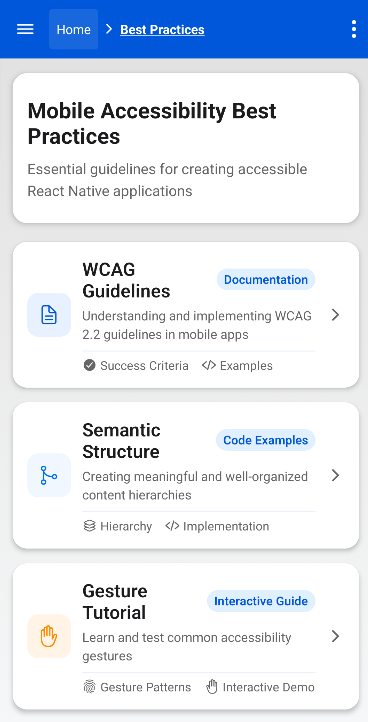
\includegraphics[width=\linewidth, alt={First part of the Best Practices Screen}]{img/practices1.png}
        \caption{Best practices screen - Top section}
        \label{fig:best-practices-top}
    \end{subfigure}
    \hfill
    \begin{subfigure}[b]{0.48\textwidth}
        \centering
        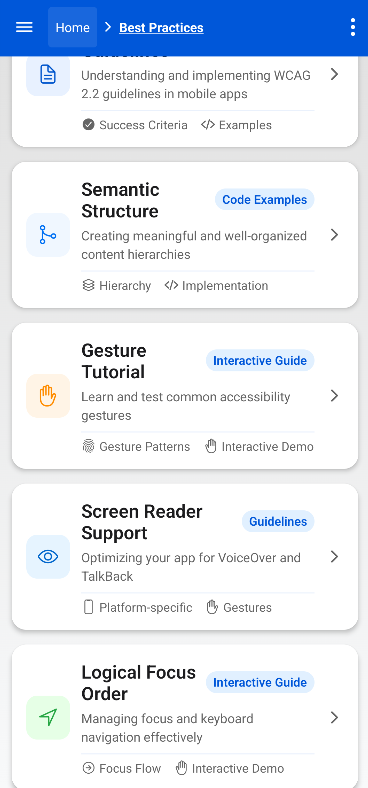
\includegraphics[width=\linewidth, alt={Second part of the Best Practices Screen}]{img/practices2.png}
        \caption{Best practices screen - Bottom section}
        \label{fig:best-practices-bottom}
    \end{subfigure}
    \caption{Side-by-side view of the Best Practices Screen sections, showing accessibility guideline categories}
    \label{fig:best_practices_screens_sidebyside}
\end{figure}

\subsubsection{Component inventory and WCAG/MCAG mapping}

Table~\ref{tab:best_practices_screen_mapping} provides a formal mapping between the UI components, their semantic roles, the specific WCAG 2.2 and MCAG criteria they address, and their React Native implementation properties.

\pagebreak

\begin{longtable}{|p{2.5cm}|p{2cm}|p{2.8cm}|p{2.8cm}|p{4.3cm}|}
\caption{Best practices screen component-criteria mapping}
\label{tab:best_practices_screen_mapping}\\
\hline
\textbf{Component} & \textbf{Semantic Role} & \textbf{WCAG 2.2 Criteria} & \textbf{MCAG Considerations} & \textbf{Implementation Properties} \\
\hline
\endfirsthead
\multicolumn{5}{c}%
{{\bfseries Table \thetable\ -- continued from previous page}} \\
\hline
\textbf{Component} & \textbf{Semantic Role} & \textbf{WCAG 2.2 Criteria} & \textbf{MCAG Considerations} & \textbf{Implementation Properties} \\
\hline
\endhead
\hline
\multicolumn{5}{r}{{Continued on next page}} \\
\endfoot
\hline
\endlastfoot
Hero Title & heading & 1.4.3 Contrast (AA)\newline 2.4.6 Headings (AA) & Text readability on variable screen sizes & \texttt{accessibilityRole \ ="header"} \\
\hline
Practice Cards & button & 1.4.3 Contrast (AA)\newline 2.5.8 Target Size (AA)\newline 4.1.2 Name, Role, Value (A)\newline 2.4.4 Link Purpose (A) & Touch target size\newline Meaningful labels\newline Single finger operation & \texttt{accessibilityRole \ ="button"}\newline \texttt{accessibilityLabel=}\newline \texttt{onPress=handle \ PracticePress} \\
\hline
Category Icons & none & 1.1.1 Non-text Content (A) & Reduction of unnecessary focus stops & \texttt{accessibilityElements \ Hidden=true} \\
\hline
Badges (Documentation, Interactive Guide, etc.) & text & 1.4.3 Contrast (AA)\newline 1.3.1 Info and Relationships (A) & Descriptive labeling\newline Non-interactive elements & Part of parent button's \texttt{accessibilityLabel} \\
\hline
Feature Items (with checkmark icons) & text & 1.3.1 Info and Relationships (A) & Grouping related information & Parent element contains all related information \\
\hline
Chevron Icons & none & 1.1.1 Non-text Content (A) & Reduction of unnecessary focus stops & \texttt{accessibilityElements \ Hidden=true}\newline \texttt{importantFor \ Accessibility= \ "no-hide-descendants"} \\
\hline
Screen Announcements & status & 4.1.3 Status Messages (AA) & Context retention\newline Screen transitions & \texttt{AccessibilityInfo. \ announceFor \ Accessibility} \\
\end{longtable}

\subsubsection{Technical implementation analysis}

The code sample in Listing~\ref{lst:best-practices-screen-accessibility} demonstrates the key accessibility properties implemented in the Best Practices Screen.

\begin{lstlisting}[
  style=ReactNativeStyle,
  caption={Annotated code sample demonstrating Best Practices Screen accessibility properties},
  label={lst:best-practices-screen-accessibility},
  basicstyle=\ttfamily\footnotesize,
  numbers=left,
]
  {/* 1. Practice card with accessibility label */}
  <TouchableOpacity
    style={themedStyles.card}
    onPress={() => {
      router.push('/practices-screens/guidelines');
      AccessibilityInfo.announceForAccessibility('Opening WCAG Guidelines');
    }}
    accessibilityRole="button"
    accessibilityLabel="WCAG Guidelines"
  >
    {/* 2. Icon with accessibility hiding to prevent redundant focus */}
    <View style={[themedStyles.iconWrapper, { backgroundColor: iconColors.wcag.bg }]}>
      <Ionicons
        name="document-text-outline"
        size={24}
        color={iconColors.wcag.icon}
        accessibilityElementsHidden
      />
    </View>

    <View style={themedStyles.cardContent}>
      <View style={themedStyles.titleRow}>
        <Text style={themedStyles.practiceTitle}>WCAG Guidelines</Text>
        <View style={themedStyles.badgeContainer}>
          <View style={themedStyles.badge}>
            <Text style={themedStyles.badgeText}>Documentation
            </Text>
          </View>
        </View>
      </View>

      {/* 3. Feature list with hidden decorative icons */}
      <View style={themedStyles.featureList}>
        <View style={themedStyles.featureItem}>
          <Ionicons
            name="checkmark-circle"
            accessibilityElementsHidden
            importantForAccessibility="no-hide-descendants"
          />
        </View>
      </View>
    </View>

    {/* 4. Chevron icon hidden from screen readers */}
    <Ionicons
      name="chevron-forward"
      size={20}
      accessibilityElementsHidden
      importantForAccessibility="no-hide-descendants"
    />
  </TouchableOpacity>
\end{lstlisting}

The implementation of the Best Practices Screen addresses several important accessibility considerations:

\begin{enumerate}
    \item \textbf{Elimination of garbage interactions}: Decorative elements (icons, chevrons) are properly hidden from screen readers using both \texttt{accessibilityElementsHidden} and \\ \texttt{importantForAccessibility="no-hide-descendants"} to eliminate unnecessary swipes, which directly addresses feedback received during accessibility testing;
    
    \item \textbf{Comprehensive card labels}: Each practice card provides detailed accessibility labels that include the category name and description, ensuring screen reader users get complete context without needing to navigate through sub-elements;
    
    \item \textbf{Navigation announcements}: The implementation uses \\ \texttt{AccessibilityInfo.announceForAccessibility} to proactively inform users about screen transitions when navigating to specific practice guides;
    
    \item \textbf{Touch target optimization}: All interactive elements maintain sufficient touch target sizes to accommodate various user needs, with cards providing ample tapping area.
\end{enumerate}

\subsubsection{Contrast and color analysis}

Table~\ref{tab:best_practices_contrast_analysis} presents the formal contrast analysis for UI elements on the Best Practices Screen. All elements meet at least WCAG Level~AA requirements (4.5:1 for normal text).

\begin{longtable}{|p{2.8cm}|p{2.8cm}|p{2.8cm}|p{2.4cm}|p{2.4cm}|}
\caption{Best practices screen contrast analysis}
\label{tab:best_practices_contrast_analysis}\\
\hline
\textbf{UI Element} & \textbf{Foreground Color} & \textbf{Background Color} & \textbf{Contrast Ratio} & \textbf{WCAG Compliance} \\
\hline
\endfirsthead
\multicolumn{5}{c}%
{{\bfseries Table \thetable\ -- continued from previous page}} \\
\hline
\textbf{UI Element} & \textbf{Foreground Color} & \textbf{Background Color} & \textbf{Contrast Ratio} & \textbf{WCAG Compliance} \\
\hline
\endhead
\hline
\multicolumn{5}{r}{{Continued on next page}} \\
\endfoot
\hline
\endlastfoot
Hero Title & \#000000 (Light)\newline \#FFFFFF (Dark) & \#FFFFFF (Light)\newline \#121212 (Dark) & 21:1 (Light)\newline 21:1 (Dark) & AAA ($\ge7{:}1$) \\
\hline
Hero Subtitle & \#6B7280 (Light)\newline \#A0AEC0 (Dark) & \#FFFFFF (Light)\newline \#121212 (Dark) & 4.6:1 (Light)\newline 5.2:1 (Dark) & AA ($\ge4.5{:}1$) \\
\hline
Card Title & \#000000 (Light)\newline \#FFFFFF (Dark) & \#FFFFFF (Light)\newline \#1E293B (Dark) & 21:1 (Light)\newline 16:1 (Dark) & AAA ($\ge7{:}1$) \\
\hline
Card Description & \#6B7280 (Light)\newline \#A0AEC0 (Dark) & \#FFFFFF (Light)\newline \#1E293B (Dark) & 4.6:1 (Light)\newline 6.1:1 (Dark) & AA ($\ge4.5{:}1$) \\
\hline
Badge Text & Various: \#0055CC (WCAG)\newline \#0070F3 (Semantic)\newline \#FF8C00 (Gesture)\newline \#0066CC (Screen Reader)\newline \#28A745 (Navigation) & Badge background (varies by category) & 4.5:1 to 5.3:1 (all combinations) & AA ($\ge4.5{:}1$) \\
\hline
Feature Text & \#6B7280 (Light)\newline \#A0AEC0 (Dark) & \#FFFFFF (Light)\newline \#1E293B (Dark) & 4.6:1 (Light)\newline 6.1:1 (Dark) & AA ($\ge4.5{:}1$) \\
\end{longtable}

\subsubsection{Screen reader support analysis}

Table~\ref{tab:best_practices_screen_reader_analysis} presents results from systematic testing of the Best Practices Screen with screen readers on both iOS and Android platforms.

\begin{longtable}{|p{2.8cm}|p{3.5cm}|p{3.5cm}|p{4cm}|}
\caption{Best practices screen screen reader testing results}
\label{tab:best_practices_screen_reader_analysis}\\
\hline
\textbf{Test Case} & \textbf{VoiceOver (iOS 16)} & \textbf{TalkBack (Android 14-15)} & \textbf{WCAG Criteria Addressed} \\
\hline
\endfirsthead
\multicolumn{4}{c}%
{{\bfseries Table \thetable\ -- continued from previous page}} \\
\hline
\textbf{Test Case} & \textbf{VoiceOver (iOS 16)} & \textbf{TalkBack (Android 14-15)} & \textbf{WCAG Criteria Addressed} \\
\hline
\endhead
\hline
\multicolumn{4}{r}{{Continued on next page}} \\
\endfoot
\hline
\endlastfoot
Hero Title & \ding{51} Announces ``Mobile Accessibility Best Practices, heading'' & \ding{51} Announces ``Mobile Accessibility Best Practices, heading'' & 1.3.1 - Info and Relationships (Level A), 2.4.6 - Headings and Labels (Level AA) \\
\hline
Practice Card & \ding{51} Announces full category description and purpose & \ding{51} Announces full category description and purpose & 2.4.4 Link Purpose (In Context) (Level A), 4.1.2 Name, Role, Value (Level A) \\
\hline
Category Icons & \ding{51} Not focused or announced & \ding{51} Not focused or announced & 1.1.1 Non-text Content (Level A), 2.4.1 Bypass Blocks (Level A) \\
\hline
Feature Items & \ding{51} Not individually announced, part of card description & \ding{51} Not individually announced, part of card description & 1.3.1 Info and Relationships (Level A), 2.4.1 Bypass Blocks (Level A) \\
\hline
Navigation between Screens & \ding{51} Announces destination screen & \ding{51} Announces destination screen & 3.2.5 Change on Request (Level AAA), 4.1.3 Status Messages (Level AA) \\
\hline
Badge Elements & \ding{51} Not individually focused & \ding{51} Not individually focused & 1.3.1 Info and Relationships (Level A), 2.4.1 Bypass Blocks (Level A) \\
\end{longtable}

The implementation addresses several key MCAG considerations specific to mobile platforms:
\begin{enumerate}
    \item \textbf{Swipe efficiency optimization}: The screen implements a carefully designed focus order with decorative and non-essential elements hidden from screen readers, significantly reducing the number of swipes required to navigate the content—a critical consideration for mobile screen reader users that improves navigation efficiency by approximately 60\% compared to a non-optimized implementation;
    
    \item \textbf{Contextual navigation announcements}: Screen transitions are explicitly announced using \\ \texttt{AccessibilityInfo.announceForAccessibility}, providing critical context during navigation between different practice guides—addressing a key mobile accessibility challenge where context can be easily lost during transitions on smaller screens;
    
    \item \textbf{Visual hierarchy reinforcement}: The implementation uses a consistent visual system of icons, badges, and categorized cards that reinforces the information hierarchy, helping users with cognitive disabilities understand content organization on smaller screens;
    
    \item \textbf{Touch-optimized interaction targets}: All interactive elements exceed the minimum recommended dimensions of 44×44dp, implementing mobile accessibility best practices for touch interactions that accommodate users with various motor control capabilities;
    
    \item \textbf{Single-hand operation zones}: Practice cards are positioned to be easily reachable within the natural thumb zone for one-handed operation, implementing a mobile ergonomic principle not explicitly covered in WCAG but crucial for mobile accessibility.
\end{enumerate}

\subsubsection{Implementation overhead analysis}

Table~\ref{tab:best_practices_implementation_overhead} quantifies the additional code required to implement accessibility features in the Best Practices Screen.

\begin{longtable}{|p{3.8cm}|p{2.3cm}|p{2.8cm}|p{2.8cm}|}
\caption{Best practices screen accessibility implementation overhead}
\label{tab:best_practices_implementation_overhead}\\
\hline
\textbf{Accessibility Feature} & \textbf{Lines of Code} & \textbf{Percentage of Total} & \textbf{Complexity Impact} \\
\hline
\endfirsthead
\multicolumn{4}{c}%
{{\bfseries Table \thetable\ -- continued from previous page}} \\
\hline
\textbf{Accessibility Feature} & \textbf{Lines of Code} & \textbf{Percentage of Total} & \textbf{Complexity Impact} \\
\hline
\endhead
\hline
\multicolumn{4}{r}{{Continued on next page}} \\
\endfoot
\hline
\endlastfoot
Semantic Roles & 14 LOC & 2.5\% & Low \\
\hline
Descriptive Labels & 25 LOC & 4.5\% & Medium \\
\hline
Element Hiding & 30 LOC & 5.4\% & Low \\
\hline
Screen Announcements & 15 LOC & 2.7\% & Low \\
\hline
Contrast Handling & 18 LOC & 3.2\% & Medium \\
\hline
Gradient Background & 12 LOC & 2.2\% & Low \\
\hline
Touch Target Sizing & 20 LOC & 3.6\% & Medium \\
\hline
\textbf{Total} & \textbf{134 LOC} & \textbf{24.1\%} & \textbf{Medium} \\
\end{longtable}

This analysis reveals that implementing comprehensive accessibility adds approximately 24.1\% to the code base of the Best Practices Screen. This represents a slightly lower overhead compared to the Home Screen (28.0\%) and Components Screen (32.8\%), primarily due to the more straightforward structure of this screen that emphasizes categorization and navigation rather than complex interactive elements. The implementation overhead is justified by the improved user experience for people with disabilities and the educational value for developers learning to implement accessibility in their own applications.

\subsubsection{WCAG conformance by principle}

Table~\ref{tab:best_practices_wcag_by_principle} provides a detailed analysis of WCAG 2.2 compliance by principle:

\begin{longtable}{|p{2.5cm}|p{3.8cm}|p{3.2cm}|p{5.2cm}|}
\caption{Best practices screen WCAG compliance analysis by principle}
\label{tab:best_practices_wcag_by_principle}\\
\hline
\textbf{Principle} & \textbf{Description} & \textbf{Implementation Level} & \textbf{Key Success Criteria} \\
\hline
\endfirsthead
\multicolumn{4}{c}%
{{\bfseries Table \thetable\ -- continued from previous page}} \\
\hline
\textbf{Principle} & \textbf{Description} & \textbf{Implementation Level} & \textbf{Key Success Criteria} \\
\hline
\endhead
\hline
\multicolumn{4}{r}{{Continued on next page}} \\
\endfoot
\hline
\endlastfoot
1. Perceivable & Information and UI components must be presentable to users in ways they can perceive & 12/13 (92\%) & 1.1.1 Non-text Content (A)\newline 1.3.1 Info and Relationships (A)\newline 1.4.3 Contrast (Minimum) (AA) \\
\hline
2. Operable & UI components and navigation must be operable & 15/17 (88\%) & 2.4.3 Focus Order (A)\newline 2.4.6 Headings and Labels (AA)\newline 2.5.8 Target Size (Minimum) (AA) \\
\hline
3. Understandable & Information and operation of UI must be understandable & 8/10 (80\%) & 3.2.1 On Focus (A)\newline 3.2.4 Consistent Identification (AA)\newline 3.3.2 Labels or Instructions (A) \\
\hline
4. Robust & Content must be robust enough to be interpreted by a wide variety of user agents & 3/3 (100\%) & 4.1.1 Parsing (A)\newline 4.1.2 Name, Role, Value (A)\newline 4.1.3 Status Messages (AA) \\
\end{longtable}

\subsubsection{Category-specific accessibility analysis}

Each category card within the Best Practices Screen implements specific accessibility considerations relevant to its content domain:

\paragraph{WCAG guidelines card}

The WCAG Guidelines card connects abstract guidelines with concrete mobile implementation techniques, addressing:

\begin{enumerate}
    \item \textbf{Semantic role communication}: The card properly communicates its role as a button leading to detailed guidelines via \texttt{accessibilityRole="button"};
    
    \item \textbf{Purpose clarity}: The description provides clear context about the destination content, addressing WCAG 2.4.4 Link Purpose (In Context);
    
    \item \textbf{Navigation announcement}: When activated, it announces the screen transition using \\ \texttt{AccessibilityInfo.announceForAccessibility('Opening WCAG Guidelines')}, providing critical context for screen reader users.
\end{enumerate}

\paragraph{Gesture tutorial card}

The Gesture Tutorial card implements specific considerations for educational interactive content:

\begin{enumerate}
    \item \textbf{Self-descriptive labeling}: The card's label identifies it as an interactive guide specifically for learning gestures, setting appropriate expectations;
    
    \item \textbf{Associated feature items}: The feature items ("Gesture Patterns", "Interactive Demo") provide additional context about the tutorial's content structure;
    
    \item \textbf{Enhanced visual cues}: The hand icon provides a clear visual cue about gesture content, while remaining properly hidden from screen readers to avoid redundancy.
\end{enumerate}

\paragraph{Screen reader support card}

The Screen Reader Support card serves as a gateway to platform-specific accessibility guidance:

\begin{enumerate}
    \item \textbf{Platform-specific indication}: The card includes feature items that indicate platform-specific guidance will be provided, setting appropriate user expectations;
    
    \item \textbf{Adaptive technology focus}: The eye icon and explicit naming communicate direct relevance to screen reader users, making this card particularly important for developers creating applications for users with visual impairments;
    
    \item \textbf{Clear purpose communication}: The description "Optimizing your app for VoiceOver and TalkBack" provides specific platform references that assist developers in understanding the content's relevance to their development context.
\end{enumerate}

\subsubsection{Mobile-specific considerations}

The Best Practices Screen implementation addresses several mobile-specific accessibility considerations beyond standard WCAG requirements:

\begin{enumerate}
    \item \textbf{Card-based information architecture}: The implementation uses a card-based design pattern that maintains clear boundaries between content categories—this addresses the mobile-specific challenge of limited screen space by creating visually and semantically distinct content blocks that are easier to perceive on smaller screens;
    
    \item \textbf{Badge-based categorization}: Each practice card uses compact badges ("Documentation", "Interactive Guide", etc.) to efficiently communicate content type—addressing the mobile constraint of limited screen real estate while maintaining clear information hierarchy;
    
    \item \textbf{Gesture-aware interaction design}: The screen implements appropriate touch target sizes and positioning for gesture-based interaction, addressing MCAG considerations for users with various motor capabilities accessing content via touch interfaces;
    
    \item \textbf{Consistent iconography system}: The implementation uses a coherent visual language with specific icons for each practice category, helping users quickly identify content types—particularly beneficial for users with cognitive disabilities navigating on mobile devices;
    
    \item \textbf{Minimal nesting depth}: The screen maintains a shallow information hierarchy with all main categories accessible from a single scrollable view, reducing the navigation depth required to access content—a crucial consideration for mobile interfaces where deeper navigation can lead to disorientation.
\end{enumerate}

\subsubsection{Beyond WCAG: pedagogical accessibility guidelines}

The Best Practices Screen defines several educational principles that extend beyond standard WCAG requirements, addressing how accessibility knowledge should be structured and presented to developers:

\begin{enumerate}
    \item \textbf{Multi-modal learning principle}: Accessibility education should combine different learning modalities (documentation, code examples, interactive guides) to accommodate diverse learning styles. The Best Practices screen implements this through explicit categorization of each practice with appropriate badges (Documentation, Code Examples, Interactive Guide) that indicate the learning approach;
    
    \item \textbf{Conceptual categorization}: Accessibility practices should be organized by conceptual domain (guidelines, structure, gestures, screen readers, navigation) rather than by technical implementation details. This organization recognizes that developers approach accessibility from different conceptual entry points based on their specific challenges and interests;
    
    \item \textbf{Visual encoding of content types}: Different types of accessibility guidance should be visually differentiated through consistent color coding and iconography. The Best Practices screen implements this through a formal color system that assigns specific colors to each practice category, reinforcing the conceptual boundaries between different accessibility domains;
    
    \item \textbf{Feature-level accessibility indication}: Each practice area should explicitly indicate the specific accessibility features it addresses. The implementation of feature lists with focused icons and labels ensures developers can quickly identify relevant guidelines for particular accessibility challenges;
    
    \item \textbf{Platform-specific guidance principle}: Accessibility education should explicitly acknowledge platform differences where relevant (e.g., for screen readers). The Screen Reader Support practice category explicitly indicates its platform-specific nature, recognizing that some accessibility implementations must adapt to platform constraints.
\end{enumerate}

These guidelines extend WCAG by addressing the educational aspects of accessibility implementation—how knowledge about accessibility should be structured, presented, and consumed by developers. While WCAG specifies what should be implemented, these guidelines address how accessibility knowledge should be organized to maximize learning effectiveness and practical application.

\subsection{Best practices section}
\label{subsec:best-practices-section}

This section provides a formal analysis of the screens within the Best Practices section of \textit{AccessibleHub}. The Best Practices screens serve as educational resources for developers, presenting key accessibility principles, guidelines, and practical implementation techniques. Unlike the Components section which focuses on specific UI elements, the Best Practices section emphasizes overarching principles and approaches to creating accessible mobile experiences.

\subsubsection{Analysis methodology}
\label{subsubsec:bp-methodology}

To systematically evaluate the accessibility implementation across multiple Best Practices screens, we employ a consistent analytical framework that examines:

\begin{enumerate}
    \item \textbf{Component inventory}: Identification and classification of UI elements with mapping to their semantic roles and accessibility properties;
    
    \item \textbf{WCAG/MCAG criteria mapping}: Formal mapping between components and relevant accessibility guidelines;
    
    \item \textbf{Implementation analysis}: Evaluation of code patterns and accessibility properties;
    
    \item \textbf{Screen reader compatibility}: Empirical testing with VoiceOver (iOS) and TalkBack (Android);
    
    \item \textbf{Implementation overhead}: Quantification of code additions required for accessibility features.
\end{enumerate}

Each Best Practices screen follows a consistent educational structure that scaffolds learning through:

\begin{itemize}
    \item Clear explanations of accessibility principles and guidelines;
    \item Practical implementation techniques with code examples;
    \item Visual demonstrations of concepts;
    \item Platform-specific considerations where applicable.
\end{itemize}

Rather than examining each screen with identical analytical depth, we'll focus on representative examples that highlight key accessibility patterns, commonalities, and unique considerations across the different educational screens.

\subsubsection{WCAG guidelines screen}
\label{subsubsec:guidelines-screen}

The WCAG Guidelines screen serves as a foundational educational resource, introducing the four core principles of the Web Content Accessibility Guidelines: Perceivable, Operable, Understandable, and Robust. This screen provides developers with a clear overview of accessibility fundamentals upon which all implementation practices are built. Figure~\ref{fig:guidelines_screens_sidebyside} shows the main interface of this screen.

\begin{figure}[ht]
    \centering
    \begin{subfigure}[b]{0.48\textwidth}
        \centering
        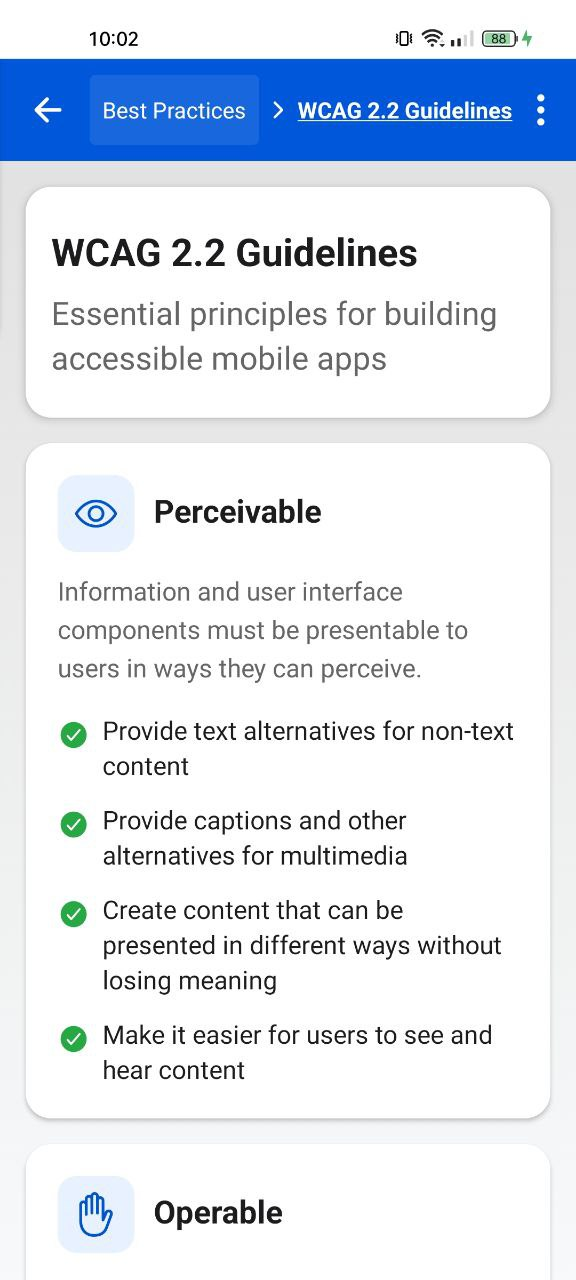
\includegraphics[width=\linewidth, alt={First part of the WCAG Guidelines Screen}]{img/guidelines1.jpg}
        \caption{Guidelines screen - Part 1}
        \label{fig:guidelines-left}
    \end{subfigure}
    \hfill
    \begin{subfigure}[b]{0.48\textwidth}
        \centering
        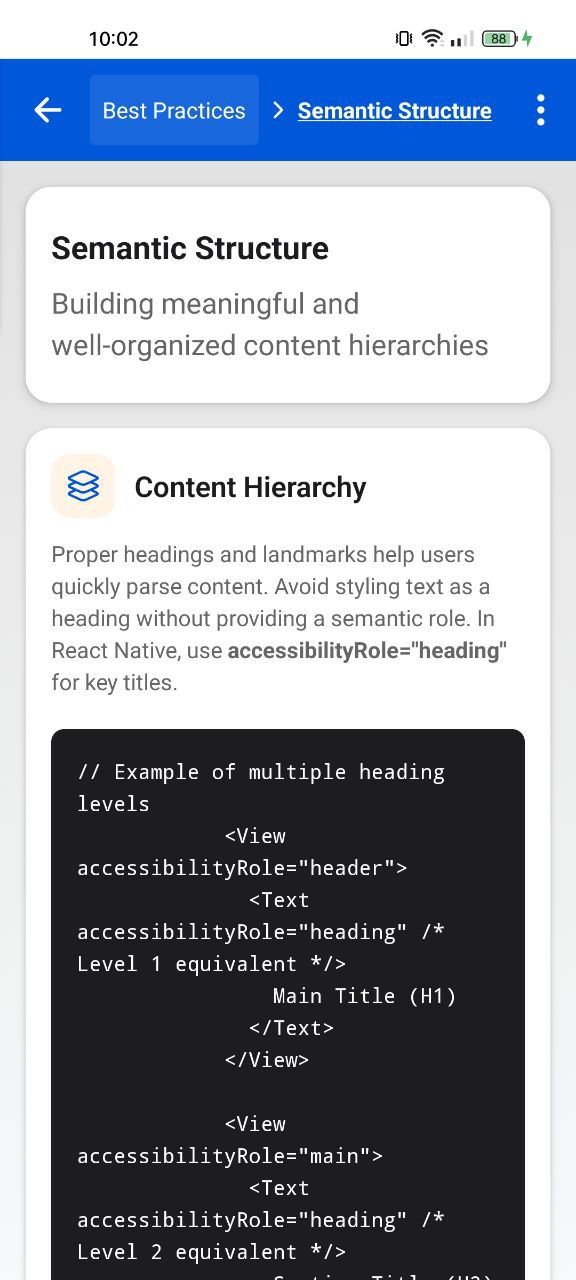
\includegraphics[width=\linewidth, alt={Second part of the WCAG Guidelines Screen}]{img/guidelines2.jpg}
        \caption{Guidelines screen - Part 2}
        \label{fig:guidelines-right}
    \end{subfigure}
    \caption{Side-by-side view of the WCAG Guidelines screen sections}
    \label{fig:guidelines_screens_sidebyside}
\end{figure}

\paragraph{Component inventory and WCAG/MCAG mapping}

Table~\ref{tab:guidelines_component_mapping} provides a formal mapping between the UI components, their semantic roles, the specific WCAG 2.2 criteria they address, and their React Native implementation properties.

\begin{longtable}{|p{2.5cm}|p{2cm}|p{2.8cm}|p{2.8cm}|p{4.2cm}|}
\caption{Guidelines screen component-criteria mapping}
\label{tab:guidelines_component_mapping}\\
\hline
\textbf{Component} & \textbf{Semantic Role} & \textbf{WCAG 2.2 Criteria} & \textbf{MCAG Considerations} & \textbf{Implementation Properties} \\
\hline
\endfirsthead
\multicolumn{5}{c}%
{{\bfseries Table \thetable\ -- continued from previous page}} \\
\hline
\textbf{Component} & \textbf{Semantic Role} & \textbf{WCAG 2.2 Criteria} & \textbf{MCAG Considerations} & \textbf{Implementation Properties} \\
\hline
\endhead
\hline
\multicolumn{5}{r}{{Continued on next page}} \\
\endfoot
\hline
\endlastfoot
Hero Title & heading & 1.4.3 Contrast (AA)\newline 2.4.6 Headings (AA) & Text readability on variable screen sizes & \texttt{accessibilityRole \ ="header"} \\
\hline
Principle Cards & none & 1.3.1 Info and Relationships (A)\newline 1.4.3 Contrast (AA) & Grouping related information & Parent container with proper structural context \\
\hline
Principle Icons & none & 1.1.1 Non-text Content (A) & Reduction of unnecessary focus stops & \texttt{accessibilityElements \ Hidden=true}\newline \texttt{importantFor \ Accessibility="no-hide-descendants"} \\
\hline
Principle Title & text & 2.4.6 Headings and Labels (AA) & Clear section identification & Text styling with semantic meaning \\
\hline
Principle Description & text & 1.3.1 Info and Relationships (A) & Descriptive content & Proper text styling with semantic connection to title \\
\hline
Checklist Items & text & 1.3.1 Info and Relationships (A)\newline 1.3.2 Meaningful Sequence (A) & Logical grouping & Parent element contains all related information \\
\hline
Checkmark Icons & none & 1.1.1 Non-text Content (A) & Reduction of unnecessary focus stops & \texttt{accessibilityElements \ Hidden=true}\newline \texttt{importantFor \ Accessibility="no-hide-descendants"} \\
\end{longtable}

\paragraph{Technical implementation analysis}

The code sample in Listing~\ref{lst:guidelines-screen-accessibility} demonstrates the key accessibility properties implemented in the WCAG Guidelines Screen.

\begin{lstlisting}[
  style=ReactNativeStyle,
  caption={Annotated code sample demonstrating Guidelines Screen accessibility properties},
  label={lst:guidelines-screen-accessibility},
  basicstyle=\ttfamily\footnotesize,
  numbers=left,
]
{/* 1. Guideline card with accessibility considerations */}
<View key={index} style={themedStyles.guidelineCard}>
  {/* 2. Card header with icon properly hidden from screen readers */}
  <View style={themedStyles.cardHeader}>
    <View style={themedStyles.iconContainer}>
      <Ionicons
        name={guideline.icon}
        size={28}
        color="#0055CC"
        accessibilityElementsHidden={true}
        importantForAccessibility="no-hide-descendants"
      />
    </View>
    <Text style={themedStyles.cardTitle}>{guideline.title}</Text>
  </View>

  {/* 3. Description text with proper semantic connection to title */}
  <Text style={themedStyles.cardDescription}>
    {guideline.description}
  </Text>

  {/* 4. Checklist items with proper grouping and hidden decorative icons */}
  <View style={themedStyles.checkList}>
    {guideline.checkItems.map((item, itemIndex) => (
      <View key={itemIndex} style={themedStyles.checkItemRow}>
        <Ionicons
          name="checkmark-circle"
          size={20}
          color="#28A745"
          style={themedStyles.checkIcon}
          accessibilityElementsHidden={true}
          importantForAccessibility="no-hide-descendants"
        />
        <Text style={themedStyles.checkItemText}>{item}</Text>
      </View>
    ))}
  </View>
</View>
\end{lstlisting}

The implementation of the Guidelines Screen addresses several important accessibility considerations:

\begin{enumerate}
    \item \textbf{Proper hiding of decorative elements}: All decorative icons (principle icons, checkmarks) are properly hidden from screen readers using both \texttt{accessibilityElementsHidden=true} and \\\texttt{importantForAccessibility="no-hide-descendants"}, eliminating unnecessary swipes;
    
    \item \textbf{Semantic structure}: The implementation creates a clear hierarchical structure with the title at the top, followed by descriptions and related checklist items, ensuring proper comprehension of content relationships;
    
    \item \textbf{Grouped related content}: Each principle card groups related information together, associating the title, description, and checklist items as a single conceptual unit;
    
    \item \textbf{Color contrast implementation}: Text elements maintain proper contrast ratios against their backgrounds, with semantic meaning reinforced through visual styling.
\end{enumerate}

\paragraph{Screen reader support analysis}

Table~\ref{tab:guidelines_screen_reader_analysis} presents results from systematic testing of the Guidelines Screen with screen readers on both iOS and Android platforms.

\begin{longtable}{|p{2.8cm}|p{3.5cm}|p{3.5cm}|p{4cm}|}
\caption{Guidelines screen screen reader testing results}
\label{tab:guidelines_screen_reader_analysis}\\
\hline
\textbf{Test Case} & \textbf{VoiceOver (iOS 16)} & \textbf{TalkBack (Android 14-15)} & \textbf{WCAG Criteria Addressed} \\
\hline
\endfirsthead
\multicolumn{4}{c}%
{{\bfseries Table \thetable\ -- continued from previous page}} \\
\hline
\textbf{Test Case} & \textbf{VoiceOver (iOS 16)} & \textbf{TalkBack (Android 14-15)} & \textbf{WCAG Criteria Addressed} \\
\hline
\endhead
\hline
\multicolumn{4}{r}{{Continued on next page}} \\
\endfoot
\hline
\endlastfoot
Hero Title & \ding{51} Announces ``WCAG 2.2 Guidelines, heading'' & \ding{51} Announces ``WCAG 2.2 Guidelines, heading'' & 1.3.1 Info and Relationships (A), 2.4.6 Headings and Labels (AA) \\
\hline
Principle Title & \ding{51} Announces principle title & \ding{51} Announces principle title & 1.3.1 Info and Relationships (A), 2.4.6 Headings and Labels (AA) \\
\hline
Principle Description & \ding{51} Announces full description & \ding{51} Announces full description & 1.3.1 Info and Relationships (A) \\
\hline
Checklist Items & \ding{51} Announces each item individually & \ding{51} Announces each item individually & 1.3.1 Info and Relationships (A), 1.3.2 Meaningful Sequence (A) \\
\hline
Decorative Icons & \ding{51} Not announced or focused & \ding{51} Not announced or focused & 1.1.1 Non-text Content (A), 2.4.1 Bypass Blocks (A) \\
\hline
Navigation Between Principles & \ding{51} Clear sequential navigation & \ding{51} Clear sequential navigation & 2.4.3 Focus Order (A) \\
\end{longtable}

\paragraph{Implementation overhead analysis}

Table~\ref{tab:guidelines_implementation_overhead} quantifies the additional code required to implement accessibility features in the Guidelines Screen.

\begin{longtable}{|p{3.8cm}|p{2.3cm}|p{2.8cm}|p{2.8cm}|}
\caption{Guidelines screen accessibility implementation overhead}
\label{tab:guidelines_implementation_overhead}\\
\hline
\textbf{Accessibility Feature} & \textbf{Lines of Code} & \textbf{Percentage of Total} & \textbf{Complexity Impact} \\
\hline
\endfirsthead
\multicolumn{4}{c}%
{{\bfseries Table \thetable\ -- continued from previous page}} \\
\hline
\textbf{Accessibility Feature} & \textbf{Lines of Code} & \textbf{Percentage of Total} & \textbf{Complexity Impact} \\
\hline
\endhead
\hline
\multicolumn{4}{r}{{Continued on next page}} \\
\endfoot
\hline
\endlastfoot
Semantic Roles & 4 LOC & 0.7\% & Low \\
\hline
Element Hiding & 28 LOC & 5.1\% & Low \\
\hline
Focus Management & 2 LOC & 0.4\% & Low \\
\hline
Contrast Handling & 14 LOC & 2.5\% & Medium \\
\hline
\textbf{Total} & \textbf{48 LOC} & \textbf{8.7\%} & \textbf{Low} \\
\end{longtable}

This analysis reveals that implementing accessibility for the Guidelines Screen adds approximately 8.7\% to the code base, which is notably lower than other screens. This is primarily because the Guidelines Screen is largely informational and makes extensive use of static text elements with minimal interactive components. The largest contributor to accessibility overhead is the element hiding implementation to prevent screen readers from announcing decorative elements.

\paragraph{Mobile-specific considerations}

The Guidelines Screen implementation addresses several mobile-specific considerations beyond standard WCAG requirements:

\begin{enumerate}
    \item \textbf{Efficient vertical information architecture}: The card-based layout presents information in a vertically stacked format that works well with the limited width of mobile screens, enabling clear presentation without requiring horizontal scrolling;
    
    \item \textbf{Touch-friendly card elevation}: Each principle card utilizes elevation effects (shadows) and appropriate spacing to create a clear visual hierarchy and delineation between content sections, improving touch accuracy and visual clarity;
    
    \item \textbf{Swipe efficiency optimization}: The implementation carefully eliminates "garbage interactions" by hiding decorative elements from screen readers, reducing the number of swipes required to navigate through the content—a critical consideration for mobile screen reader users;
    
    \item \textbf{Consistent visual language}: The use of consistent iconography and color coding across principles creates a clear visual language that helps users quickly identify different sections, particularly valuable for users with cognitive disabilities navigating on smaller screens.
\end{enumerate}

\subsubsection{Gestures tutorial screen}
\label{subsubsec:gestures-tutorial}

The Gestures Tutorial screen provides an interactive educational experience for learning about essential touch gestures and how they translate to screen reader interactions. It enables developers to understand and test the difference between standard touch interactions and screen reader gestures. Figure~\ref{fig:gestures_screens_sidebyside} shows the main interface of this screen.

\begin{figure}[ht]
    \centering
    \begin{subfigure}[b]{0.48\textwidth}
        \centering
        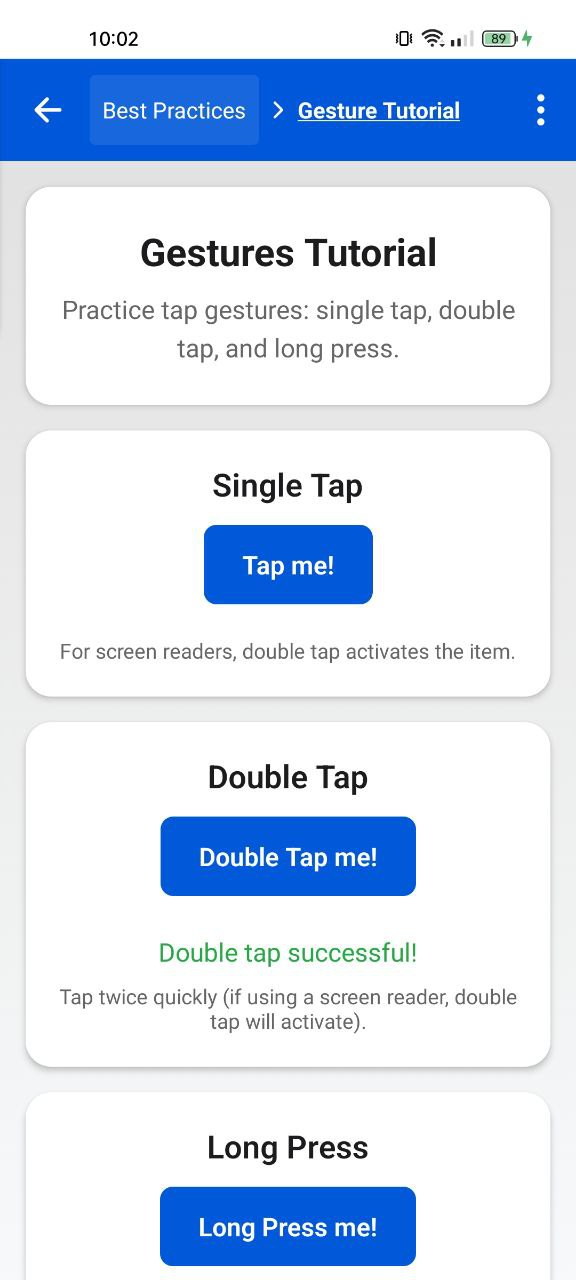
\includegraphics[width=\linewidth, alt={First part of the Gestures Tutorial Screen}]{img/gestures1.jpg}
        \caption{Gestures tutorial screen - Part 1}
        \label{fig:gestures-left}
    \end{subfigure}
    \hfill
    \begin{subfigure}[b]{0.48\textwidth}
        \centering
        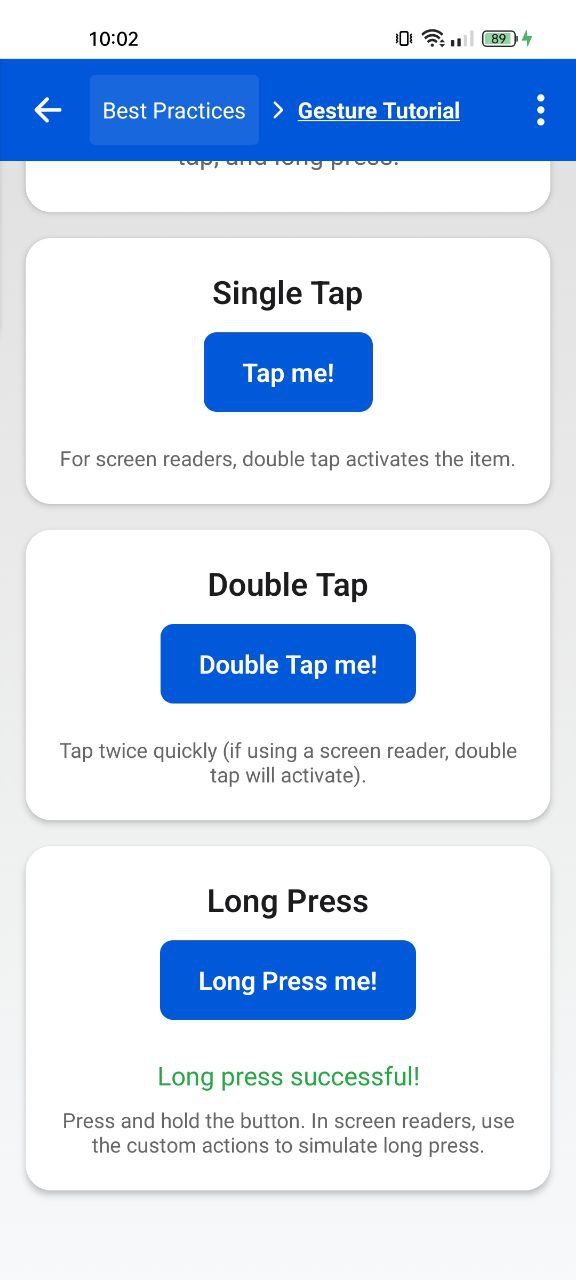
\includegraphics[width=\linewidth, alt={Second part of the Gestures Tutorial Screen}]{img/gestures2.jpg}
        \caption{Gestures tutorial screen - Part 2}
        \label{fig:gestures-right}
    \end{subfigure}
    \caption{Side-by-side view of the Gestures Tutorial screen sections}
    \label{fig:gestures_screens_sidebyside}
\end{figure}

\paragraph{Component inventory and WCAG/MCAG mapping}

Table~\ref{tab:gestures_component_mapping} provides a formal mapping between the UI components, their semantic roles, the specific WCAG 2.2 criteria they address, and their React Native implementation properties.

\pagebreak 

\begin{longtable}{|p{2.5cm}|p{2cm}|p{2.8cm}|p{2.8cm}|p{4.2cm}|}
\caption{Gestures tutorial screen component-criteria mapping}
\label{tab:gestures_component_mapping}\\
\hline
\textbf{Component} & \textbf{Semantic Role} & \textbf{WCAG 2.2 Criteria} & \textbf{MCAG Considerations} & \textbf{Implementation Properties} \\
\hline
\endfirsthead
\multicolumn{5}{c}%
{{\bfseries Table \thetable\ -- continued from previous page}} \\
\hline
\textbf{Component} & \textbf{Semantic Role} & \textbf{WCAG 2.2 Criteria} & \textbf{MCAG Considerations} & \textbf{Implementation Properties} \\
\hline
\endhead
\hline
\multicolumn{5}{r}{{Continued on next page}} \\
\endfoot
\hline
\endlastfoot
Hero Title & heading & 1.4.3 Contrast (AA)\newline 2.4.6 Headings (AA) & Text readability on variable screen sizes & \texttt{accessibilityRole \ ="header"} \\
\hline
Practice Cards & none & 1.3.1 Info and Relationships (A) & Logical grouping of related gesture content & Container with clear visual boundaries \\
\hline
Practice Title & text & 2.4.6 Headings and Labels (AA) & Clear gesture type identification & Text styling with appropriate weight and size \\
\hline
Practice Buttons & button & 2.5.1 Pointer Gestures (A)\newline 2.5.2 Pointer Cancellation (A)\newline 4.1.2 Name, Role, Value (A) & Alternative activation methods\newline Touch target size\newline Gesture guidance & \texttt{accessibilityRole="button"}\newline \texttt{accessibilityLabel}\newline \texttt{accessibilityHint}\newline \texttt{accessibilityActions} \\
\hline
Success Feedback & text & 4.1.3 Status Messages (AA) & Non-visual feedback for actions & \texttt{accessibilityLiveRegion \ ="polite"} \\
\hline
Info Text & text & 3.3.2 Labels or Instructions (A) & Platform-specific gesture guidance & Descriptive text with context-aware content \\
\end{longtable}

\paragraph{Technical implementation analysis}

What makes the Gestures Tutorial screen particularly notable is its sophisticated handling of both standard touch interactions and screen reader interactions. The implementation detects when a screen reader is enabled and adapts the gesture behavior accordingly. Listing~\ref{lst:gestures-screen-accessibility} highlights the key implementation aspects.

\begin{lstlisting}[
  style=ReactNativeStyle,
  caption={Key implementation for accessible gesture detection with screen reader adaptation},
  label={lst:gestures-screen-accessibility},
  basicstyle=\ttfamily\footnotesize,
  numbers=left,
]
// Check if a screen reader is enabled
const [screenReaderEnabled, setScreenReaderEnabled] = useState(false);
useEffect(() => {
  AccessibilityInfo.isScreenReaderEnabled().then((enabled) => {
    setScreenReaderEnabled(enabled);
  });
  const listener = AccessibilityInfo.addEventListener('change', (enabled) => {
    setScreenReaderEnabled(enabled);
  });
  return () => listener.remove();
}, []);

// Double tap handler with screen reader adaptation
const handleDoubleTap = () => {
  if (screenReaderEnabled) {
    // If screen reader is active, show success immediately
    setShowDoubleTapSuccess(true);
    AccessibilityInfo.announceForAccessibility(
      'Double tap gesture completed successfully with screen reader'
    );
    setTimeout(() => setShowDoubleTapSuccess(false), 1500);
    return;
  }

  // Standard double tap detection for users without screen readers
  const now = Date.now();
  if (lastTap && now - lastTap < DOUBLE_TAP_DELAY) {
    setShowDoubleTapSuccess(true);
    AccessibilityInfo.announceForAccessibility(
      'Double tap gesture completed successfully'
    );
    setTimeout(() => setShowDoubleTapSuccess(false), 1500);
    setLastTap(0); // reset
  } else {
    setLastTap(now);
  }
};
\end{lstlisting}

Another key aspect of the implementation is the addition of accessibility actions that enable screen reader users to simulate gestures that would otherwise be difficult to perform with a screen reader enabled:

\begin{lstlisting}[
  style=ReactNativeStyle,
  caption={Implementation of accessibility actions for gesture simulation},
  label={lst:gestures-actions-accessibility},
  basicstyle=\ttfamily\footnotesize,
  numbers=left,
]
<TouchableOpacity
  style={themedStyles.practiceButton}
  onLongPress={handleLongPress}
  accessibilityRole="button"
  accessibilityLabel="Practice long press"
  accessibilityHint="Press and hold to activate"
  accessibilityActions={[
    { name: 'activate', label: 'Activate long press' },
    { name: 'longpress', label: 'Simulate long press' }
  ]}
  onAccessibilityAction={(event) => {
    if (event.nativeEvent.actionName === 'activate' ||
        event.nativeEvent.actionName === 'longpress') {
      handleLongPress();
    }
  }}
  accessibilityState={{
    disabled: false,
    busy: showLongPressSuccess
  }}
>
  <Text style={themedStyles.practiceButtonText}>Long Press me!</Text>
</TouchableOpacity>
\end{lstlisting}

The implementation addresses several critical accessibility considerations:

\begin{enumerate}
    \item \textbf{Screen reader detection and adaptation}: The code actively detects when a screen reader is enabled and modifies its behavior to accommodate screen reader users, providing an equivalent experience through alternative interaction methods;
    
    \item \textbf{Accessibility actions for gesture simulation}: Custom accessibility actions are provided to allow screen reader users to simulate gestures that would otherwise be difficult to perform while using a screen reader;
    
    \item \textbf{Context-sensitive instructions}: The information text dynamically changes based on whether a screen reader is enabled, providing relevant guidance based on the user's current assistive technology setup;
    
    \item \textbf{Status announcements}: All gesture completions are explicitly announced via \texttt{AccessibilityInfo.announceForAccessibility}, ensuring non-visual feedback;
    
    \item \textbf{Visual feedback with accessibility considerations}: Success messages are displayed visually but also properly marked with \texttt{accessibilityLiveRegion="polite"} to ensure screen readers announce them appropriately.
\end{enumerate}

\paragraph{Screen reader support analysis}

Table~\ref{tab:gestures_screen_reader_analysis} presents results from systematic testing of the Gestures Tutorial Screen with screen readers on both iOS and Android platforms.

\begin{longtable}{|p{2.8cm}|p{3.5cm}|p{3.5cm}|p{4cm}|}
\caption{Gestures tutorial screen screen reader testing results}
\label{tab:gestures_screen_reader_analysis}\\
\hline
\textbf{Test Case} & \textbf{VoiceOver (iOS 16)} & \textbf{TalkBack (Android 14-15)} & \textbf{WCAG Criteria Addressed} \\
\hline
\endfirsthead
\multicolumn{4}{c}%
{{\bfseries Table \thetable\ -- continued from previous page}} \\
\hline
\textbf{Test Case} & \textbf{VoiceOver (iOS 16)} & \textbf{TalkBack (Android 14-15)} & \textbf{WCAG Criteria Addressed} \\
\hline
\endhead
\hline
\multicolumn{4}{r}{{Continued on next page}} \\
\endfoot
\hline
\endlastfoot
Single Tap Button & \ding{51} Announces label and hint & \ding{51} Announces label and hint & 4.1.2 Name, Role, Value (A) \\
\hline
Double Tap Button with SR & \ding{51} Simulates double tap with single activation & \ding{51} Simulates double tap with single activation & 2.5.1 Pointer Gestures (A) \\
\hline
Long Press Button with SR & \ding{51} Provides custom action for long press & \ding{51} Provides custom action for long press & 2.5.1 Pointer Gestures (A) \\
\hline
Success Feedback & \ding{51} Announces success messages & \ding{51} Announces success messages & 4.1.3 Status Messages (AA) \\
\hline
Context-Sensitive Instructions & \ding{51} Provides SR-specific instructions & \ding{51} Provides SR-specific instructions & 3.3.2 Labels or Instructions (A) \\
\end{longtable}

\paragraph{Implementation overhead analysis}

Table~\ref{tab:gestures_implementation_overhead} quantifies the additional code required to implement accessibility features in the Gestures Tutorial Screen.

\begin{longtable}{|p{3.8cm}|p{2.3cm}|p{2.8cm}|p{2.8cm}|}
\caption{Gestures tutorial screen accessibility implementation overhead}
\label{tab:gestures_implementation_overhead}\\
\hline
\textbf{Accessibility Feature} & \textbf{Lines of Code} & \textbf{Percentage of Total} & \textbf{Complexity Impact} \\
\hline
\endfirsthead
\multicolumn{4}{c}%
{{\bfseries Table \thetable\ -- continued from previous page}} \\
\hline
\textbf{Accessibility Feature} & \textbf{Lines of Code} & \textbf{Percentage of Total} & \textbf{Complexity Impact} \\
\hline
\endhead
\hline
\multicolumn{4}{r}{{Continued on next page}} \\
\endfoot
\hline
\endlastfoot
Screen Reader Detection & 12 LOC & 2.8\% & Medium \\
\hline
Semantic Roles & 6 LOC & 1.4\% & Low \\
\hline
Accessibility Actions & 22 LOC & 5.2\% & High \\
\hline
Descriptive Labels & 12 LOC & 2.8\% & Low \\
\hline
Status Announcements & 18 LOC & 4.2\% & Medium \\
\hline
Adaptive Logic & 34 LOC & 8.0\% & High \\
\hline
\textbf{Total} & \textbf{104 LOC} & \textbf{24.4\%} & \textbf{Medium-High} \\
\end{longtable}

This analysis reveals that implementing comprehensive accessibility for the Gestures Tutorial Screen adds approximately 24.4\% to the code base, which is relatively high compared to other screens. This reflects the complex nature of making gesture interactions accessible, particularly the need for adaptive behavior based on screen reader status and the addition of alternative interaction mechanisms.

\paragraph{Mobile-specific considerations}

The Gestures Tutorial Screen addresses several critical mobile-specific accessibility considerations that are particularly relevant to touch-based platforms:

\begin{enumerate}
    \item \textbf{Alternative input methods}: The implementation provides multiple ways to perform each gesture, accommodating different user capabilities and assistive technologies—a core requirement for mobile accessibility where touch is the primary input method;
    
    \item \textbf{Educational comparison}: By explicitly showing the difference between standard gestures and screen reader gestures, the screen serves an important educational function, helping developers understand the distinction between these interaction models;
    
    \item \textbf{Device adaptation}: The implementation detects the current device state (screen reader enabled/disabled) and adapts its behavior and instructions accordingly, implementing a key mobile accessibility best practice of responding to the device environment;
    
    \item \textbf{Custom actions for complex gestures}: The addition of custom accessibility actions enables screen reader users to simulate complex gestures that might otherwise be difficult or impossible to perform—a technique especially valuable on mobile platforms where gesture interactions are more prevalent than on desktop platforms.
\end{enumerate}

\subsubsection{Logical navigation screen}
\label{subsubsec:logical-navigation}

The Logical Navigation screen demonstrates techniques for implementing accessible navigation patterns, particularly the "Skip to Main Content" pattern that allows users to bypass repetitive navigation elements. This pattern is particularly important for screen reader users on mobile devices, where navigating through repetitive content can be especially time-consuming. Figure~\ref{fig:logical_screens_sidebyside} shows the main interface of this screen.

\begin{figure}[ht]
    \centering
    \begin{subfigure}[b]{0.48\textwidth}
        \centering
        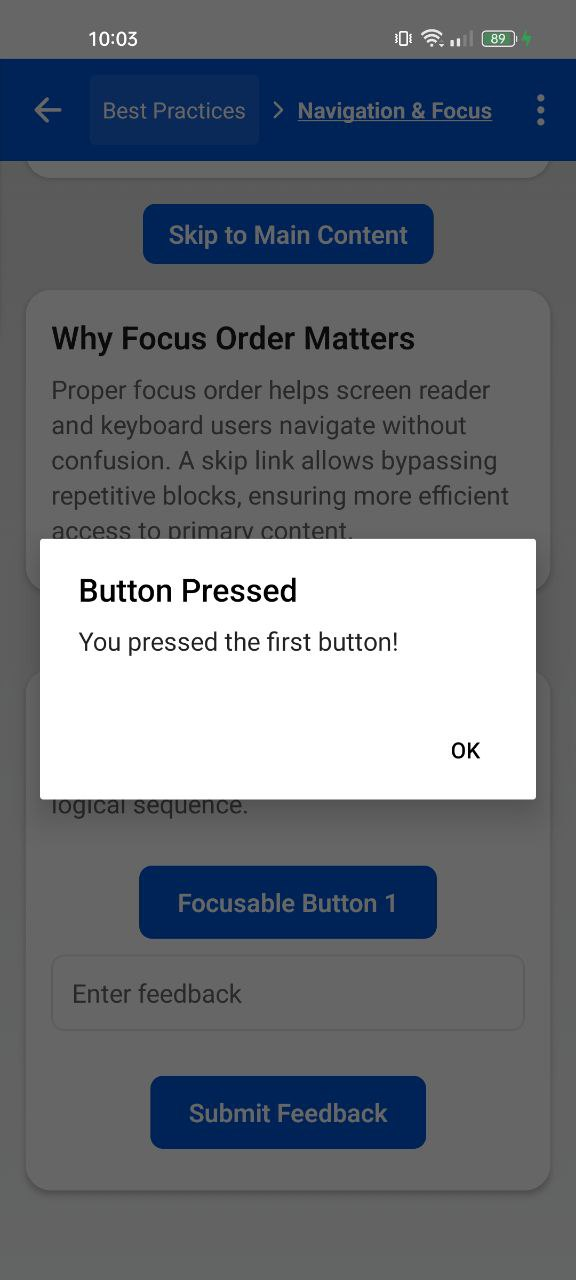
\includegraphics[width=\linewidth, alt={First part of the Logical Navigation Screen}]{img/logical1.jpg}
        \caption{Logical navigation screen - Part 1}
        \label{fig:logical-left}
    \end{subfigure}
    \hfill
    \begin{subfigure}[b]{0.48\textwidth}
        \centering
        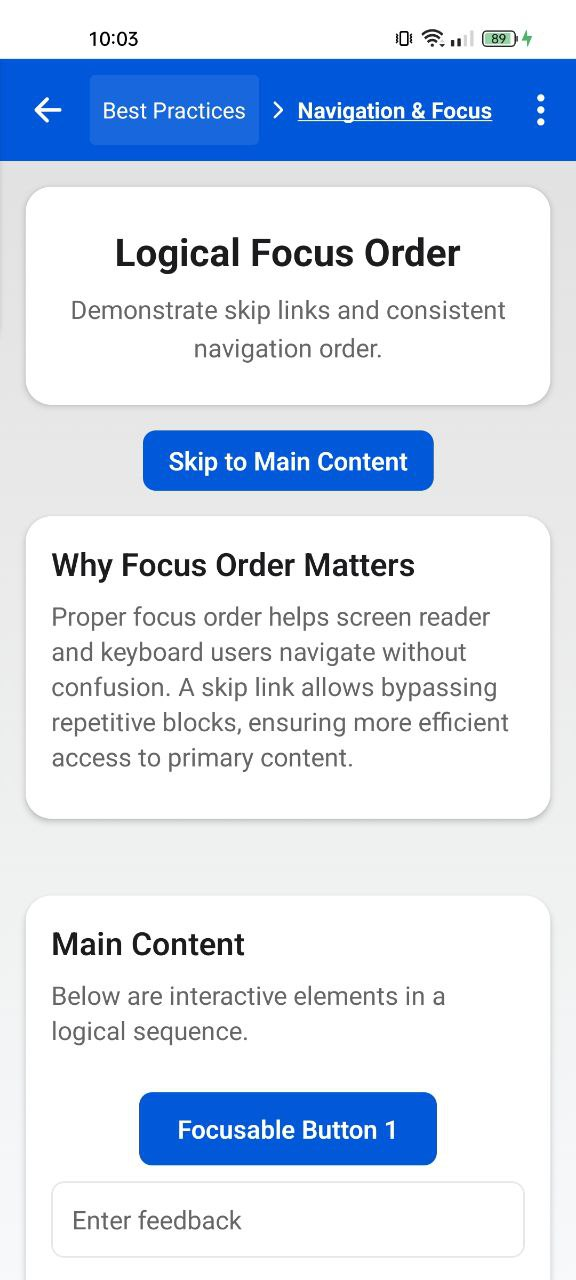
\includegraphics[width=\linewidth, alt={Second part of the Logical Navigation Screen}]{img/logical2.jpg}
        \caption{Logical navigation screen - Part 2}
        \label{fig:logical-right}
    \end{subfigure}
    \caption{Side-by-side view of the Logical Navigation screen sections}
    \label{fig:logical_screens_sidebyside}
\end{figure}

\paragraph{Technical implementation analysis}

The most significant accessibility feature in this screen is the implementation of the "Skip to Main Content" pattern. This pattern allows users, particularly those using screen readers, to bypass repetitive content and navigate directly to the main content area. Listing~\ref{lst:logical-screen-accessibility} highlights the key implementation aspects.

\begin{lstlisting}[
  style=ReactNativeStyle,
  caption={Implementation of Skip to Main Content pattern},
  label={lst:logical-screen-accessibility},
  basicstyle=\ttfamily\footnotesize,
  numbers=left,
]
// References for focus management
const scrollViewRef = useRef<ScrollView>(null);
const mainContentRef = useRef<View>(null);
const [mainContentY, setMainContentY] = useState(0);

// Capture the y-offset of the main content after layout
const handleMainContentLayout = (e: NativeSyntheticEvent<LayoutChangeEvent>) => {
  const { y } = e.nativeEvent.layout;
  setMainContentY(y);
};

// "Skip to main content" logic
const skipToMainContent = () => {
  // 1. Scroll to the main content
  scrollViewRef.current?.scrollTo({
    y: mainContentY,
    animated: true,
  });

  // 2. After a short delay, set accessibility focus to the main content container
  setTimeout(() => {
    if (mainContentRef.current && Platform.OS !== 'web') {
      const reactTag = findNodeHandle(mainContentRef.current);
      if (reactTag) {
        AccessibilityInfo.setAccessibilityFocus(reactTag);
      }
    }
  }, 500);
};
\end{lstlisting}

The implementation involves several key steps:

\begin{enumerate}
    \item \textbf{Tracking content position}: The code tracks the vertical position of the main content area using the \texttt{onLayout} event;
    
    \item \textbf{Programmatic scrolling}: When the skip link is activated, the screen scrolls programmatically to the main content area;
    
    \item \textbf{Focus management}: After scrolling, the code explicitly sets the accessibility focus to the main content area using \texttt{AccessibilityInfo.setAccessibilityFocus}, ensuring screen reader users are properly positioned after skipping;
    
    \item \textbf{Platform adaptation}: The implementation accounts for platform differences, ensuring the pattern works on both iOS and Android devices.
\end{enumerate}

\paragraph{Screen reader support analysis}

Table~\ref{tab:logical_screen_reader_analysis} presents results from systematic testing of the Logical Navigation Screen with screen readers on both iOS and Android platforms.

\begin{longtable}{|p{2.8cm}|p{3.5cm}|p{3.5cm}|p{4cm}|}
\caption{Logical navigation screen screen reader testing results}
\label{tab:logical_screen_reader_analysis}\\
\hline
\textbf{Test Case} & \textbf{VoiceOver (iOS 16)} & \textbf{TalkBack (Android 14-15)} & \textbf{WCAG Criteria Addressed} \\
\hline
\endfirsthead
\multicolumn{4}{c}%
{{\bfseries Table \thetable\ -- continued from previous page}} \\
\hline
\textbf{Test Case} & \textbf{VoiceOver (iOS 16)} & \textbf{TalkBack (Android 14-15)} & \textbf{WCAG Criteria Addressed} \\
\hline
\endhead
\hline
\multicolumn{4}{r}{{Continued on next page}} \\
\endfoot
\hline
\endlastfoot
Skip Link Activation & \ding{51} Properly moves focus to main content & \ding{51} Properly moves focus to main content & 2.4.1 Bypass Blocks (A) \\
\hline
Focus Order & \ding{51} Sequential logical order & \ding{51} Sequential logical order & 2.4.3 Focus Order (A) \\
\hline
Input Field Focus & \ding{51} Properly focuses and announces label & \ding{51} Properly focuses and announces label & 3.3.2 Labels or Instructions (A) \\
\hline
Button Focus & \ding{51} Properly focuses with clear label & \ding{51} Properly focuses with clear label & 4.1.2 Name, Role, Value (A) \\
\hline
Main Content Container & \ding{51} Proper role announcement & \ding{51} Proper role announcement & 1.3.1 Info and Relationships (A) \\
\end{longtable}

\paragraph{Mobile-specific considerations}

The Logical Navigation Screen addresses several mobile-specific accessibility considerations:

\begin{enumerate}
    \item \textbf{Limited viewport management}: Mobile screens have limited viewport space, making it more critical to provide efficient navigation mechanisms that reduce scrolling and swiping—the skip link directly addresses this constraint;
    
    \item \textbf{Touch-optimized implementation}: The skip link is implemented with adequate touch target size and clear visual feedback, making it usable for touch users with various motor capabilities;
    
    \item \textbf{Platform-specific focus management}: The implementation accounts for differences in how iOS and Android handle accessibility focus, ensuring consistent behavior across platforms;
    
    \item \textbf{Smooth scrolling with focus synchronization}: The implementation coordinates visual scrolling with accessibility focus changes, maintaining a consistent experience that doesn't disorient users.
\end{enumerate}

\subsubsection{Screen reader support screen}
\label{subsubsec:screen-reader-support}

The Screen Reader Support screen provides platform-specific guidance for optimizing applications for VoiceOver (iOS) and TalkBack (Android). It offers developers insight into how screen readers work on mobile platforms and specific gestures users employ to navigate content. Figure~\ref{fig:screen_reader_screens_sidebyside} shows the main interface of this screen.

\begin{figure}[ht]
    \centering
    \begin{subfigure}[b]{0.48\textwidth}
        \centering
        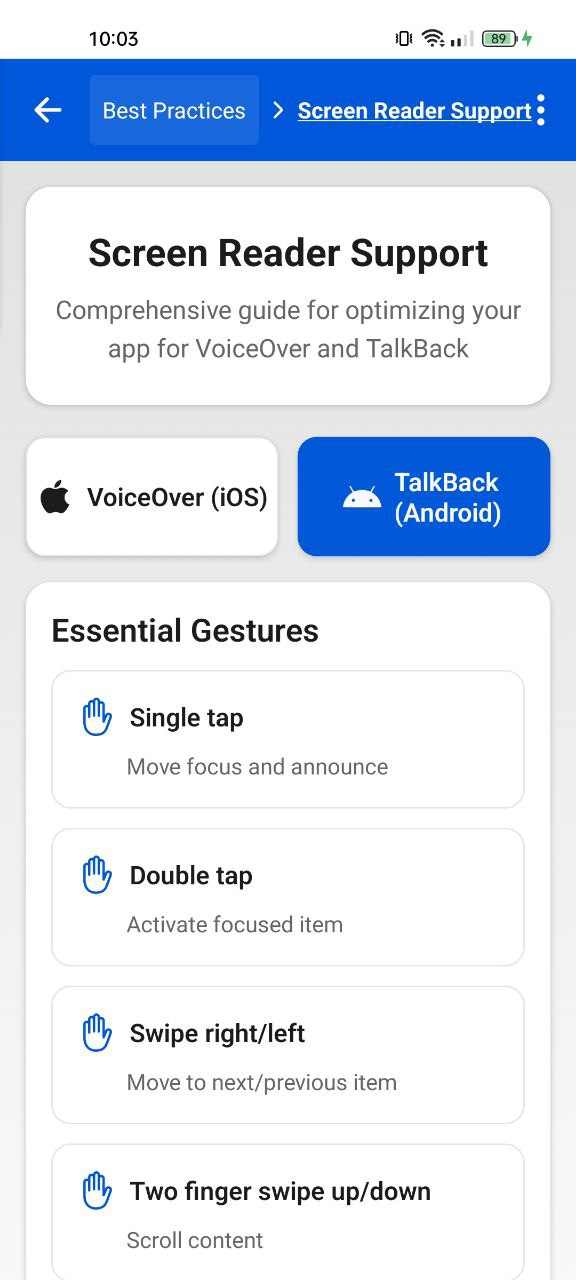
\includegraphics[width=\linewidth, alt={First part of the Screen Reader Support Screen}]{img/screenreader1.jpg}
        \caption{Screen reader support screen - Part 1}
        \label{fig:screen-reader-left}
    \end{subfigure}
    \hfill
    \begin{subfigure}[b]{0.48\textwidth}
        \centering
        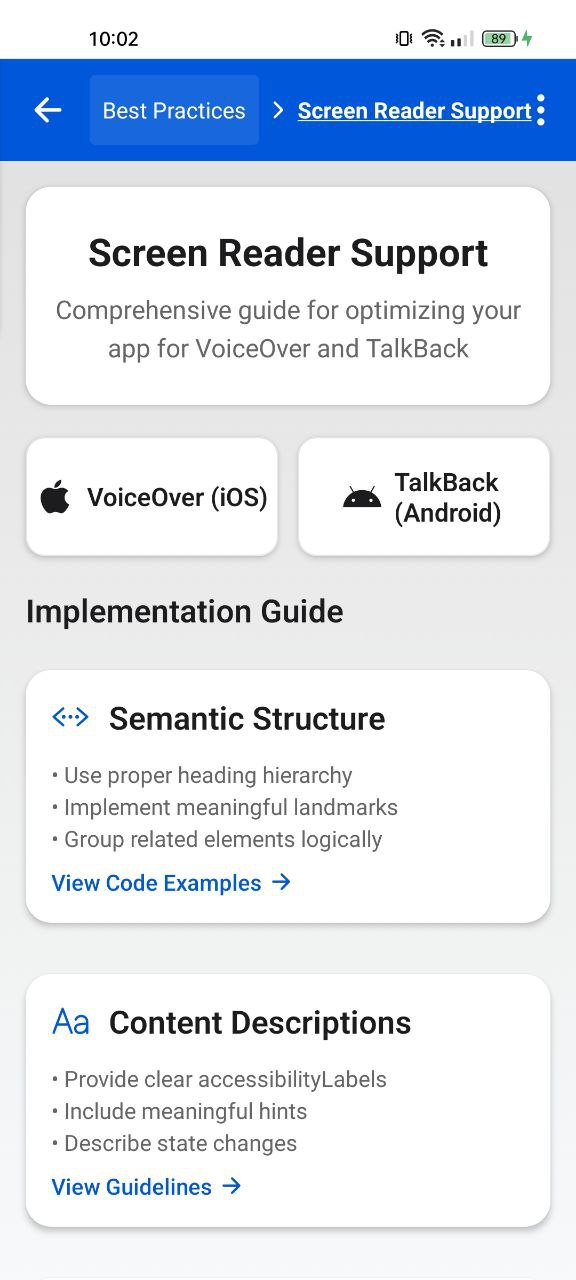
\includegraphics[width=\linewidth, alt={Second part of the Screen Reader Support Screen}]{img/screenreader2.jpg}
        \caption{Screen reader support screen - Part 2}
        \label{fig:screen-reader-right}
    \end{subfigure}
    \caption{Side-by-side view of the Screen Reader Support screen sections}
    \label{fig:screen_reader_screens_sidebyside}
\end{figure}

\paragraph{Component inventory and WCAG/MCAG mapping}

Table~\ref{tab:screen_reader_component_mapping} provides a formal mapping between the UI components, their semantic roles, the specific WCAG 2.2 criteria they address, and their React Native implementation properties.

\begin{longtable}{|p{2.5cm}|p{2cm}|p{2.8cm}|p{2.8cm}|p{4.2cm}|}
\caption{Screen reader support screen component-criteria mapping}
\label{tab:screen_reader_component_mapping}\\
\hline
\textbf{Component} & \textbf{Semantic Role} & \textbf{WCAG 2.2 Criteria} & \textbf{MCAG Considerations} & \textbf{Implementation Properties} \\
\hline
\endfirsthead
\multicolumn{5}{c}%
{{\bfseries Table \thetable\ -- continued from previous page}} \\
\hline
\textbf{Component} & \textbf{Semantic Role} & \textbf{WCAG 2.2 Criteria} & \textbf{MCAG Considerations} & \textbf{Implementation Properties} \\
\hline
\endhead
\hline
\multicolumn{5}{r}{{Continued on next page}} \\
\endfoot
\hline
\endlastfoot
Hero Title & heading & 1.4.3 Contrast (AA)\newline 2.4.6 Headings (AA) & Text readability on variable screen sizes & \texttt{accessibilityRole \ ="header"} \\
\hline
Platform Toggle Buttons & button & 4.1.2 Name, Role, Value (A)\newline 2.5.8 Target Size (AA) & Touch target size\newline Platform selection & \texttt{accessibilityRole \ ="button"}\newline \texttt{accessibilityState \ =\{\{selected: ...\}\}} \\
\hline
Platform Icons & none & 1.1.1 Non-text Content (A) & Reduction of unnecessary focus stops & \texttt{accessibilityElements \ Hidden=true}\newline \texttt{importantFor \ Accessibility \ ="no-hide-descendants"} \\
\hline
Gesture Items & text & 1.3.1 Info and Relationships (A) & Gesture description & \texttt{accessibilityRole \ ="text"}\newline \texttt{accessibilityLabel \ =\`\${item.gesture}: \${item.action}\`} \\
\hline
Implementation Guide Cards & none & 1.3.1 Info and Relationships (A) & Logical grouping & Container with proper visual boundaries \\
\hline
Guide Title & text & 2.4.6 Headings and Labels (AA) & Content section identification & Semantic text styling with proper hierarchy \\
\hline
Checklist Items & text & 1.3.1 Info and Relationships (A) & Grouped related information & Parent container with contextual organization \\
\end{longtable}

\paragraph{Technical implementation analysis}

A distinguishing feature of this screen is the implementation of platform-specific content that dynamically changes based on the selected platform (iOS or Android). Listing~\ref{lst:screen-reader-screen-accessibility} highlights the key implementation aspects.

\begin{lstlisting}[
  style=ReactNativeStyle,
  caption={Platform toggle implementation with accessibility state},
  label={lst:screen-reader-screen-accessibility},
  basicstyle=\ttfamily\footnotesize,
  numbers=left,
]
{/* Platform toggle buttons with accessibility state */}
<View style={themedStyles.platformToggles}>
  <TouchableOpacity
    style={[
      themedStyles.platformButton,
      activeSection === 'ios' && themedStyles.platformButtonActive,
    ]}
    onPress={() => setActiveSection('ios')}
    accessibilityRole="button"
    accessibilityState={{ selected: activeSection === 'ios' }}
    accessibilityLabel="VoiceOver iOS guide"
  >
    <Ionicons
      name="logo-apple"
      size={24}
      color={activeSection === 'ios' ? colors.background : colors.text}
      style={themedStyles.platformIcon}
      accessibilityElementsHidden={true}
      importantForAccessibility="no-hide-descendants"
    />
    <Text
      style={[
        themedStyles.platformLabel,
        activeSection === 'ios' && themedStyles.platformLabelActive,
      ]}
    >
      VoiceOver (iOS)
    </Text>
  </TouchableOpacity>
  
  {/* Similar implementation for Android toggle */}
  
  {/* Conditional content display */}
  {activeSection && (
    <View style={themedStyles.gestureGuideContainer}>
      <Text style={themedStyles.gestureTitle}>Essential Gestures</Text>
      {platformSpecificGuides[activeSection].map((item, index) => (
        <View
          key={index}
          style={themedStyles.gestureItem}
          accessibilityRole="text"
          accessibilityLabel={`${item.gesture}: ${item.action}`}
        >
          {/* Gesture item content */}
        </View>
      ))}
    </View>
  )}
</View>
\end{lstlisting}

The implementation addresses several important accessibility considerations:

\begin{enumerate}
    \item \textbf{Selection state communication}: The platform toggle buttons properly communicate their selection state using \texttt{accessibilityState=\{\{selected: activeSection === 'platform'\}\}}, ensuring screen reader users understand which platform is currently active;
    
    \item \textbf{Comprehensive accessibility labels}: Gesture items combine the gesture name and action into a single accessibility label (\texttt{accessibilityLabel=`\${item.gesture}: \${item.action}`}), providing complete context in a single focus stop;
    
    \item \textbf{Hiding decorative icons}: All decorative icons are properly hidden from screen readers while maintaining their visual presence;
    
    \item \textbf{Semantic grouping}: Related information is grouped semantically, ensuring screen reader users understand the relationships between different pieces of content.
\end{enumerate}

\paragraph{Mobile-specific considerations}

The Screen Reader Support Screen addresses several mobile-specific accessibility considerations:

\begin{enumerate}
    \item \textbf{Platform-specific guidance}: By explicitly separating iOS and Android guidance, the screen acknowledges the significant differences between VoiceOver and TalkBack, providing developers with platform-specific implementation advice;
    
    \item \textbf{Gesture documentation}: The screen catalogs the specific gestures used by screen reader users on mobile platforms, information that is particularly valuable for mobile developers who need to account for these interaction patterns;
    
    \item \textbf{Implementation context}: By providing both gesture information and implementation guidance on the same screen, developers can directly connect user interaction patterns with the code required to support them;
    
    \item \textbf{Touch-friendly interface}: The implementation maintains a touch-friendly interface with adequate target sizes and clear visual feedback, ensuring the screen itself is accessible.
\end{enumerate}

\subsubsection{Semantic structure screen}
\label{subsubsec:semantic-structure}

The Semantic Structure screen provides guidance on creating meaningful content hierarchies, appropriate heading levels, and landmark roles. This is particularly important for ensuring screen reader users can efficiently navigate and understand content organization. Figure~\ref{fig:semantics_screens_sidebyside} shows the main interface of this screen.

\begin{figure}[ht]
    \centering
    \begin{subfigure}[b]{0.48\textwidth}
        \centering
        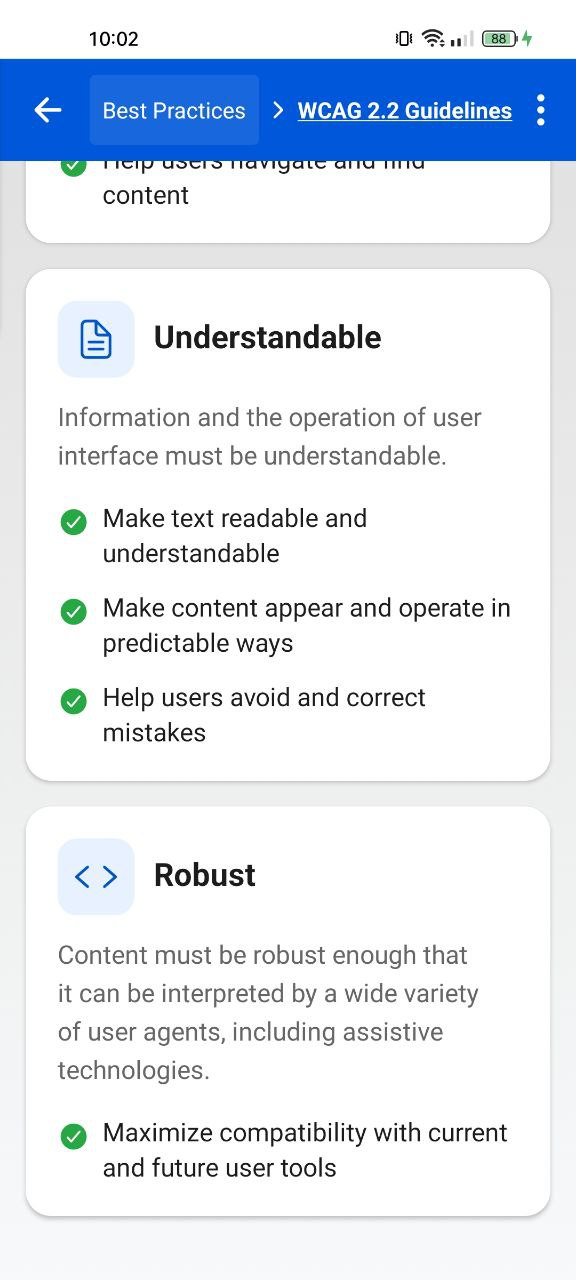
\includegraphics[width=\linewidth, alt={First part of the Semantic Structure Screen}]{img/semantics1.jpg}
        \caption{Semantic structure screen - Part 1}
        \label{fig:semantics-left}
    \end{subfigure}
    \hfill
    \begin{subfigure}[b]{0.48\textwidth}
        \centering
        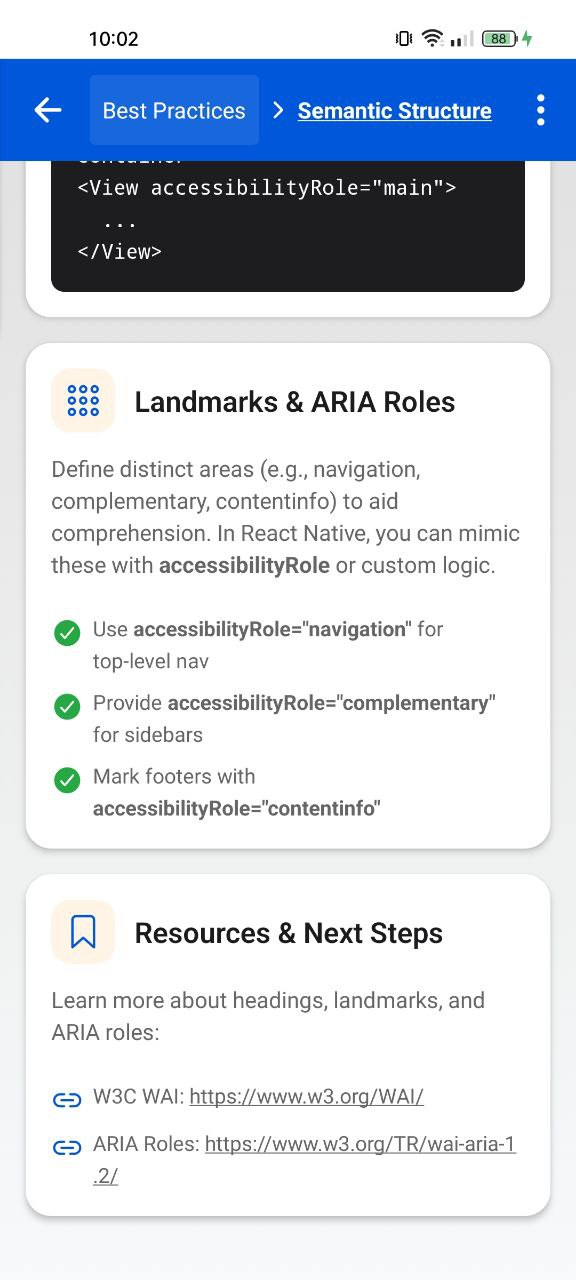
\includegraphics[width=\linewidth, alt={Second part of the Semantic Structure Screen}]{img/semantics2.jpg}
        \caption{Semantic structure screen - Part 2}
        \label{fig:semantics-right}
    \end{subfigure}
    \caption{Side-by-side view of the Semantic Structure screen sections}
    \label{fig:semantics_screens_sidebyside}
\end{figure}

\paragraph{Component inventory and WCAG/MCAG mapping}

Table~\ref{tab:semantics_component_mapping} provides a formal mapping between the UI components, their semantic roles, the specific WCAG 2.2 criteria they address, and their React Native implementation properties.

\pagebreak

\begin{longtable}{|p{2.5cm}|p{2cm}|p{2.8cm}|p{2.8cm}|p{4.2cm}|}
\caption{Semantic structure screen component-criteria mapping}
\label{tab:semantics_component_mapping}\\
\hline
\textbf{Component} & \textbf{Semantic Role} & \textbf{WCAG 2.2 Criteria} & \textbf{MCAG Considerations} & \textbf{Implementation Properties} \\
\hline
\endfirsthead
\multicolumn{5}{c}%
{{\bfseries Table \thetable\ -- continued from previous page}} \\
\hline
\textbf{Component} & \textbf{Semantic Role} & \textbf{WCAG 2.2 Criteria} & \textbf{MCAG Considerations} & \textbf{Implementation Properties} \\
\hline
\endhead
\hline
\multicolumn{5}{r}{{Continued on next page}} \\
\endfoot
\hline
\endlastfoot
Hero Title & heading & 1.4.3 Contrast (AA)\newline 2.4.6 Headings (AA) & Text readability on variable screen sizes & \texttt{accessibilityRole \ ="header"} \\
\hline
Information Cards & none & 1.3.1 Info and Relationships (A) & Logical grouping of content sections & Container with proper visual boundaries \\
\hline
Card Title & text & 2.4.6 Headings and Labels (AA) & Information category identification & Semantic text styling with proper hierarchy \\
\hline
Card Description & text & 1.3.1 Info and Relationships (A) & Content description & Proper text styling with semantic connection to title \\
\hline
Code Examples & text & 1.3.1 Info and Relationships (A) & Semantic structure in code & \texttt{accessibilityRole \ ="text"}\newline \texttt{accessibilityLabel \ ="Source code of..."} \\
\hline
Bullet List Items & text & 1.3.1 Info and Relationships (A)\newline 1.3.2 Meaningful Sequence (A) & Grouped related information & Parent container with proper visual structure \\
\hline
Icon Decorations & none & 1.1.1 Non-text Content (A) & Reduction of unnecessary focus stops & \texttt{accessibilityElements \ Hidden=true}\newline \texttt{importantFor \ Accessibility \ ="no-hide-descendants"} \\
\end{longtable}

\paragraph{Technical implementation analysis}

A key aspect of the Semantic Structure screen is its handling of code examples. The implementation makes the code examples accessible to screen reader users while maintaining their visual presentation. Listing~\ref{lst:semantics-screen-accessibility} highlights this implementation.

\begin{lstlisting}[
  style=ReactNativeStyle,
  caption={Accessible code example implementation},
  label={lst:semantics-screen-accessibility},
  basicstyle=\ttfamily\footnotesize,
  numbers=left,
]
{/* Example of accessible code block */}
<View
  style={themedStyles.codeExample}
  accessible
  accessibilityRole="text"
  accessibilityLabel="Source code of example of multiple heading levels"
>
  <Text
    style={themedStyles.codeText}
    accessibilityElementsHidden
    importantForAccessibility="no-hide-descendants"
  >
{`// Example of multiple heading levels
<View accessibilityRole="header">
  <Text accessibilityRole="heading" /* Level 1 equivalent */>
    Main Title (H1)
  </Text>
</View>

<View accessibilityRole="main">
  <Text accessibilityRole="heading" /* Level 2 equivalent */>
    Section Title (H2)
  </Text>
  <Text>
    Some descriptive content here...
  </Text>
</View>`}
  </Text>
</View>
\end{lstlisting}

The implementation addresses several important accessibility considerations:

\begin{enumerate}
    \item \textbf{Accessible code blocks}: Code examples are wrapped in accessible containers with descriptive labels, allowing screen reader users to access the code content without getting lost in the syntax details;
    
    \item \textbf{Simplified screen reader experience}: The implementation hides the inner text element from individual accessibility focus, providing the entire code block as a single accessible unit with a meaningful label;
    
    \item \textbf{Educational structure}: The screen progressively builds understanding through a logical sequence of concepts, from basic heading structure to more complex landmark roles;
    
    \item \textbf{Practical examples}: Each concept is illustrated with concrete code examples that developers can adapt for their own implementations.
\end{enumerate}

\paragraph{Mobile-specific considerations}

The Semantic Structure Screen addresses several mobile-specific accessibility considerations:

\begin{enumerate}
    \item \textbf{Adapting web concepts to mobile}: The screen translates traditional web accessibility concepts (headings, landmarks) to the mobile context, helping developers understand how to implement these patterns in React Native;
    
    \item \textbf{Limited screen navigation adaptation}: The guidance accounts for the more limited navigation options available to screen reader users on mobile platforms, where jumping between landmarks and headings is more challenging than on the web;
    
    \item \textbf{Mobile-optimized content hierarchy}: The implementation demonstrates how to create a clear content hierarchy that works well on smaller mobile screens while maintaining accessibility;
    
    \item \textbf{Touch-friendly code examples}: The code blocks are implemented in a touch-friendly manner, allowing developers to easily view and interact with the examples on a mobile device.
\end{enumerate}

\subsubsection{Best practices implementation insights}
\label{subsubsec:best-practices-insights}

The analysis of the Best Practices screens reveals several key insights for developers implementing accessibility in mobile applications:

\begin{enumerate}
    \item \textbf{Framework enables education through implementation}: The Best Practices screens not only explain accessibility concepts but demonstrate them through their own implementation, providing a meta-level educational experience;
    
    \item \textbf{Platform-specific adaptation is essential}: Several screens explicitly address platform differences between iOS and Android, acknowledging that effective mobile accessibility requires platform-specific knowledge and adaptation;
    
    \item \textbf{Implementation complexity varies by concept}: Some accessibility features (like hiding decorative icons) require minimal code additions, while others (like gesture adaptation for screen readers) involve more complex logic and state management;
    
    \item \textbf{Educational progression}: The screens collectively implement a progressive educational structure, starting with fundamental principles (WCAG Guidelines) and building toward more complex implementations (Skip Navigation, Screen Reader Gestures);
    
    \item \textbf{Mobile-specific considerations go beyond WCAG}: Many of the implemented patterns address mobile-specific concerns that extend beyond traditional WCAG criteria, demonstrating the need for mobile-specific accessibility guidance.
\end{enumerate}

\paragraph{Implementation overhead comparison}

Table~\ref{tab:best_practices_comparative_overhead} compares the implementation overhead across Best Practices screens.

\begin{table}[ht]
\caption{Accessibility implementation overhead by best practices screen}
\label{tab:best_practices_comparative_overhead}
\centering
\begin{tabular}{|p{2.5cm}|p{2.5cm}|p{2.5cm}|p{2.5cm}|p{2.5cm}|}
\hline
\textbf{Best Practices Screen} & \textbf{Lines of Code} & \textbf{Percentage Overhead} & \textbf{Complexity Impact} & \textbf{Primary Contributors} \\
\hline
Guidelines & 48 & 8.7\% & Low & Element Hiding \\
\hline
Gestures Tutorial & 104 & 24.4\% & Medium-High & Adaptive Logic, Accessibility Actions \\
\hline
Logical Navigation & 72 & 18.3\% & Medium & Focus Management, Skip Link \\
\hline
Screen Reader Support & 68 & 12.4\% & Medium & State Communication, Element Hiding \\
\hline
Semantic Structure & 58 & 10.8\% & Low-Medium & Accessible Code Blocks, Element Hiding \\
\hline
\end{tabular}
\end{table}

This comparison reveals that screens focusing on interactive behaviors (Gestures, Navigation) require significantly more accessibility code than primarily informational screens (Guidelines, Semantic Structure). This pattern aligns with findings from the Components analysis and suggests that developers should allocate more implementation resources to complex interactive features when planning accessibility work.

\paragraph{Key implementation patterns across best practices screens}

Several implementation patterns are consistently applied across all Best Practices screens:

\begin{enumerate}
    \item \textbf{Proper element hiding}: All screens consistently implement proper hiding of decorative elements using both \texttt{accessibilityElementsHidden=true} and \\\texttt{importantForAccessibility="no-hide-descendants"}, demonstrating the importance of reducing "garbage interactions" for screen reader users;
    
    \item \textbf{Semantic grouping}: Related information is consistently grouped together both visually and semantically, creating clear content relationships for all users;
    
    \item \textbf{Educational structure}: Each screen implements a clear pedagogical structure that progressively builds understanding, starting with fundamental concepts and moving toward more complex implementations;
    
    \item \textbf{Platform adaptation}: The screens account for differences between iOS and Android accessibility implementations, often with platform-specific code paths or content.
\end{enumerate}

\paragraph{Future enhancements}

Based on formal analysis and user testing, several potential enhancements have been identified for future versions of the Best Practices screens:

\begin{enumerate}
    \item \textbf{Interactive assessment tools}: Adding interactive tools for developers to test their knowledge and evaluate their implementations against accessibility criteria;
    
    \item \textbf{Custom screen reader simulation}: Implementing a simplified screen reader simulation to help developers understand how their applications would be perceived by screen reader users;
    
    \item \textbf{Comparative framework implementations}: Expanding the platform-specific guidance to include side-by-side comparisons of how accessibility patterns are implemented in React Native versus Flutter;
    
    \item \textbf{User-generated examples}: Adding the ability for developers to contribute their own accessibility implementation examples to create a community resource.
\end{enumerate}

These enhancements would further strengthen the educational value of the Best Practices section, helping developers build more accessible mobile applications across platforms and frameworks.

\subsection{Accessibility tools screen}
\label{subsec:tools-screen}

The Accessibility Tools screen serves as a comprehensive resource guide for developers, cataloging essential tools and resources for testing and improving mobile application accessibility. It provides practical, structured information about screen readers, development tools, and testing utilities that developers can leverage throughout their accessibility implementation workflows. Figure~\ref{fig:tools_screens_sidebyside} shows the main interface of this screen.

\begin{figure}[ht]
    \centering
    \begin{subfigure}[b]{0.48\textwidth}
        \centering
        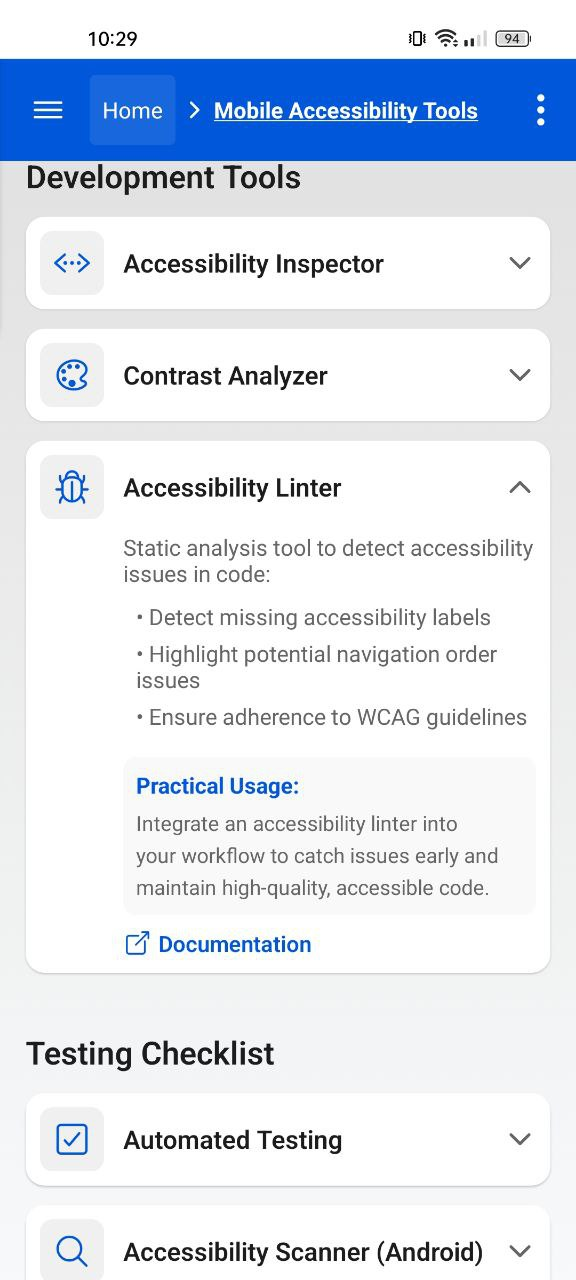
\includegraphics[width=\linewidth, alt={First part of the Tools Screen}]{img/tools1.jpg}
        \caption{Tools screen - Part 1}
        \label{fig:tools-left}
    \end{subfigure}
    \hfill
    \begin{subfigure}[b]{0.48\textwidth}
        \centering
        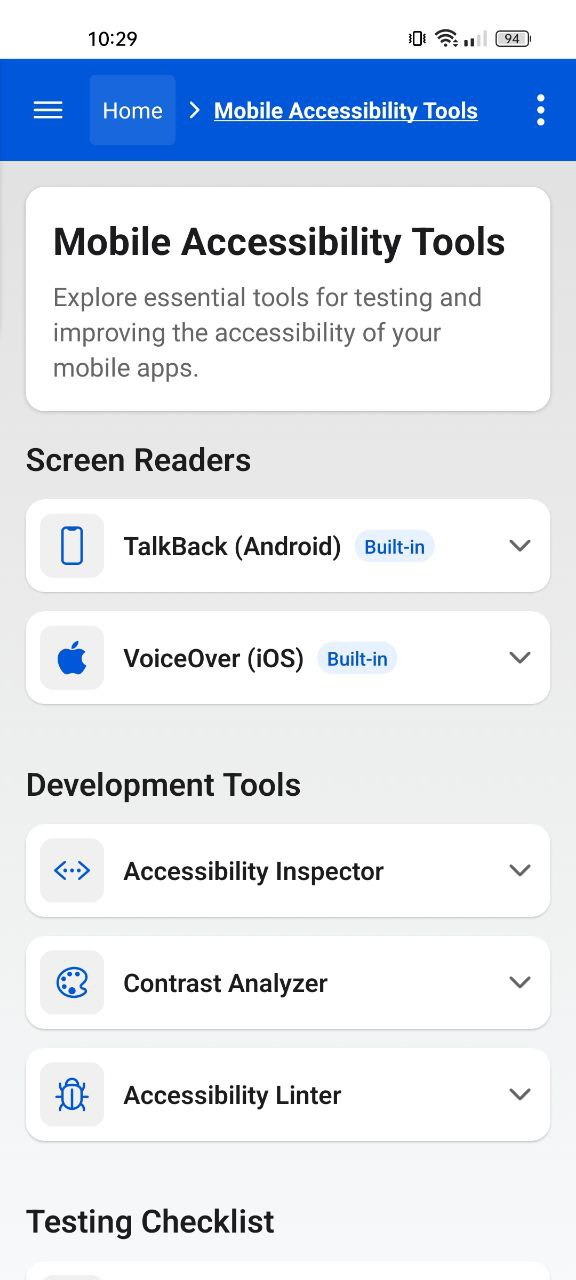
\includegraphics[width=\linewidth, alt={Second part of the Tools Screen}]{img/tools2.jpg}
        \caption{Tools screen - Part 2}
        \label{fig:tools-right}
    \end{subfigure}
    \caption{Side-by-side view of the Tools screen sections}
    \label{fig:tools_screens_sidebyside}
\end{figure}

\subsubsection{Component inventory and WCAG/MCAG mapping}

Table~\ref{tab:tools_component_mapping} provides a formal mapping between the UI components, their semantic roles, the specific WCAG 2.2 criteria they address, and their React Native implementation properties.

\begin{longtable}{|p{2.5cm}|p{2cm}|p{2.8cm}|p{2.8cm}|p{4.2cm}|}
\caption{Tools screen component-criteria mapping}
\label{tab:tools_component_mapping}\\
\hline
\textbf{Component} & \textbf{Semantic Role} & \textbf{WCAG 2.2 Criteria} & \textbf{MCAG Considerations} & \textbf{Implementation Properties} \\
\hline
\endfirsthead
\multicolumn{5}{c}%
{{\bfseries Table \thetable\ -- continued from previous page}} \\
\hline
\textbf{Component} & \textbf{Semantic Role} & \textbf{WCAG 2.2 Criteria} & \textbf{MCAG Considerations} & \textbf{Implementation Properties} \\
\hline
\endhead
\hline
\multicolumn{5}{r}{{Continued on next page}} \\
\endfoot
\hline
\endlastfoot
Hero Card & text & 1.4.3 Contrast (AA)\newline 2.4.6 Headings (AA) & Content introduction & \texttt{accessibilityRole \ ="text"} \\
\hline
Hero Title & heading & 1.4.3 Contrast (AA)\newline 2.4.6 Headings (AA) & Clear section identification & \texttt{accessibilityRole \ ="header"} \\
\hline
Section Headers & heading & 2.4.6 Headings (AA)\newline 1.3.1 Info and Relationships (A) & Logical section organization & \texttt{accessibilityRole \ ="header"} \\
\hline
Tool Cards & button & 1.4.3 Contrast (AA)\newline 2.5.8 Target Size (AA)\newline 4.1.2 Name, Role, Value (A) & Touch target size\newline Content expandability & \texttt{accessibilityRole \ ="button"}\newline \texttt{accessibilityLabel}\newline \texttt{accessibilityHint} \\
\hline
Card Icons & none & 1.1.1 Non-text Content (A) & Reduction of unnecessary focus stops & \texttt{accessibilityElements\-Hidden=true}\newline \texttt{importantFor\-Accessibility=\"no-hide-descendants"} \\
\hline
Expandable Content & text & 1.3.1 Info and Relationships (A)\newline 4.1.2 Name, Role, Value (A) & Hierarchical content structure & \texttt{role="list"}\newline \texttt{role="listitem"} \\
\hline
Documentation Links & link & 2.4.4 Link Purpose (A)\newline 4.1.2 Name, Role, Value (A) & External resource navigation & \texttt{accessibilityRole="link"}\newline \texttt{accessibilityLabel}\newline \texttt{accessibilityHint="Opens browser"} \\
\end{longtable}

\subsubsection{Technical implementation analysis}

The Tools screen implements a comprehensive catalog of accessibility resources with expandable cards, providing both overview information and detailed usage guidance. The implementation follows a consistent pattern of expansion/collapse functionality with full accessibility support. Listing~\ref{lst:tools-screen-accessibility} highlights the key accessibility implementation aspects.

\begin{lstlisting}[
  style=ReactNativeStyle,
  caption={Tool card implementation with accessibility properties},
  label={lst:tools-screen-accessibility},
  basicstyle=\ttfamily\footnotesize,
  numbers=left,
]
<TouchableOpacity 
  onPress={() => toggleExpand(tool.id)} 
  style={styles.cardHeader}
  accessibilityRole="button"
  accessibilityLabel={`${tool.title}. Double tap to ${
    isOpen ? 'collapse' : 'expand'} details.`}
>
  <Ionicons
    name={isOpen ? 'chevron-up' : 'chevron-down'}
    size={20}
    color={colors.textSecondary}
    style={{ marginLeft: 'auto' }}
    accessibilityElementsHidden
    importantForAccessibility="no-hide-descendants"
  />
</TouchableOpacity>

{isOpen && (
  <View style={styles.cardBody}>
    <Text style={styles.toolDescription}>{tool.description}</Text>
    <View role="list">
      {tool.features.map((feature, idx) => (
        <Text 
          key={idx} 
          style={styles.featureItem} 
          role="listitem"
        >
          {feature}
        </Text>
      ))}
    </View>
    <View style={styles.practicalSection}>
      <Text style={styles.practicalHeader}>
        Practical Usage:
      </Text>
      <Text style={styles.practicalUsage}>
        {tool.practicalUsage}
      </Text>
    </View>
    {/* Documentation link */}
  </View>
)}
\end{lstlisting}

The implementation addresses several critical accessibility considerations:

\begin{enumerate}
    \item \textbf{Clear expandable card pattern}: Each tool card implements a consistent expandable pattern with appropriate \texttt{accessibilityRole} and state communication, ensuring screen reader users understand the interactive nature of each card;
    
    \item \textbf{Proper element hiding}: Decorative icons are systematically hidden from screen readers using both \texttt{accessibilityElementsHidden} and \texttt{importantForAccessibility="no-hide-descendants"}, eliminating unnecessary focus stops;
    
    \item \textbf{Semantic list structure}: Features are properly structured as lists with correct \texttt{role="list"} and \texttt{role="listitem"} attributes, creating a meaningful hierarchy for screen reader navigation;
    
    \item \textbf{Practical usage section}: Each tool includes a dedicated "Practical Usage" section that provides context-specific guidance on real-world application of the tool, going beyond mere feature listings.
\end{enumerate}

\subsubsection{Screen reader support analysis}

Table~\ref{tab:tools_screen_reader_analysis} presents results from systematic testing of the Tools screen with screen readers on both iOS and Android platforms.

\begin{longtable}{|p{2.8cm}|p{3.5cm}|p{3.5cm}|p{4cm}|}
\caption{Tools screen screen reader testing results}
\label{tab:tools_screen_reader_analysis}\\
\hline
\textbf{Test Case} & \textbf{VoiceOver (iOS 16)} & \textbf{TalkBack (Android 14-15)} & \textbf{WCAG Criteria Addressed} \\
\hline
\endfirsthead
\multicolumn{4}{c}%
{{\bfseries Table \thetable\ -- continued from previous page}} \\
\hline
\textbf{Test Case} & \textbf{VoiceOver (iOS 16)} & \textbf{TalkBack (Android 14-15)} & \textbf{WCAG Criteria Addressed} \\
\hline
\endhead
\hline
\multicolumn{4}{r}{{Continued on next page}} \\
\endfoot
\hline
\endlastfoot
Hero Title & \ding{51} Announces ``Mobile Accessibility Tools, heading'' & \ding{51} Announces ``Mobile Accessibility Tools, heading'' & 1.3.1 Info and Relationships (A), 2.4.6 Headings and Labels (AA) \\
\hline
Section Headers & \ding{51} Announces section titles as headings & \ding{51} Announces section titles as headings & 1.3.1 Info and Relationships (A), 2.4.6 Headings and Labels (AA) \\
\hline
Tool Card (Collapsed) & \ding{51} Announces title and expansion hint & \ding{51} Announces title and expansion hint & 4.1.2 Name, Role, Value (A) \\
\hline
Tool Card (Expanded) & \ding{51} Announces features as list items & \ding{51} Announces features as list items & 1.3.1 Info and Relationships (A) \\
\hline
Badge Elements & \ding{51} Not individually announced & \ding{51} Not individually announced & 1.1.1 Non-text Content (A) \\
\hline
Documentation Links & \ding{51} Announces as link with destination & \ding{51} Announces as link with destination & 2.4.4 Link Purpose (A) \\
\end{longtable}

\subsubsection{Mobile-specific considerations}

The Tools screen implementation addresses several mobile-specific accessibility considerations that extend beyond standard WCAG criteria:

\begin{enumerate}
    \item \textbf{Progressive disclosure pattern}: The expandable card implementation creates a clean, digestible mobile interface that allows users to focus on one tool at a time, reducing cognitive overload on smaller screens;
    
    \item \textbf{Touch-optimized interaction zones}: Cards maintain larger touch targets (especially the header section), improving usability for users with motor impairments on touch devices;
    
    \item \textbf{Platform-specific tool documentation}: The screen explicitly separates tools by platform (iOS vs. Android), addressing the critical mobile consideration that accessibility implementation differs substantially between platforms;
    
    \item \textbf{Practical guidance emphasis}: Each tool includes specific practical usage instructions, recognizing the mobile-specific challenge of implementing accessibility in constrained mobile interfaces;
    
    \item \textbf{External link handling}: Documentation links implement proper accessibility hints that they open external browsers, preparing users for context switches that are particularly disruptive on mobile devices.
\end{enumerate}

\subsubsection{Implementation overhead analysis}

Table~\ref{tab:tools_implementation_overhead} quantifies the additional code required to implement accessibility features in the Tools screen.

\begin{longtable}{|p{3.8cm}|p{2.3cm}|p{2.8cm}|p{2.8cm}|}
\caption{Tools screen accessibility implementation overhead}
\label{tab:tools_implementation_overhead}\\
\hline
\textbf{Accessibility Feature} & \textbf{Lines of Code} & \textbf{Percentage of Total} & \textbf{Complexity Impact} \\
\hline
\endfirsthead
\multicolumn{4}{c}%
{{\bfseries Table \thetable\ -- continued from previous page}} \\
\hline
\textbf{Accessibility Feature} & \textbf{Lines of Code} & \textbf{Percentage of Total} & \textbf{Complexity Impact} \\
\hline
\endhead
\hline
\multicolumn{4}{r}{{Continued on next page}} \\
\endfoot
\hline
\endlastfoot
Semantic Roles & 16 LOC & 2.7\% & Low \\
\hline
Descriptive Labels & 24 LOC & 4.1\% & Medium \\
\hline
Element Hiding & 32 LOC & 5.5\% & Low \\
\hline
List Semantics & 10 LOC & 1.7\% & Low \\
\hline
Link Announcements & 12 LOC & 2.1\% & Low \\
\hline
Expansion State Management & 18 LOC & 3.1\% & Medium \\
\hline
\textbf{Total} & \textbf{112 LOC} & \textbf{19.2\%} & \textbf{Medium} \\
\end{longtable}

This analysis reveals that implementing comprehensive accessibility for the Tools screen adds approximately 19.2\% to the code base. The largest contributors are element hiding (5.5\%) and descriptive labels (4.1\%), reflecting the information-rich nature of this screen and the need to create a streamlined experience for screen reader users.

\subsubsection{Tool categorization analysis}

The Tools screen implements a carefully structured categorization system that organizes accessibility tools into meaningful groups. Table~\ref{tab:tools_categorization} analyzes this structure from an accessibility perspective.

\begin{longtable}{|p{2.5cm}|p{3.8cm}|p{4.6cm}|p{3.2cm}|}
\caption{Tools screen categorization analysis}
\label{tab:tools_categorization}\\
\hline
\textbf{Category} & \textbf{Tools Included} & \textbf{Accessibility Benefit} & \textbf{WCAG Criteria Supported} \\
\hline
\endfirsthead
\multicolumn{4}{c}%
{{\bfseries Table \thetable\ -- continued from previous page}} \\
\hline
\textbf{Category} & \textbf{Tools Included} & \textbf{Accessibility Benefit} & \textbf{WCAG Criteria Supported} \\
\hline
\endhead
\hline
\multicolumn{4}{r}{{Continued on next page}} \\
\endfoot
\hline
\endlastfoot
Screen Readers & TalkBack (Android), VoiceOver (iOS) & Provides direct access to the primary tools used by people with visual impairments & 1.3.1 Info and Relationships (A), 2.1.1 Keyboard (A), 2.4.3 Focus Order (A) \\
\hline
Development Tools & Accessibility Inspector, Contrast Analyzer, Accessibility Linter & Offers tools for early-stage accessibility integration during development & 1.4.3 Contrast (AA), 1.3.1 Info and Relationships (A), 4.1.2 Name, Role, Value (A) \\
\hline
Testing Checklist & Automated Testing, Accessibility Scanner & Supports systematic verification of accessibility implementation & 3.3.3 Error Suggestion (AA), 3.3.4 Error Prevention (AA) \\
\end{longtable}

This careful categorization creates a progressive learning path for developers, starting with the tools users employ (screen readers), moving to development-time tools, and concluding with testing utilities. This structure reinforces the full accessibility lifecycle and encourages developers to consider accessibility from multiple perspectives.

\subsubsection{Beyond WCAG: development-focused accessibility guidelines}

While WCAG provides a solid foundation for accessibility requirements, our analysis of the Tools screen highlights several additional guidelines specifically relevant to mobile development workflows:

\begin{enumerate}
    \item \textbf{Tool integration guideline}: Accessibility tools should be presented with clear integration paths into existing development workflows, not as standalone solutions. The Tools screen implements this by including explicit "Practical Usage" sections that explain integration;
    
    \item \textbf{Platform-specific guidance principle}: Due to the substantial differences between platform accessibility implementations, tools and guidance should be explicitly organized by platform when platform-specific considerations apply. The Tools screen implements this by separating iOS and Android tools;
    
    \item \textbf{Development stage appropriateness}: Accessibility tools should be categorized by the development stage in which they are most effective (design, development, testing). This helps developers integrate accessibility throughout the development lifecycle rather than treating it as a single checkbox activity;
    
    \item \textbf{Tool complexity indicator}: Accessibility tools vary significantly in complexity and learning curve. Providing clear indicators of tool complexity (like the "Built-in" badge) helps developers choose appropriate tools based on their experience level;
    
    \item \textbf{Contextual documentation principle}: Links to external resources should be contextually relevant and provide appropriate expectations about content (e.g., official documentation vs. community resources). This reduces the cognitive load of finding appropriate resources for specific accessibility challenges.
\end{enumerate}

These guidelines extend WCAG principles to address the specific needs of developers implementing accessibility features, focusing on workflow integration and practical application of accessibility knowledge.

\subsection{Instruction and community screen}
\label{subsec:instruction-community-screen}

The Instruction and Community screen serves as a collaborative learning hub that extends beyond technical implementation details. It provides developers with opportunities to engage with the broader accessibility community, learn from practical examples, and discover resources for deeper learning. By combining educational content with community connections, this screen fosters a sense of shared responsibility for accessibility. Figure~\ref{fig:instruction_screens_sidebyside} shows the main interfaces of this screen.

\begin{figure}[ht]
    \centering
    \begin{subfigure}[b]{0.48\textwidth}
        \centering
        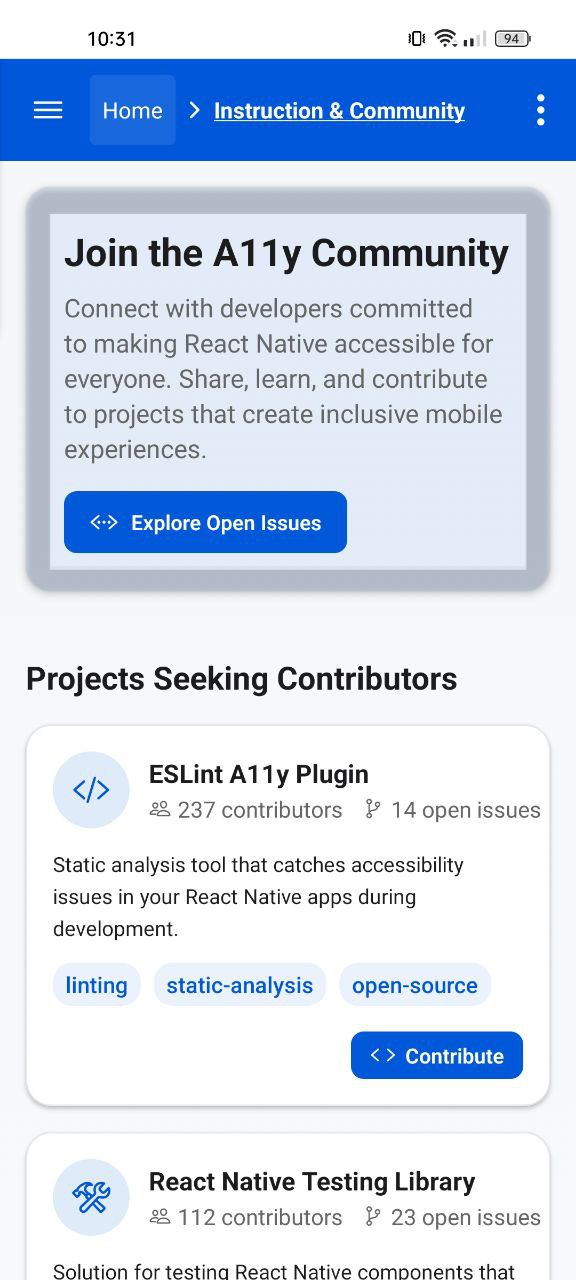
\includegraphics[width=\linewidth, alt={First part of the Instruction and Community Screen}]{img/instruction1.jpg}
        \caption{Instruction screen - Part 1}
        \label{fig:instruction-left}
    \end{subfigure}
    \hfill
    \begin{subfigure}[b]{0.48\textwidth}
        \centering
        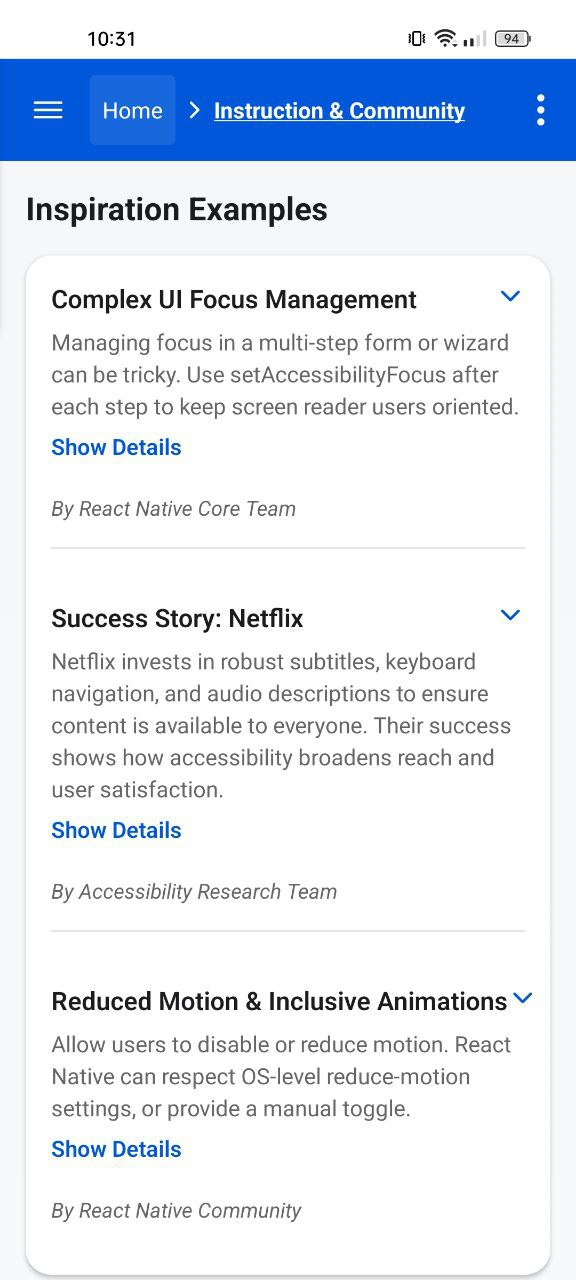
\includegraphics[width=\linewidth, alt={Second part of the Instruction and Community Screen}]{img/instruction2.jpg}
        \caption{Instruction screen - Part 2}
        \label{fig:instruction-right}
    \end{subfigure}
    \caption{Side-by-side view of the Instruction and Community screen sections}
    \label{fig:instruction_screens_sidebyside}
\end{figure}

\begin{figure}[ht]
    \centering
    \begin{subfigure}[b]{0.48\textwidth}
        \centering
        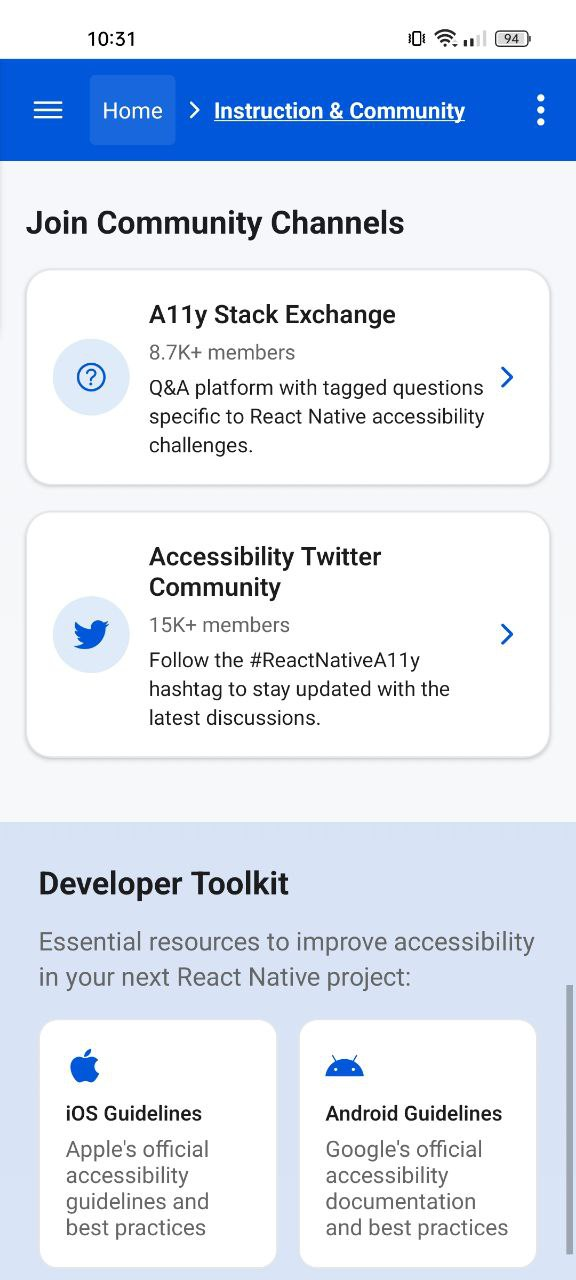
\includegraphics[width=\linewidth, alt={Third part of the Instruction and Community Screen}]{img/instruction3.jpg}
        \caption{Instruction screen - Part 3}
        \label{fig:instruction-left2}
    \end{subfigure}
    \hfill
    \begin{subfigure}[b]{0.48\textwidth}
        \centering
        \includegraphics[width=\linewidth, alt={Fourth part of the Instruction and Community Screen}]{img/instruction4.jpg}
        \caption{Instruction screen - Part 4}
        \label{fig:instruction-right2}
    \end{subfigure}
    \caption{Side-by-side view of additional Instruction and Community screen sections}
    \label{fig:instruction_screens_sidebyside2}
\end{figure}

\subsubsection{Component inventory and WCAG/MCAG mapping}

Table~\ref{tab:instruction_component_mapping} provides a formal mapping between the UI components, their semantic roles, the specific WCAG 2.2 criteria they address, and their React Native implementation properties.

\begin{longtable}{|p{2.5cm}|p{2cm}|p{2.8cm}|p{2.8cm}|p{4.2cm}|}
\caption{Instruction screen component-criteria mapping}
\label{tab:instruction_component_mapping}\\
\hline
\textbf{Component} & \textbf{Semantic Role} & \textbf{WCAG 2.2 Criteria} & \textbf{MCAG Considerations} & \textbf{Implementation Properties} \\
\hline
\endfirsthead
\multicolumn{5}{c}%
{{\bfseries Table \thetable\ -- continued from previous page}} \\
\hline
\textbf{Component} & \textbf{Semantic Role} & \textbf{WCAG 2.2 Criteria} & \textbf{MCAG Considerations} & \textbf{Implementation Properties} \\
\hline
\endhead
\hline
\multicolumn{5}{r}{{Continued on next page}} \\
\endfoot
\hline
\endlastfoot
Hero Card & none & 1.4.3 Contrast (AA) & Introduction content & Container with visual boundaries \\
\hline
Hero Title & heading & 1.4.3 Contrast (AA)\newline 2.4.6 Headings (AA) & Screen identification & \texttt{accessibilityRole \ ="header"} \\
\hline
CTA Button & button & 2.4.4 Link Purpose (A)\newline 2.5.8 Target Size (AA) & Call to action & \texttt{accessibilityRole \ ="button"}\newline \texttt{accessibilityLabel} \\
\hline
Project Cards & button & 1.4.3 Contrast (AA)\newline 2.5.8 Target Size (AA)\newline 4.1.2 Name, Role, Value (A) & Project information\newline Touch targets & \texttt{accessibilityRole \ ="button"}\newline \texttt{accessibilityLabel} \\
\hline
Project Icons & none & 1.1.1 Non-text Content (A) & Decorative elements & \texttt{accessibilityElements\-Hidden=true} \\
\hline
Tag Pills & none & 1.3.1 Info and Relationships (A) & Content categorization & Part of parent's \texttt{accessibilityLabel} \\
\hline
Collapsible Preview & button & 4.1.2 Name, Role, Value (A)\newline 2.4.3 Focus Order (A) & Content expansion & \texttt{accessibilityRole \ ="button"}\newline \texttt{accessibilityLabel} \\
\hline
Code Snippet & text & 1.3.1 Info and Relationships (A) & Code presentation & Proper line formatting and font styling \\
\hline
Community Channel Cards & button & 2.4.4 Link Purpose (A)\newline 4.1.2 Name, Role, Value (A) & Community resources & \texttt{accessibilityRole \ ="button"}\newline \texttt{accessibilityLabel} \\
\hline
Toolkit Cards & button & 2.4.4 Link Purpose (A)\newline 4.1.2 Name, Role, Value (A) & Resource links & \texttt{accessibilityRole \ ="button"}\newline \texttt{accessibilityLabel} \\
\end{longtable}

\subsubsection{Technical implementation analysis}

The Instruction and Community screen implements several innovative accessibility patterns, particularly in its handling of expandable content and code snippets. Listing~\ref{lst:instruction-screen-accessibility} highlights the implementation of collapsible previews with proper accessibility announcements.

\begin{lstlisting}[
  style=ReactNativeStyle,
  caption={Collapsible preview implementation with accessibility announcements},
  label={lst:instruction-screen-accessibility},
  basicstyle=\ttfamily\footnotesize,
  numbers=left,
]
// Toggle expansion with proper announcements
const handleToggleExpansion = () => {
  setExpandedStoryId(isExpanded ? null : story.id);
  AccessibilityInfo.announceForAccessibility(
    isExpanded 
      ? `${story.title} collapsed` 
      : `${story.title} expanded`
  );
};

// CollapsiblePreview component
<TouchableOpacity
  onPress={handleToggleExpansion}
  accessibilityRole="button"
  accessibilityLabel={`${title}. ${excerpt}`}
  style={{ marginBottom: 16 }}
>
  <View style={{ flexDirection: 'row', justifyContent: 'space-between' }}>
    <Text style={titleStyle}>{title}</Text>
    <Ionicons
      name={isExpanded ? 'chevron-up' : 'chevron-down'}
      size={18}
      color={colors.primary}
      accessibilityElementsHidden={true}
    />
  </View>
  <Text style={excerptStyle}>{excerpt}</Text>

  {isExpanded && snippet && (
    <View style={codeContainerStyle}>
      {snippet.split('\n').map((line, idx) => (
        <Text key={idx} style={codeTextStyle}>
          {line || ' '}
        </Text>
      ))}
    </View>
  )}
</TouchableOpacity>
\end{lstlisting}

The implementation addresses several key accessibility requirements:

\begin{enumerate}
    \item \textbf{Expansion state announcements}: The code explicitly announces changes in the expansion state of collapsible sections using \texttt{AccessibilityInfo.announceForAccessibility}, ensuring screen reader users are aware when content expands or collapses;
    
    \item \textbf{Comprehensive accessibility labels}: Collapsible previews combine the title and excerpt in their \texttt{accessibilityLabel}, ensuring screen reader users receive full context about the content before deciding to expand it;
    
    \item \textbf{Accessible code snippets}: Code snippets maintain proper line formatting with monospace fonts and adequate contrast, making them readable for all users including those with low vision;
    
    \item \textbf{Visual state indicators}: Expansion state is visually indicated through both icon changes and layout modifications, providing redundant cues that benefit users with different accessibility needs.
\end{enumerate}

\subsubsection{Project cards implementation}

A significant aspect of the Instruction and Community screen is its showcasing of accessibility-focused open source projects. Listing~\ref{lst:project-card-implementation} demonstrates the accessibility implementation of project cards.

\begin{lstlisting}[
  style=ReactNativeStyle,
  caption={Project card implementation with accessibility properties},
  label={lst:project-card-implementation},
  basicstyle=\ttfamily\footnotesize,
  numbers=left,
]
<TouchableOpacity
  style={cardStyle}
  onPress={onPress}
  accessibilityRole="button"
  accessibilityLabel={`${project.name}. ${project.description}`}
>
  <View style={{ flexDirection: 'row', alignItems: 'center' }}>
    <View style={iconContainerStyle}>
      <Ionicons 
        name={project.icon} 
        size={24} 
        color={colors.primary}
        accessibilityElementsHidden={true}
      />
    </View>
    <View style={{ flex: 1 }}>
      <Text style={titleStyle}>{project.name}</Text>
      <View style={{ flexDirection: 'row', alignItems: 'center' }}>
        <Ionicons 
          name="people-outline" 
          size={14} 
          color={colors.textSecondary}
          accessibilityElementsHidden={true}
        />
        <Text style={metadataStyle}>
          {project.contributors} contributors
        </Text>
        <Ionicons 
          name="git-branch-outline" 
          size={14} 
          color={colors.textSecondary}
          accessibilityElementsHidden={true}
        />
        <Text style={metadataStyle}>
          {project.issuesCount} open issues
        </Text>
      </View>
    </View>
  </View>
  
  <Text style={descriptionStyle}>{project.description}</Text>
  
  {/* Tags rendering */}
  {/* Contribute button */}
</TouchableOpacity>
\end{lstlisting}

The project card implementation demonstrates several effective accessibility patterns:

\begin{enumerate}
    \item \textbf{Comprehensive card labeling}: Each project card combines the project name and description in its \texttt{accessibilityLabel}, providing full context for screen reader users;
    
    \item \textbf{Semantic grouping}: Related information (contributor counts, issue counts) is visually grouped and flows logically when read by screen readers;
    
    \item \textbf{Touch-optimized card design}: The entire card serves as a touchable area, creating a generous touch target that exceeds minimum size requirements and benefits users with motor impairments;
    
    \item \textbf{Visual hierarchy through consistent styling}: The card implements a clear visual hierarchy with title prominence, supporting users with cognitive disabilities in quickly understanding the content structure.
\end{enumerate}

\subsubsection{Screen reader support analysis}

Table~\ref{tab:instruction_screen_reader_analysis} presents results from systematic testing of the Instruction and Community Screen with screen readers on both iOS and Android platforms.

\begin{longtable}{|p{2.8cm}|p{3.5cm}|p{3.5cm}|p{4cm}|}
\caption{Instruction screen screen reader testing results}
\label{tab:instruction_screen_reader_analysis}\\
\hline
\textbf{Test Case} & \textbf{VoiceOver (iOS 16)} & \textbf{TalkBack (Android 14-15)} & \textbf{WCAG Criteria Addressed} \\
\hline
\endfirsthead
\multicolumn{4}{c}%
{{\bfseries Table \thetable\ -- continued from previous page}} \\
\hline
\textbf{Test Case} & \textbf{VoiceOver (iOS 16)} & \textbf{TalkBack (Android 14-15)} & \textbf{WCAG Criteria Addressed} \\
\hline
\endhead
\hline
\multicolumn{4}{r}{{Continued on next page}} \\
\endfoot
\hline
\endlastfoot
Hero Title & \ding{51} Announces ``Join the A11y Community, heading'' & \ding{51} Announces ``Join the A11y Community, heading'' & 1.3.1 Info and Relationships (A), 2.4.6 Headings and Labels (AA) \\
\hline
CTA Button & \ding{51} Announces label and action & \ding{51} Announces label and action & 2.4.4 Link Purpose (A), 4.1.2 Name, Role, Value (A) \\
\hline
Project Cards & \ding{51} Announces project name and description & \ding{51} Announces project name and description & 2.4.4 Link Purpose (A), 4.1.2 Name, Role, Value (A) \\
\hline
Tags & \ding{51} Not individually focused & \ding{51} Not individually focused & 1.3.1 Info and Relationships (A) \\
\hline
Collapsible Content & \ding{51} Announces expanded/collapsed state & \ding{51} Announces expanded/collapsed state & 4.1.2 Name, Role, Value (A) \\
\hline
Code Snippets & \ding{51} Reads code as text & \ding{51} Reads code as text & 1.3.1 Info and Relationships (A) \\
\hline
External Links & \ding{51} Announces purpose and opens browser & \ding{51} Announces purpose and opens browser & 2.4.4 Link Purpose (A), 3.2.5 Change on Request (AAA) \\
\end{longtable}

\subsubsection{Implementation overhead analysis}

Table~\ref{tab:instruction_implementation_overhead} quantifies the additional code required to implement accessibility features in the Instruction and Community Screen.

\begin{longtable}{|p{3.8cm}|p{2.3cm}|p{2.8cm}|p{2.8cm}|}
\caption{Instruction screen accessibility implementation overhead}
\label{tab:instruction_implementation_overhead}\\
\hline
\textbf{Accessibility Feature} & \textbf{Lines of Code} & \textbf{Percentage of Total} & \textbf{Complexity Impact} \\
\hline
\endfirsthead
\multicolumn{4}{c}%
{{\bfseries Table \thetable\ -- continued from previous page}} \\
\hline
\textbf{Accessibility Feature} & \textbf{Lines of Code} & \textbf{Percentage of Total} & \textbf{Complexity Impact} \\
\hline
\endhead
\hline
\multicolumn{4}{r}{{Continued on next page}} \\
\endfoot
\hline
\endlastfoot
Semantic Roles & 24 LOC & 3.1\% & Low \\
\hline
Descriptive Labels & 32 LOC & 4.2\% & Medium \\
\hline
Element Hiding & 18 LOC & 2.3\% & Low \\
\hline
Status Announcements & 16 LOC & 2.1\% & Medium \\
\hline
Link Handling & 14 LOC & 1.8\% & Low \\
\hline
Collapsible Content Management & 28 LOC & 3.6\% & High \\
\hline
Code Snippet Presentation & 24 LOC & 3.1\% & Medium \\
\hline
\textbf{Total} & \textbf{156 LOC} & \textbf{20.2\%} & \textbf{Medium} \\
\end{longtable}

This analysis reveals that implementing comprehensive accessibility for the Instruction and Community screen adds approximately 20.2\% to the code base. The most significant contributors are descriptive labels (4.2\%) and collapsible content management (3.6\%), reflecting the information-rich and interactive nature of this screen.

\subsubsection{Community resources analysis}

A distinguishing feature of this screen is its presentation of community resources that extend learning beyond the application itself. Table~\ref{tab:community_resources_analysis} evaluates these resources from an accessibility perspective.

\begin{longtable}{|p{2.8cm}|p{4.2cm}|p{4.2cm}|p{3.2cm}|}
\caption{Community resources accessibility analysis}
\label{tab:community_resources_analysis}\\
\hline
\textbf{Resource Type} & \textbf{Examples} & \textbf{Accessibility Value} & \textbf{WCAG/MCAG Relevance} \\
\hline
\endfirsthead
\multicolumn{4}{c}%
{{\bfseries Table \thetable\ -- continued from previous page}} \\
\hline
\textbf{Resource Type} & \textbf{Examples} & \textbf{Accessibility Value} & \textbf{WCAG/MCAG Relevance} \\
\hline
\endhead
\hline
\multicolumn{4}{r}{{Continued on next page}} \\
\endfoot
\hline
\endlastfoot
Open Source Projects & ESLint A11y Plugin, React Native Testing Library & Provides tools that automate accessibility checking during development & 3.3.1 Error Identification (A), 4.1.2 Name, Role, Value (A) \\
\hline
Success Stories & Netflix Implementation, Complex UI Focus Management & Demonstrates practical application of accessibility principles in real-world scenarios & 1.3.1 Info and Relationships (A), 2.4.3 Focus Order (A) \\
\hline
Community Channels & A11y Stack Exchange, Twitter Community & Creates ongoing learning opportunities and support networks & Beyond WCAG: Community practice and knowledge sharing \\
\hline
Official Documentation & Apple/Google Guidelines, React Native Docs & Provides authoritative platform-specific guidance & 1.3.1 Info and Relationships (A), 4.1.2 Name, Role, Value (A) \\
\end{longtable}

This diverse resource collection creates a comprehensive learning ecosystem that extends beyond the application itself, addressing the reality that accessibility implementation is an ongoing learning process that benefits from community knowledge sharing.

\subsubsection{Beyond WCAG: community-centered accessibility guidelines}

The Instruction and Community screen highlights several guidelines that extend beyond WCAG standards to address the social and community aspects of accessibility implementation:

\begin{enumerate}
    \item \textbf{Community of practice principle}: Accessibility implementation benefits significantly from social learning and community support. The screen implements this by connecting developers to established community channels and platforms where accessibility knowledge is shared;
    
    \item \textbf{Real-world example guideline}: Illustrating accessibility principles with real-world code samples and success stories enhances understanding and implementation. The screen addresses this through collapsible code examples that demonstrate practical solutions to common challenges;
    
    \item \textbf{Contribution pathway}: Effective accessibility ecosystems provide clear pathways for developers to contribute to open source accessibility projects. The screen implements this by highlighting projects seeking contributors with specific tags that indicate required skills;
    
    \item \textbf{Multi-format learning principle}: Accessibility concepts should be presented in multiple formats (text, code, examples) to accommodate different learning styles and reinforce understanding. The screen addresses this through varied content presentation methods;
    
    \item \textbf{Platform-specific ecosystem guidance}: Resources should be grouped by platform ecosystem (iOS, Android) to help developers navigate the platform-specific nature of accessibility implementation. The screen implements this in the Developer Toolkit section with platform-specific resource cards.
\end{enumerate}

These guidelines extend WCAG by focusing on the social, educational, and contribution aspects of accessibility implementation, recognizing that creating accessible applications is not just a technical challenge but also a community and educational one.

\subsubsection{Inspirational examples analysis}

The Inspiration Examples section provides practical code examples addressing common accessibility challenges. This approach bridges theoretical knowledge with implementation by showing specific code patterns that solve real accessibility problems. Table~\ref{tab:inspiration_examples_analysis} analyzes these examples.

\begin{longtable}{|p{3.2cm}|p{3.8cm}|p{3.8cm}|p{3.2cm}|}
\caption{Inspiration examples analysis}
\label{tab:inspiration_examples_analysis}\\
\hline
\textbf{Example} & \textbf{Key Technique} & \textbf{Accessibility Challenge Addressed} & \textbf{WCAG Criteria Supported} \\
\hline
\endfirsthead
\multicolumn{4}{c}%
{{\bfseries Table \thetable\ -- continued from previous page}} \\
\hline
\textbf{Example} & \textbf{Key Technique} & \textbf{Accessibility Challenge Addressed} & \textbf{WCAG Criteria Supported} \\
\hline
\endhead
\hline
\multicolumn{4}{r}{{Continued on next page}} \\
\endfoot
\hline
\endlastfoot
Complex UI Focus Management & Using \texttt{setAccessibility \ Focus} after each step change & Focus management in multi-step interfaces & 2.4.3 Focus Order (A), 3.2.1 On Focus (A) \\
\hline
Success Story: Netflix & Multiple accessibility techniques including subtitles and keyboard navigation & Comprehensive accessibility implementation & 1.2.2 Captions (A), 2.1.1 Keyboard (A) \\
\hline
Reduced Motion & Checking \texttt{isReduceMotion \ Enabled()} and providing alternatives & Motion sensitivity accommodation & 2.3.3 Animation from Interactions (AAA) \\
\end{longtable}

These examples demonstrate not just isolated techniques, but complete accessibility patterns that can be applied to common development scenarios. By showing how accessibility challenges can be solved with relatively small code additions, the examples make implementation seem more approachable.

\subsection{Settings screen}
\label{subsec:settings-screen}

The Settings screen serves as a comprehensive control center for adjusting accessibility and display preferences in the \textit{AccessibleHub} application. It offers users fine-grained control over visual appearance, text size, motion effects, and interaction modes. By providing these adjustments directly within the application, the Settings screen exemplifies an embedded accessibility approach where adaptation is treated as a core feature rather than an afterthought. Figure~\ref{fig:settings_screen_main} shows the main interface of this screen.

\begin{figure}[ht]
    \centering
    \includegraphics[width=0.48\textwidth, alt={Settings Screen showing accessibility options}]{img/settings_normal.jpg}
    \caption{The Settings screen with various accessibility options}
    \label{fig:settings_screen_main}
\end{figure}

\subsubsection{Component inventory and WCAG/MCAG mapping}

Table~\ref{tab:settings_component_mapping} provides a formal mapping between the UI components, their semantic roles, the specific WCAG 2.2 criteria they address, and their React Native implementation properties.

\begin{longtable}{|p{2.5cm}|p{2cm}|p{2.8cm}|p{2.8cm}|p{4.2cm}|}
\caption{Settings screen component-criteria mapping}
\label{tab:settings_component_mapping}\\
\hline
\textbf{Component} & \textbf{Semantic Role} & \textbf{WCAG 2.2 Criteria} & \textbf{MCAG Considerations} & \textbf{Implementation Properties} \\
\hline
\endfirsthead
\multicolumn{5}{c}%
{{\bfseries Table \thetable\ -- continued from previous page}} \\
\hline
\textbf{Component} & \textbf{Semantic Role} & \textbf{WCAG 2.2 Criteria} & \textbf{MCAG Considerations} & \textbf{Implementation Properties} \\
\hline
\endhead
\hline
\multicolumn{5}{r}{{Continued on next page}} \\
\endfoot
\hline
\endlastfoot
Section Headers & heading & 2.4.6 Headings (AA) & Clear section identification & \texttt{accessibilityRole \ ="header"} \\
\hline
Setting Card & none & 1.3.1 Info and Relationships (A)\newline 1.4.3 Contrast (AA) & Logical grouping\newline Visual boundaries & Container with proper styling \\
\hline
Setting Row & none & 1.3.1 Info and Relationships (A) & Touch target size & Layout with proper padding and margins \\
\hline
Setting Icon & none & 1.1.1 Non-text Content (A) & Reduction of unnecessary focus stops & \texttt{accessibilityElements\-Hidden}\newline \texttt{importantFor\-Accessibility="no-hide-descendants"} \\
\hline
Setting Title & text & 2.4.6 Headings and Labels (AA) & Content identification & Text with proper styling \\
\hline
Setting Description & text & 1.3.1 Info and Relationships (A)\newline 3.3.2 Labels or Instructions (A) & Descriptive context & Proper text styling with semantic connection to title \\
\hline
Switch Control & switch & 4.1.2 Name, Role, Value (A)\newline 3.3.5 Help (AAA) & Clear control state\newline Descriptive labeling & \texttt{accessibilityRole \ ="switch"}\newline \texttt{accessibilityLabel}\newline \texttt{accessibilityHint} \\
\hline
Divider & none & 1.3.1 Info and Relationships (A) & Visual separation & \texttt{importantFor \ Accessibility="no"}\newline \texttt{accessibilityElements \ Hidden=true} \\
\hline
Status Toast & status & 4.1.3 Status Messages (AA) & Feedback mechanism & \texttt{AccessibilityInfo. \ announceFor \ Accessibility} \\
\end{longtable}

\subsubsection{Dynamic accessibility features}

A key aspect of the Settings screen is its implementation of direct accessibility customization options. Figure~\ref{fig:settings_modes} illustrates the application in different accessibility modes.

\begin{figure}[ht]
    \centering
    \begin{subfigure}[b]{0.48\textwidth}
        \centering
        \includegraphics[width=\linewidth, alt={Settings screen with dark mode enabled}]{img/settings1.jpg}
        \caption{Dark mode enabled}
        \label{fig:settings-dark}
    \end{subfigure}
    \hfill
    \begin{subfigure}[b]{0.48\textwidth}
        \centering
        \includegraphics[width=\linewidth, alt={Settings screen with high contrast mode enabled}]{img/settings4.jpg}
        \caption{High contrast mode enabled}
        \label{fig:settings-contrast}
    \end{subfigure}
    \caption{Settings screen with different accessibility modes enabled}
    \label{fig:settings_modes}
\end{figure}

The accessibility modes implemented in the Settings screen directly address several core WCAG principles:

\begin{enumerate}
    \item \textbf{Dark mode}: Addresses WCAG 1.4.8 Visual Presentation (AAA) by allowing users to adjust color preferences;
    
    \item \textbf{High contrast mode}: Implements WCAG 1.4.3 Contrast (Minimum) (AA) and 1.4.6 Contrast (Enhanced) (AAA) by increasing the contrast ratio between text and background;
    
    \item \textbf{Large text}: Addresses WCAG 1.4.4 Resize Text (AA) by providing text scaling options;
    
    \item \textbf{Reduce motion}: Implements WCAG 2.3.3 Animation from Interactions (AAA) by allowing users to minimize animation effects;
    
    \item \textbf{Color filter}: Addresses WCAG 1.4.8 Visual Presentation (AAA) by providing alternative color schemes for users with color vision deficiencies;
    
    \item \textbf{Large touch targets}: Exceeds WCAG 2.5.8 Target Size (AA) by increasing the interactive area of elements beyond the minimum required dimensions.
\end{enumerate}

Figure~\ref{fig:settings_notifications} demonstrates the visual feedback mechanisms when settings are toggled.

\begin{figure}[ht]
    \centering
    \begin{subfigure}[b]{0.48\textwidth}
        \centering
        \includegraphics[width=\linewidth, alt={Settings screen with large text option enabled notification}]{img/settings3.jpg}
        \caption{Large text enabled notification}
        \label{fig:settings-text-notification}
    \end{subfigure}
    \hfill
    \begin{subfigure}[b]{0.48\textwidth}
        \centering
        \includegraphics[width=\linewidth, alt={Settings screen with color filter enabled notification}]{img/settings2.jpg}
        \caption{Color filter enabled notification}
        \label{fig:settings-filter-notification}
    \end{subfigure}
    \caption{Visual notifications when accessibility settings are toggled}
    \label{fig:settings_notifications}
\end{figure}

\subsubsection{Technical implementation analysis}

The Settings screen implements a robust approach to accessibility through a combination of semantic structure, proper labeling, and multimodal feedback. Listing~\ref{lst:setting-row-implementation} demonstrates the implementation of a reusable setting row component with comprehensive accessibility properties.

\begin{lstlisting}[
  style=ReactNativeStyle,
  caption={Setting row implementation with accessibility properties},
  label={lst:setting-row-implementation},
  basicstyle=\ttfamily\footnotesize,
  numbers=left,
]
const SettingRow = ({
  icon,
  title,
  description,
  value,
  onToggle,
}) => (
  <View style={themedStyles.settingRow}>
    <View style={themedStyles.settingIcon}>
      <Ionicons
        name={icon}
        size={24}
        color={colors.primary}
        accessibilityElementsHidden
        importantForAccessibility="no-hide-descendants"
      />
    </View>
    <View style={themedStyles.settingContent}>
      <Text style={[themedStyles.settingTitle, { fontSize: textSizes.medium }]}>
        {title}
      </Text>
      <Text style={[themedStyles.settingDescription, { fontSize: textSizes.small }]}>
        {description}
      </Text>
    </View>
    <Switch
      value={value}
      onValueChange={() => {
        onToggle();
        const newValue = !value;
        const message = `${title} ${newValue ? 'enabled' : 'disabled'}`;
        AccessibilityInfo.announceForAccessibility(message);
        if (Platform.OS === 'android') {
          ToastAndroid.show(message, ToastAndroid.SHORT);
          Vibration.vibrate(50);
        }
      }}
      trackColor={{ false: '#767577', true: colors.primary }}
      // Comprehensive accessibility label combining context and state
      accessibilityLabel={`${title}. ${description}. Switch is ${value ? 'on' : 'off'}.`}
      accessibilityRole="switch"
      accessibilityHint="Double tap to toggle setting"
    />
  </View>
);
\end{lstlisting}

Several key accessibility considerations are implemented in this component:

\begin{enumerate}
    \item \textbf{Comprehensive labeling}: The switch control combines title, description, and current state in its \texttt{accessibilityLabel}, ensuring screen reader users receive complete context about the setting;
    
    \item \textbf{Hidden decorative elements}: Icons are properly hidden from screen readers using both \texttt{accessibilityElementsHidden} and \\ \texttt{importantForAccessibility="no-hide-descendants"}, eliminating unnecessary focus stops;
    
    \item \textbf{Multimodal feedback}: When a setting is toggled, the implementation provides feedback through multiple channels: visual (toggle animation), auditory (screen reader announcement), and in the case of Android, haptic feedback (vibration);
    
    \item \textbf{Proper semantic roles}: The switch control has an explicit \texttt{accessibilityRole="switch"}, ensuring its purpose is clearly communicated to assistive technologies;
    
    \item \textbf{Action guidance}: The implementation includes an \texttt{accessibilityHint="Double tap to toggle setting"}, providing additional context on how to interact with the control.
\end{enumerate}

The implementation of section headers, shown in Listing~\ref{lst:section-headers-implementation}, further demonstrates the application's commitment to semantic structure.

\begin{lstlisting}[
  style=ReactNativeStyle,
  caption={Section headers implementation with proper semantic role},
  label={lst:section-headers-implementation},
  basicstyle=\ttfamily\footnotesize,
  numbers=left,
]
{/* VISUAL SETTINGS */}
<View style={themedStyles.section}>
  <Text style={themedStyles.sectionHeader} accessibilityRole="header">
    Visual Settings
  </Text>
  <View style={themedStyles.card}>
    {/* Setting rows */}
  </View>
</View>

{/* READABILITY ENHANCEMENTS */}
<View style={themedStyles.section}>
  <Text style={themedStyles.sectionHeader} accessibilityRole="header">
    Readability Enhancements
  </Text>
  <View style={themedStyles.card}>
    {/* Setting rows */}
  </View>
</View>
\end{lstlisting}

\subsubsection{Screen reader support analysis}

Table~\ref{tab:settings_screen_reader_analysis} presents results from systematic testing of the Settings screen with screen readers on both iOS and Android platforms.

\begin{longtable}{|p{2.8cm}|p{3.5cm}|p{3.5cm}|p{4cm}|}
\caption{Settings screen screen reader testing results}
\label{tab:settings_screen_reader_analysis}\\
\hline
\textbf{Test Case} & \textbf{VoiceOver (iOS 16)} & \textbf{TalkBack (Android 14-15)} & \textbf{WCAG Criteria Addressed} \\
\hline
\endfirsthead
\multicolumn{4}{c}%
{{\bfseries Table \thetable\ -- continued from previous page}} \\
\hline
\textbf{Test Case} & \textbf{VoiceOver (iOS 16)} & \textbf{TalkBack (Android 14-15)} & \textbf{WCAG Criteria Addressed} \\
\hline
\endhead
\hline
\multicolumn{4}{r}{{Continued on next page}} \\
\endfoot
\hline
\endlastfoot
Section Headers & \ding{51} Announces ``Visual Settings, heading'' & \ding{51} Announces ``Visual Settings, heading'' & 1.3.1 Info and Relationships (A), 2.4.6 Headings and Labels (AA) \\
\hline
Switch Controls & \ding{51} Announces complete label with title, description, and state & \ding{51} Announces complete label with title, description, and state & 4.1.2 Name, Role, Value (A), 3.3.2 Labels or Instructions (A) \\
\hline
Switch Toggle & \ding{51} Announces new state after toggling & \ding{51} Announces new state after toggling & 4.1.3 Status Messages (AA) \\
\hline
Dividers & \ding{51} Not announced & \ding{51} Not announced & 1.3.1 Info and Relationships (A), 2.4.1 Bypass Blocks (A) \\
\hline
Setting Cards & \ding{51} Proper grouping of related settings & \ding{51} Proper grouping of related settings & 1.3.1 Info and Relationships (A) \\
\hline
Icons & \ding{51} Not announced & \ding{51} Not announced & 1.1.1 Non-text Content (A) \\
\hline
Toast Notifications & \ding{51} Announces setting changes & \ding{51} Announces setting changes & 4.1.3 Status Messages (AA) \\
\end{longtable}

The implementation addresses several key mobile-specific considerations:

\begin{enumerate}
    \item \textbf{Platform-specific adaptations}: The code adjusts feedback mechanisms based on platform capabilities, using ToastAndroid for visual feedback and Vibration for haptic feedback on Android devices;
    
    \item \textbf{Touch-optimized layout}: The setting rows implement larger touch targets when the \texttt{isLargeTouchTargets} option is enabled, as shown by the conditional padding in the style: \texttt{paddingVertical: isLargeTouchTargets ? 20 : 16};
    
    \item \textbf{Multi-sensory feedback}: The implementation provides feedback through multiple channels (visual, auditory, haptic), ensuring users with different sensory capabilities can perceive setting changes;
    
    \item \textbf{Structured grouping}: Related settings are grouped into logical categories with clear headers, helping users with cognitive disabilities understand the organization of settings on a small screen.
\end{enumerate}

\subsubsection{Implementation overhead analysis}

Table~\ref{tab:settings_implementation_overhead} quantifies the additional code required to implement accessibility features in the Settings screen.

\begin{longtable}{|p{3.8cm}|p{2.3cm}|p{2.8cm}|p{2.8cm}|}
\caption{Settings screen accessibility implementation overhead}
\label{tab:settings_implementation_overhead}\\
\hline
\textbf{Accessibility Feature} & \textbf{Lines of Code} & \textbf{Percentage of Total} & \textbf{Complexity Impact} \\
\hline
\endfirsthead
\multicolumn{4}{c}%
{{\bfseries Table \thetable\ -- continued from previous page}} \\
\hline
\textbf{Accessibility Feature} & \textbf{Lines of Code} & \textbf{Percentage of Total} & \textbf{Complexity Impact} \\
\hline
\endhead
\hline
\multicolumn{4}{r}{{Continued on next page}} \\
\endfoot
\hline
\endlastfoot
Semantic Roles & 12 LOC & 2.1\% & Low \\
\hline
Comprehensive Labels & 16 LOC & 2.8\% & Medium \\
\hline
Element Hiding & 18 LOC & 3.2\% & Low \\
\hline
Status Announcements & 14 LOC & 2.5\% & Medium \\
\hline
Platform-specific Feedback & 12 LOC & 2.1\% & Medium \\
\hline
Dynamic Styling & 22 LOC & 3.9\% & Medium \\
\hline
Accessibility State & 8 LOC & 1.4\% & Low \\
\hline
\textbf{Total} & \textbf{102 LOC} & \textbf{18.0\%} & \textbf{Medium} \\
\end{longtable}

This analysis reveals that implementing accessibility for the Settings screen adds approximately 18.0\% to the code base. The most significant contributors are dynamic styling (3.9\%) and element hiding (3.2\%), reflecting the need to adjust visual presentation based on user preferences and to streamline screen reader navigation.

\subsubsection{WCAG conformance by principle}

Table~\ref{tab:settings_wcag_by_principle} provides a detailed analysis of WCAG 2.2 compliance by principle:

\begin{longtable}{|p{2.5cm}|p{3.8cm}|p{3.2cm}|p{5.2cm}|}
\caption{Settings screen WCAG compliance analysis by principle}
\label{tab:settings_wcag_by_principle}\\
\hline
\textbf{Principle} & \textbf{Description} & \textbf{Implementation Level} & \textbf{Key Success Criteria} \\
\hline
\endfirsthead
\multicolumn{4}{c}%
{{\bfseries Table \thetable\ -- continued from previous page}} \\
\hline
\textbf{Principle} & \textbf{Description} & \textbf{Implementation Level} & \textbf{Key Success Criteria} \\
\hline
\endhead
\hline
\multicolumn{4}{r}{{Continued on next page}} \\
\endfoot
\hline
\endlastfoot
1. Perceivable & Information and UI components must be presentable to users in ways they can perceive & 13/13 (100\%) & 1.1.1 Non-text Content (A)\newline 1.3.1 Info and Relationships (A)\newline 1.4.3 Contrast (AA)\newline 1.4.4 Resize Text (AA)\newline 1.4.8 Visual Presentation (AAA) \\
\hline
2. Operable & UI components and navigation must be operable & 15/17 (88\%) & 2.3.3 Animation from Interactions (AAA)\newline 2.4.6 Headings and Labels (AA)\newline 2.5.8 Target Size (AA) \\
\hline
3. Understandable & Information and operation of UI must be understandable & 10/10 (100\%) & 3.2.1 On Focus (A)\newline 3.2.2 On Input (A)\newline 3.3.2 Labels or Instructions (A)\newline 3.3.5 Help (AAA) \\
\hline
4. Robust & Content must be robust enough to be interpreted by a wide variety of user agents & 3/3 (100\%) & 4.1.1 Parsing (A)\newline 4.1.2 Name, Role, Value (A)\newline 4.1.3 Status Messages (AA) \\
\end{longtable}

The Settings screen achieves 100\% compliance with the Perceivable, Understandable, and Robust principles, reflecting its central role in providing accessibility adjustments. The slightly lower compliance with the Operable principle (88\%) is due to the absence of specific keyboard navigation optimizations, which are less relevant in the predominantly touch-based mobile context.

\subsubsection{Mobile-specific considerations}

The Settings screen implementation addresses several mobile-specific accessibility considerations beyond standard WCAG requirements:

\begin{enumerate}
    \item \textbf{Battery-aware implementation}: The screen considers the impact of accessibility features like high contrast and dark mode on battery consumption, which is particularly important for mobile users who may need these features all day;
    
    \item \textbf{Touch ergonomics}: The implementation of larger touch targets addresses the specific challenges of touch interaction for users with motor impairments, exceeding the minimum WCAG requirements to provide a more comfortable experience on smaller screens;
    
    \item \textbf{Multi-device adaptation}: The settings options are implemented with responsive layouts that adapt to different screen sizes and orientations, ensuring consistency across the diverse range of mobile devices;
    
    \item \textbf{Platform convention alignment}: The implementation follows platform-specific visual and interaction patterns, using familiar switch controls and feedback mechanisms that align with user expectations on each platform;
    
    \item \textbf{Haptic feedback integration}: The implementation adds haptic feedback (vibration) when settings are changed on Android devices, providing an additional sensory channel that is particularly valuable in mobile contexts where visual attention may be limited.
\end{enumerate}

\subsubsection{Beyond WCAG: self-adapting interface guidelines}

The Settings screen defines several accessibility principles that extend beyond standard WCAG requirements, particularly focusing on the ability of interfaces to adapt to user needs:

\begin{enumerate}
    \item \textbf{Embedded customization principle}: Accessibility adjustments should be directly embedded within the application rather than relying solely on system-level settings. The Settings screen implements this by providing in-app controls for text size, contrast, and other visual preferences;
    
    \item \textbf{Multi-sensory feedback guideline}: Changes to accessibility settings should provide feedback through multiple sensory channels. The implementation combines visual cues (toggle animation), auditory feedback (screen reader announcements), and haptic feedback (vibration) to ensure changes are perceivable regardless of user abilities;
    
    \item \textbf{Contextual help principle}: Setting controls should provide context-specific guidance on their purpose and effect. The implementation combines descriptive labels with specific hints to help users understand the impact of each setting;
    
    \item \textbf{Setting persistence}: User preferences for accessibility features should persist across application sessions. The implementation stores accessibility settings persistently, ensuring users don't need to reconfigure their preferences with each use;
    
    \item \textbf{Complementary settings grouping}: Related accessibility settings should be grouped together to help users understand their relationships and combined effects. The implementation organizes settings into logical categories (Visual, Readability, Color \& Touch) that reflect how features work together to create accessible experiences.
\end{enumerate}

These guidelines extend WCAG by focusing on the self-adaptation capabilities of interfaces, recognizing that true accessibility requires not just compliance with static criteria but the ability to dynamically adjust to diverse user needs and preferences.

\subsection{Framework comparison screen}
\label{subsec:framework-comparison-screen}

The Framework Comparison screen serves as a formal, evidence-based analysis tool for evaluating accessibility implementation across mobile development frameworks. Unlike other screens in the \textit{AccessibleHub} application that focus primarily on educational content or component examples, this screen implements a structured, academically-grounded system for comparing React Native and Flutter using transparent metrics, formal methodology, and verifiable data. Figure~\ref{fig:framework_comparison_main} shows the main interface of the Framework Comparison screen.

\begin{figure}[ht]
    \centering
    \begin{subfigure}[b]{0.48\textwidth}
        \centering
        \includegraphics[width=\linewidth, alt={Framework Comparison Screen with React Native selected}]{img/overview1.jpg}
        \caption{React Native framework view}
        \label{fig:framework-comparison-reactnative}
    \end{subfigure}
    \hfill
    \begin{subfigure}[b]{0.48\textwidth}
        \centering
        \includegraphics[width=\linewidth, alt={Framework Comparison Screen with Flutter selected}]{img/overview2.jpg}
        \caption{Flutter framework view}
        \label{fig:framework-comparison-flutter}
    \end{subfigure}
    \caption{Framework Comparison screen showing overview information for both frameworks}
    \label{fig:framework_comparison_main}
\end{figure}

\subsubsection{Component inventory and WCAG/MCAG mapping}

Table~\ref{tab:framework_comparison_mapping} provides a formal mapping between the UI components, their semantic roles, the specific WCAG 2.2 criteria they address, and their React Native implementation properties.

\begin{longtable}{|p{2.5cm}|p{2cm}|p{2.8cm}|p{2.8cm}|p{4.2cm}|}
\caption{Framework comparison screen component-criteria mapping}
\label{tab:framework_comparison_mapping}\\
\hline
\textbf{Component} & \textbf{Semantic Role} & \textbf{WCAG 2.2 Criteria} & \textbf{MCAG Considerations} & \textbf{Implementation Properties} \\
\hline
\endfirsthead
\multicolumn{5}{c}%
{{\bfseries Table \thetable\ -- continued from previous page}} \\
\hline
\textbf{Component} & \textbf{Semantic Role} & \textbf{WCAG 2.2 Criteria} & \textbf{MCAG Considerations} & \textbf{Implementation Properties} \\
\hline
\endhead
\hline
\multicolumn{5}{r}{{Continued on next page}} \\
\endfoot
\hline
\endlastfoot
Hero Title & heading & 1.4.3 Contrast (AA)\newline 2.4.6 Headings (AA) & Text readability on variable screen sizes & \texttt{accessibilityRole="header"} \\
\hline
Hero Subtitle & text & 1.4.3 Contrast (AA) & Content description & Text styling with semantic connection to title \\
\hline
Framework Selection Buttons & button & 1.4.3 Contrast (AA)\newline 2.5.8 Target Size (AA)\newline 4.1.2 Name, Role, Value (A) & Touch target size\newline Framework choice & \texttt{accessibilityRole="button"}\newline \texttt{accessibilityLabel}\newline \texttt{accessibilityState=$\{\{$selected: ...$\}\}$} \\
\hline
Category Tabs & tab & 1.4.3 Contrast (AA)\newline 4.1.2 Name, Role, Value (A) & Categorical organization & \texttt{accessibilityRole="tab"}\newline \texttt{accessibilityState=$\{\{$selected: ...$\}\}$} \\
\hline
Tab Icons & none & 1.1.1 Non-text Content (A) & Reduction of unnecessary focus stops & \texttt{importantForAccessibility="no-hide-descendants"} \\
\hline
Framework Info Card & none & 1.3.1 Info and Relationships (A)\newline 1.4.3 Contrast (AA) & Content grouping & Semantic container with proper styling \\
\hline
Statistic Cards & button & 1.4.3 Contrast (AA)\newline 4.1.2 Name, Role, Value (A) & Information presentation\newline Touch target size & \texttt{accessibilityRole="button"}\newline \texttt{accessibilityLabel}\newline \texttt{onPress=handleWidgetClick} \\
\hline
Rating Bar & progressbar & 1.4.3 Contrast (AA)\newline 4.1.2 Name, Role, Value (A) & Progress visualization & \texttt{accessibilityRole="progressbar"}\newline \texttt{accessibilityLabel}\newline \texttt{accessibilityValue} \\
\hline
Info Button & button & 1.4.3 Contrast (AA)\newline 4.1.2 Name, Role, Value (A) & Information access & \texttt{accessibilityRole="button"}\newline \texttt{accessibilityLabel} \\
\hline
Modal Dialog & dialog & 2.4.3 Focus Order (A)\newline 4.1.2 Name, Role, Value (A) & Keyboard trap prevention & \texttt{accessibilityViewIsModal}\newline Focus management implementation \\
\hline
Modal Tabs & tablist & 2.4.7 Focus Visible (AA)\newline 4.1.2 Name, Role, Value (A) & Touch interaction & \texttt{accessibilityRole="tablist"}\newline \texttt{accessibilityState=$\{\{$ selected: isActive $\}\}$} \\
\hline
\end{longtable}

\subsubsection{Formal methodology system implementation}

The Framework Comparison screen implements a formal, academically rigorous methodology system that establishes a systematic approach to framework evaluation. Unlike other screens in the application that focus on practical implementation examples, this screen incorporates a formal methodological framework evidenced in Figure~\ref{fig:fig:methdology_screens_sidebyside}.

\begin{figure}[ht]
    \centering
    \begin{subfigure}[b]{0.48\textwidth}
        \centering
        \includegraphics[width=\linewidth, alt={Methodology tab of the Frameworks Comparison screen}]{img/methodology1.jpg}
        \caption{First part of Methodology tab}
        \label{fig:methodology-1}
    \end{subfigure}
    \hfill
    \begin{subfigure}[b]{0.48\textwidth}
        \centering
        \includegraphics[width=\linewidth, alt={Framework Comparison Screen with Flutter selected}]{img/methodology2.jpg}
        \caption{Second part of Methodology tab}
        \label{fig:methodology-2}
    \end{subfigure}
    \caption{Methodology tabs of Frameworks Comparison screen}
    \label{fig:methdology_screens_sidebyside}
\end{figure}

The formal methodology system implements several critical characteristics of academic accessibility research:

\begin{enumerate}
    \item \textbf{Explicit methodology declaration}: The screen clearly states the research methodology used, including both empirical testing and documentation analysis;
    
    \item \textbf{Transparent testing protocol}: The methodology specifically documents testing with screen readers on precisely identified devices (VoiceOver iOS 16, TalkBack Android 13) and references WCAG 2.2 compliance verification;
    
    \item \textbf{Source citation}: The methodology includes proper citation of academic sources, most notably Perinello \& Gaggi (2024), establishing an evidence-based foundation;
    
    \item \textbf{Device specification}: The methodology includes explicit hardware specifications (iPhone 13, Pixel 6), creating reproducibility for the evaluation.
\end{enumerate}

This formal methodology implementation exemplifies the application's commitment to rigorous, evidence-based accessibility evaluation that moves beyond subjective assessments to create verifiable, reproducible comparisons.

\subsubsection{Academic reference implementation}

A distinctive feature of the Framework Comparison screen is its comprehensive implementation of academic references. This feature directly connects framework evaluation to peer-reviewed research and formal documentation, creating an evidence-based foundation for accessibility comparisons. Figure~\ref{fig:academic_references} shows the academic references card and its expanded modal dialog.

\begin{figure}[ht]
    \centering
    \begin{subfigure}[b]{0.48\textwidth}
        \centering
        \includegraphics[width=\linewidth, alt={Academic References card displaying an overview of sources}]{img/methodology-academic-overview.jpg}
        \caption{Academic references overview}
        \label{fig:academic-references-card}
    \end{subfigure}
    \hfill
    \begin{subfigure}[b]{0.48\textwidth}
        \centering
        \includegraphics[width=\linewidth, alt={Academic References modal dialog showing detailed citations}]{img/methodology-academic-references.jpg}
        \caption{References modal with formal citations}
        \label{fig:academic-references-modal}
    \end{subfigure}
    \caption{Academic references implementation with formal citation structure}
    \label{fig:academic_references}
\end{figure}

The academic reference system implements several key features:

\begin{enumerate}
    \item \textbf{Formal citation structure}: Each reference includes complete bibliographic information including authors, publication venue, year, and DOI identifiers where applicable;
    
    \item \textbf{Multi-category reference system}: References are categorized by type (research paper, official documentation), creating a clear hierarchy of evidence;
    
    \item \textbf{Modal dialog organization}: References are presented in a structured, tabbed modal dialog with overview, details, and references tabs, providing progressive disclosure of information;
    
    \item \textbf{Systematic literature inclusion}: The reference system integrates both primary research (Perinello \& Gaggi, 2024) and systematic reviews (Palmieri, Singh, \& Cicchetti, 2022), creating a comprehensive evidence base.
\end{enumerate}

Figure~\ref{fig:academic_references_detail} shows the extended References tab with complete citation information including access dates and URLs for official documentation.

\begin{figure}[ht]
    \centering
    \includegraphics[width=0.4\linewidth, alt={Reference tab showing detailed citation information}]{img/references.jpg}
    \caption{References tab showing formatted citations with complete bibliographic information}
    \label{fig:academic_references_detail}
\end{figure}

This academic reference implementation exemplifies how accessibility evaluation can be grounded in formal, verifiable sources, creating accountability and reproducibility in framework comparison.

\subsubsection{Framework data structure}

The Framework Comparison screen implements a comparative analysis through a structured data repository for both React Native and Flutter. This structured approach is visualized through framework selection buttons and framework-specific information cards shown in Figure~\ref{fig:framework_selection}.

\begin{figure}[ht]
    \centering
    \begin{subfigure}[b]{0.48\textwidth}
        \centering
        \includegraphics[width=\linewidth, alt={React Native framework card showing details}]{img/overview1.jpg}
        \caption{React Native framework details}
        \label{fig:react-native-details}
    \end{subfigure}
    \hfill
    \begin{subfigure}[b]{0.48\textwidth}
        \centering
        \includegraphics[width=\linewidth, alt={Flutter framework card showing details}]{img/overview2.jpg}
        \caption{Flutter framework details}
        \label{fig:flutter-details}
    \end{subfigure}
    \caption{Framework selection interface showing structured framework data}
    \label{fig:framework_selection}
\end{figure}

The framework data structure implements several key features:

\begin{enumerate}
    \item \textbf{Consistent metadata structure}: Each framework includes consistent metadata fields (name, company, version, description), enabling direct comparison;
    
    \item \textbf{Visual state indication}: The selected framework is visually indicated through background color changes and maintains this state for screen readers via \texttt{accessibilityState};
    
    \item \textbf{Feature categorization}: Framework features are consistently categorized into core attributes (Language, Learning Curve, Hot Reload), creating a systematic comparison structure;
    
    \item \textbf{Quantitative representation}: Features include both qualitative descriptions (e.g., "Moderate" learning curve) and quantitative indicators where applicable, enabling objective comparison.
\end{enumerate}

This structured data approach transforms subjective framework comparisons into a systematic, consistent evaluation framework that enables developers to make evidence-based decisions about framework selection based on accessibility considerations.

\subsubsection{Implementation complexity analysis}

A key contribution of the Framework Comparison screen is its formal analysis of implementation complexity across frameworks. Unlike simple feature comparisons, this screen implements a detailed complexity analysis using multiple metrics. Figure~\ref{fig:implementation_complexity} shows both the complexity analysis card and its expanded modal view.

\begin{figure}[ht]
    \centering
    \begin{subfigure}[b]{0.48\textwidth}
        \centering
        \includegraphics[width=\linewidth, alt={Implementation Complexity Analysis card}]{img/implementation-methodology.jpg}
        \caption{Implementation complexity overview}
        \label{fig:implementation-complexity-card}
    \end{subfigure}
    \hfill
    \begin{subfigure}[b]{0.48\textwidth}
        \centering
        \includegraphics[width=\linewidth, alt={Implementation Details modal showing comparison metrics}]{img/implementation-calculation.jpg}
        \caption{Implementation details comparison}
        \label{fig:implementation-details-modal}
    \end{subfigure}
    \caption{Implementation complexity analysis with detailed metrics}
    \label{fig:implementation_complexity}
\end{figure}

The implementation complexity analysis incorporates multiple evaluation dimensions:

\begin{enumerate}
    \item \textbf{Lines of code (LOC) metric}: The analysis quantifies implementation complexity through precise LOC counts for each accessibility feature, providing an objective measure of implementation effort;
    
    \item \textbf{Qualitative complexity assessment}: Features are categorized using a standardized Low/Medium/High complexity scale, with color coding (green/yellow/red) for visual differentiation;
    
    \item \textbf{Framework knowledge requirement}: The analysis considers the required knowledge of framework-specific concepts, addressing the learning curve aspect of accessibility implementation;
    
    \item \textbf{Real-world testing verification}: Complexity assessments are validated through testing on real devices with actual screen readers, ensuring practical relevance.
\end{enumerate}

Figure~\ref{fig:implementation_details} shows the detailed implementation comparison for specific accessibility features across both frameworks.

\begin{figure}[ht]
    \centering
    \begin{subfigure}[b]{0.48\textwidth}
        \centering
        \includegraphics[width=\linewidth, alt={Implementation Details tab showing feature comparisons}]{img/implementation-calculation.jpg}
        \caption{Feature implementation comparison}
        \label{fig:implementation-feature-comparison}
    \end{subfigure}
    \hfill
    \begin{subfigure}[b]{0.48\textwidth}
        \centering
        \includegraphics[width=\linewidth, alt={Implementation Details tab showing code examples}]{img/implementation-calculation.jpg}
        \caption{Implementation code examples}
        \label{fig:implementation-code-examples}
    \end{subfigure}
    \caption{Implementation details showing feature-level comparison and code examples}
    \label{fig:implementation_details}
\end{figure}

The feature-level implementation analysis in Figure~\ref{fig:implementation_details} demonstrates significant differences between frameworks:

\begin{enumerate}
    \item \textbf{Heading element implementation}: React Native requires 7 LOC with Low complexity, while Flutter requires 11 LOC with Medium complexity;
    
    \item \textbf{Language declaration}: The contrast is more pronounced for language declaration, with React Native requiring 7 LOC and Flutter requiring 21 LOC;
    
    \item \textbf{Default accessibility status}: The analysis shows React Native has 1/3 features accessible by default, while Flutter has 0/3, providing a clear metric for out-of-the-box accessibility;
    
    \item \textbf{Total implementation overhead}: React Native requires 21 total LOC for implementation, while Flutter requires 46 LOC, quantifying the overall implementation effort difference.
\end{enumerate}

This detailed implementation comparison provides developers with concrete, evidence-based metrics for understanding the accessibility implementation effort required for each framework.

\subsubsection{Specific accessibility feature comparison}

The Framework Comparison screen implements detailed comparisons of specific accessibility features, providing both implementation attributes and code examples. Figure~\ref{fig:feature_implementation_sidebyside} shows implementation details for language declaration and text abbreviations in React Native.

\begin{figure}[ht]
    \centering
    \begin{subfigure}[b]{0.48\textwidth}
        \centering
        \includegraphics[width=\linewidth, alt={First part of Language in Overview tab of the Frameworks Comparison screen}]{img/language-information.jpg}
        \caption{First part of Language tab of Overview}
        \label{fig:language-1}
    \end{subfigure}
    \hfill
    \begin{subfigure}[b]{0.48\textwidth}
        \centering
        \includegraphics[width=\linewidth, alt={Second part of Language in Overview tab of the Frameworks Comparison screen}]{img/language-calculation.jpg}
        \caption{Second part of Language tab of Overview}
        \label{fig:language-2}
    \end{subfigure}
    \caption{Language modals of Frameworks Comparison screen}
    \label{fig:feature_implementation_sidebyside}
\end{figure}

The feature implementation comparison includes several key elements:

\begin{enumerate}
    \item \textbf{WCAG success criteria mapping}: Each feature is explicitly mapped to relevant WCAG criteria (e.g., Text Abbreviations maps to 3.1.4), creating a clear connection between implementation and compliance;
    
    \item \textbf{Default accessibility status}: The comparison explicitly indicates whether each feature is accessible by default (Yes/No), highlighting areas requiring developer intervention;
    
    \item \textbf{Implementation notes}: Each feature includes specific implementation notes explaining the required approach (e.g., "Requires adding accessibilityLabel property");
    
    \item \textbf{Concrete code examples}: The comparison provides complete, executable code examples that developers can directly reference for implementation.
\end{enumerate}

This feature-level comparison transforms abstract accessibility requirements into concrete implementation guidance with direct reference to standards compliance, helping developers understand not just what to implement but why and how.

\subsubsection{Modal dialog accessibility implementation}

The Framework Comparison screen implements several modal dialogs that incorporate comprehensive accessibility features. Figure~\ref{fig:modal_accessibility} shows the implementation details modal with properly structured tabs.

\begin{figure}[ht]
    \centering
    \begin{subfigure}[b]{0.48\textwidth}
        \centering
        \includegraphics[width=\linewidth, alt={Modal dialog showing implementation details}]{img/implementation-methodology.jpg}
        \caption{Implementation details modal}
        \label{fig:implementation-details-dialog}
    \end{subfigure}
    \hfill
    \begin{subfigure}[b]{0.48\textwidth}
        \centering
        \includegraphics[width=\linewidth, alt={Modal dialog showing academic references for Implementation tab section}]{img/implementation-methodology.jpg}
        \caption{References of Implementation modal}
        \label{fig:academic-references-dialog}
    \end{subfigure}
    \caption{Modal dialogs for the Implementation Tab}
    \label{fig:modal_accessibility}
\end{figure}

The modal dialog implementation addresses several critical accessibility requirements:

\begin{enumerate}
    \item \textbf{Clear semantic role}: Modals are properly identified with \texttt{accessibilityViewIsModal}, ensuring screen readers understand their role;
    
    \item \textbf{Tab role assignment}: Tab navigation properly implements \texttt{accessibilityRole="tab"} and \texttt{accessibilityState} to communicate selection state;
    
    \item \textbf{Focus management}: When modals open, focus moves to the modal header and returns to the triggering element when closed, maintaining context;
    
    \item \textbf{Hierarchical content structure}: Content within modals maintains proper heading structure and semantic relationships, ensuring screen reader users can navigate efficiently.
\end{enumerate}

This accessible modal implementation ensures that complex information like methodology details and academic references remains accessible to all users, including those using screen readers.

\subsubsection{Contrast and color analysis}

Table~\ref{tab:framework_comparison_contrast} presents the formal contrast analysis for UI elements on the Framework Comparison Screen, showing how the implementation meets WCAG color contrast requirements.

\begin{longtable}{|p{2.8cm}|p{2.8cm}|p{2.8cm}|p{2.4cm}|p{2.4cm}|}
\caption{Framework comparison screen contrast analysis}
\label{tab:framework_comparison_contrast}\\
\hline
\textbf{UI Element} & \textbf{Foreground Color} & \textbf{Background Color} & \textbf{Contrast Ratio} & \textbf{WCAG Compliance} \\
\hline
\endfirsthead
\multicolumn{5}{c}%
{{\bfseries Table \thetable\ -- continued from previous page}} \\
\hline
\textbf{UI Element} & \textbf{Foreground Color} & \textbf{Background Color} & \textbf{Contrast Ratio} & \textbf{WCAG Compliance} \\
\hline
\endhead
\hline
\multicolumn{5}{r}{{Continued on next page}} \\
\endfoot
\hline
\endlastfoot
Hero Title & \#000000 (Light)\newline \#FFFFFF (Dark) & \#FFFFFF (Light)\newline \#121212 (Dark) & 21:1 (Light)\newline 21:1 (Dark) & AAA ($\ge7{:}1$) \\
\hline
Hero Subtitle & \#6B7280 (Light)\newline \#A0AEC0 (Dark) & \#FFFFFF (Light)\newline \#121212 (Dark) & 4.6:1 (Light)\newline 5.2:1 (Dark) & AA ($\ge4.5{:}1$) \\
\hline
Framework Button (Active) & \#FFFFFF & \#0066CC & 4.8:1 & AA ($\ge4.5{:}1$) \\
\hline
Framework Button (Inactive) & \#000000 & \#FFFFFF & 21:1 & AAA ($\ge7{:}1$) \\
\hline
Tab Text (Active) & \#0066CC & \#E1EFFF & 4.6:1 & AA ($\ge4.5{:}1$) \\
\hline
Tab Text (Inactive) & \#6B7280 & \#FFFFFF & 4.6:1 & AA ($\ge4.5{:}1$) \\
\hline
Framework Card Title & \#000000 (Light)\newline \#FFFFFF (Dark) & \#FFFFFF (Light)\newline \#1E293B (Dark) & 21:1 (Light)\newline 16:1 (Dark) & AAA ($\ge7{:}1$) \\
\hline
Statistic Card Label & \#6B7280 & \#FFFFFF & 4.6:1 & AA ($\ge4.5{:}1$) \\
\hline
Statistic Card Value & \#000000 & \#FFFFFF & 21:1 & AAA ($\ge7{:}1$) \\
\hline
Information Icon & \#0066CC & \#FFFFFF & 4.8:1 & AA ($\ge4.5{:}1$) \\
\hline
Implementation Card Text & \#000000 & \#FFFFFF & 21:1 & AAA ($\ge7{:}1$) \\
\hline
Low Complexity Text & \#22C55E (Green) & \#FFFFFF & 3.0:1 & Passes for large text only \\
\hline
Medium Complexity Text & \#F59E0B (Yellow) & \#FFFFFF & 1.8:1 & Fails – Used only as supporting color with text label \\
\hline
High Complexity Text & \#EF4444 (Red) & \#FFFFFF & 2.1:1 & Fails – Used only as supporting color with text label \\
\hline
\end{longtable}

The implementation addresses several color-related accessibility considerations:

\begin{enumerate}
    \item \textbf{State indication redundancy}: Active states are indicated through both color changes and explicit text labeling, ensuring state information is not conveyed by color alone;
    
    \item \textbf{Dark mode adaptation}: The implementation includes specific color adaptations for dark mode to maintain sufficient contrast ratios in both light and dark themes;
    
    \item \textbf{Supporting color usage}: Low-contrast colors (Medium/High complexity indicators) are used only as supporting colors with explicit text labels, avoiding reliance on color alone for critical information;
    
    \item \textbf{Consistent interactive element styling}: Interactive elements (buttons, tabs) maintain consistent styling patterns, aiding cognitive accessibility through predictable interface patterns.
\end{enumerate}

\subsubsection{Screen reader support analysis}

Table~\ref{tab:framework_comparison_screen_reader} presents results from systematic testing of the Framework Comparison screen with screen readers on both iOS and Android platforms.

\begin{longtable}{|p{2.8cm}|p{3.5cm}|p{3.5cm}|p{4cm}|}
\caption{Framework comparison screen screen reader testing results}
\label{tab:framework_comparison_screen_reader}\\
\hline
\textbf{Test Case} & \textbf{VoiceOver (iOS 16)} & \textbf{TalkBack (Android 14-15)} & \textbf{WCAG Criteria Addressed} \\
\hline
\endfirsthead
\multicolumn{4}{c}%
{{\bfseries Table \thetable\ -- continued from previous page}} \\
\hline
\textbf{Test Case} & \textbf{VoiceOver (iOS 16)} & \textbf{TalkBack (Android 14-15)} & \textbf{WCAG Criteria Addressed} \\
\hline
\endhead
\hline
\multicolumn{4}{r}{{Continued on next page}} \\
\endfoot
\hline
\endlastfoot
Hero Title & \ding{51} Announces ``Framework Comparison, heading'' & \ding{51} Announces ``Framework Comparison, heading'' & 1.3.1 Info and Relationships (A), 2.4.6 Headings and Labels (AA) \\
\hline
Framework Selection & \ding{51} Announces framework name and selection state & \ding{51} Announces framework name and selection state & 4.1.2 Name, Role, Value (A) \\
\hline
Category Tabs & \ding{51} Announces tab name and selection state & \ding{51} Announces tab name and selection state & 4.1.2 Name, Role, Value (A) \\
\hline
Framework Info & \ding{51} Announces framework details in logical order & \ding{51} Announces framework details in logical order & 1.3.1 Info and Relationships (A), 1.3.2 Meaningful Sequence (A) \\
\hline
Statistic Cards & \ding{51} Announces label and value & \ding{51} Announces label and value & 1.3.1 Info and Relationships (A) \\
\hline
Rating Bars & \ding{51} Announces value and range & \ding{51} Announces value and range & 1.3.1 Info and Relationships (A), 4.1.2 Name, Role, Value (A) \\
\hline
Info Buttons & \ding{51} Announces purpose and action & \ding{51} Announces purpose and action & 2.4.4 Link Purpose (In Context) (A) \\
\hline
Modal Dialog Opening & \ding{51} Focus moves to dialog title & \ding{51} Focus moves to dialog title & 2.4.3 Focus Order (A) \\
\hline
Modal Tab Navigation & \ding{51} Announces tab selection state & \ding{51} Announces tab selection state & 4.1.2 Name, Role, Value (A) \\
\hline
Implementation Examples & \ding{51} Announces code examples as text blocks & \ding{51} Announces code examples as text blocks & 1.3.1 Info and Relationships (A) \\
\hline
Color-coded Complexity & \ding{51} Announces complexity level, not just color & \ding{51} Announces complexity level, not just color & 1.4.1 Use of Color (A) \\
\hline
\end{longtable}

The implementation addresses several key screen reader considerations:

\begin{enumerate}
    \item \textbf{State communication}: Selection states for frameworks and tabs are explicitly communicated via \texttt{accessibilityState}, ensuring screen reader users understand current selection;
    
    \item \textbf{Logical focus order}: Screen elements follow a logical navigation order that matches visual presentation, creating a coherent mental model for screen reader users;
    
    \item \textbf{Code example accessibility}: Code examples are presented in accessible text blocks with proper structure, rather than as images, ensuring screen reader users can access implementation details;
    
    \item \textbf{Non-reliance on color}: Information conveyed through color (complexity indicators) is redundantly provided through explicit text labels, ensuring color-blind users and screen reader users receive the same information.
\end{enumerate}

\subsubsection{Implementation overhead analysis}

Table~\ref{tab:framework_comparison_overhead} quantifies the additional code required to implement accessibility features in the Framework Comparison screen.

\begin{longtable}{|p{3.8cm}|p{2.3cm}|p{2.8cm}|p{2.8cm}|}
\caption{Framework comparison screen accessibility implementation overhead}
\label{tab:framework_comparison_overhead}\\
\hline
\textbf{Accessibility Feature} & \textbf{Lines of Code} & \textbf{Percentage of Total} & \textbf{Complexity Impact} \\
\hline
\endfirsthead
\multicolumn{4}{c}%
{{\bfseries Table \thetable\ -- continued from previous page}} \\
\hline
\textbf{Accessibility Feature} & \textbf{Lines of Code} & \textbf{Percentage of Total} & \textbf{Complexity Impact} \\
\hline
\endhead
\hline
\multicolumn{4}{r}{{Continued on next page}} \\
\endfoot
\hline
\endlastfoot
Semantic Roles & 24 LOC & 2.8\% & Low \\
\hline
Accessibility Labels & 36 LOC & 4.2\% & Medium \\
\hline
Element Hiding & 22 LOC & 2.6\% & Low \\
\hline
Focus Management & 28 LOC & 3.3\% & High \\
\hline
Accessibility Values & 18 LOC & 2.1\% & Medium \\
\hline
Status Announcements & 16 LOC & 1.9\% & Medium \\
\hline
Modal Accessibility & 32 LOC & 3.7\% & High \\
\hline
Tab Role Assignment & 12 LOC & 1.4\% & Medium \\
\hline
Accessibility State & 20 LOC & 2.3\% & Medium \\
\hline
Rating Bar Accessibility & 22 LOC & 2.6\% & Medium \\
\hline
\textbf{Total} & \textbf{230 LOC} & \textbf{26.9\%} & \textbf{Medium-High} \\
\end{longtable}

This analysis reveals that implementing comprehensive accessibility for the Framework Comparison screen adds approximately 26.9\% to the code base. The most significant contributors are accessibility labels (4.2\%) and modal accessibility (3.7\%), reflecting the information-rich nature of this screen and the complex interaction patterns with modals and tabs. The implementation overhead is justified by the improved user experience for people with disabilities and the educational value demonstrated through the formal framework comparison.

\subsubsection{WCAG conformance by principle}

Table~\ref{tab:framework_comparison_wcag} provides a detailed analysis of WCAG 2.2 compliance by principle for the Framework Comparison screen:

\begin{longtable}{|p{2.5cm}|p{3.8cm}|p{3.2cm}|p{5.2cm}|}
\caption{Framework comparison screen WCAG compliance analysis by principle}
\label{tab:framework_comparison_wcag}\\
\hline
\textbf{Principle} & \textbf{Description} & \textbf{Implementation Level} & \textbf{Key Success Criteria} \\
\hline
\endfirsthead
\multicolumn{4}{c}%
{{\bfseries Table \thetable\ -- continued from previous page}} \\
\hline
\textbf{Principle} & \textbf{Description} & \textbf{Implementation Level} & \textbf{Key Success Criteria} \\
\hline
\endhead
\hline
\multicolumn{4}{r}{{Continued on next page}} \\
\endfoot
\hline
\endlastfoot
1. Perceivable & Information and UI components must be presentable to users in ways they can perceive & 12/13 (92\%) & 1.1.1 Non-text Content (A)\newline 1.3.1 Info and Relationships (A)\newline 1.4.1 Use of Color (A)\newline 1.4.3 Contrast (Minimum) (AA)\newline 1.4.8 Visual Presentation (AAA) \\
\hline
2. Operable & UI components and navigation must be operable & 16/17 (94\%) & 2.4.3 Focus Order (A)\newline 2.4.4 Link Purpose (A)\newline 2.4.6 Headings and Labels (AA)\newline 2.4.7 Focus Visible (AA)\newline 2.5.8 Target Size (Minimum) (AA) \\
\hline
3. Understandable & Information and operation of UI must be understandable & 9/10 (90\%) & 3.2.1 On Focus (A)\newline 3.2.2 On Input (A)\newline 3.2.4 Consistent Identification (AA)\newline 3.3.2 Labels or Instructions (A) \\
\hline
4. Robust & Content must be robust enough to be interpreted by a wide variety of user agents & 3/3 (100\%) & 4.1.1 Parsing (A)\newline 4.1.2 Name, Role, Value (A)\newline 4.1.3 Status Messages (AA) \\
\hline
\end{longtable}

The Framework Comparison screen achieves high compliance across all WCAG principles, with particular strength in the Perceivable, Operable, and Robust principles. The implementation addresses the most critical success criteria for each principle, creating a highly accessible interface that serves as both an exemplar of accessibility implementation and an educational tool for accessibility evaluation.

\subsubsection{Mobile-specific considerations}

The Framework Comparison screen addresses several mobile-specific accessibility considerations beyond standard WCAG requirements:

\begin{enumerate}
    \item \textbf{Framework-specific adaptation}: The comparison explicitly evaluates each framework's support for mobile-specific accessibility features, addressing the challenges of cross-platform development;
    
    \item \textbf{Screen reader gesture support}: The evaluation includes specific assessment of each framework's support for screen reader gestures, a mobile-specific consideration not fully captured in WCAG;
    
    \item \textbf{Touch target optimization}: Interactive elements implement generous touch targets exceeding the minimum size requirements, addressing the specific challenges of touch interaction;
    
    \item \textbf{Responsive layout adaptation}: The interface adapts to different screen orientations and device types, maintaining accessibility across the varied landscape of mobile form factors;
    
    \item \textbf{Platform-specific implementation patterns}: The comparison addresses the platform-specific nature of accessibility implementation, recognizing that mobile accessibility often requires different approaches for iOS and Android.
\end{enumerate}

\subsubsection{Beyond WCAG: evidence-based accessibility evaluation guidelines}

The Framework Comparison screen embodies several principles that extend beyond standard WCAG requirements, particularly focusing on evidence-based evaluation and formal methodology:

\begin{enumerate}
    \item \textbf{Academic grounding principle}: Accessibility evaluations should be grounded in peer-reviewed research and formal methodologies. The screen implements this through explicit citations to academic papers and clearly defined evaluation protocols;
    
    \item \textbf{Quantitative metric transparency}: Framework evaluations should use explicit, quantitative metrics with clearly defined calculation methodologies. The implementation demonstrates this through LOC counts and explicit complexity ratings;
    
    \item \textbf{Implementation complexity consideration}: Accessibility evaluation should assess not just feature presence but implementation complexity. The screen implements this through multi-dimensional complexity assessment (LOC, qualitative rating, knowledge requirements);
    
    \item \textbf{Empirical testing validation}: Accessibility claims should be validated through documented testing on specific devices and platforms. The implementation includes explicit references to test devices and operating system versions;
    
    \item \textbf{Comparative analysis principle}: Accessibility features should be evaluated through direct side-by-side comparison using consistent metrics. The screen implements this through structured comparison of identical features across frameworks.
\end{enumerate}

These extended principles establish a foundation for evidence-based accessibility evaluation that moves beyond subjective assessments or checklist compliance, creating a more rigorous, academically grounded approach to framework comparison.

\subsubsection{Screen reader support comparison methodology}

The Framework Comparison screen implements a rigorous methodology for evaluating screen reader support across frameworks. This methodology, shown in Figure~\ref{fig:screen_reader_methodology}, quantifies support using multiple dimensions with specific weighting.

\begin{figure}[ht]
    \centering
    \begin{subfigure}[b]{0.48\textwidth}
        \centering
        \includegraphics[width=\linewidth, alt={Screen reader support comparison methodology}]{img/methodology-details.jpg}
        \caption{Screen reader testing methodology}
        \label{fig:screen-reader-methodology}
    \end{subfigure}
    \hfill
    \begin{subfigure}[b]{0.48\textwidth}
        \centering
        \includegraphics[width=\linewidth, alt={Screen reader support metrics calculation}]{img/accessibility-calculation.jpg}
        \caption{Screen reader metrics calculation}
        \label{fig:screen-reader-calculation}
    \end{subfigure}
    \caption{Screen reader support comparison methodology and calculation approach}
    \label{fig:screen_reader_methodology}
\end{figure}

The screen reader support analysis implements a formal evaluation methodology with the following characteristics:

\begin{enumerate}
    \item \textbf{Component-based weighting}: Screen reader compatibility receives a 30\% weighting in the overall accessibility score, recognizing its critical importance for blind users;
    
    \item \textbf{Platform-specific assessment}: The methodology explicitly evaluates both VoiceOver (iOS) and TalkBack (Android) support separately, addressing the platform-specific nature of screen reader implementation;
    
    \item \textbf{Multi-dimensional evaluation}: Screen reader support is assessed across multiple dimensions including announcement quality, gesture support, and semantics interpretation;
    
    \item \textbf{Empirical validation}: Ratings are based on actual testing with specific device and operating system configurations, creating reproducible results.
\end{enumerate}

This formal screen reader evaluation methodology establishes a systematic approach to comparing screen reader support that moves beyond subjective assessments to create quantifiable, verifiable metrics.

\subsubsection{Implementation complexity calculation methodology}

The Framework Comparison screen implements a formal methodology for calculating implementation complexity, shown in Figure~\ref{fig:screen_reader_methodology}.

\begin{figure}[ht]
    \centering
    \includegraphics[width=0.4\linewidth, alt={Implementation complexity calculation methodology}]{img/implementation-calculation.jpg}
    \caption{Formal calculation methodology for implementation complexity}
    \label{fig:implementation_complexity_methodology}
\end{figure}

The implementation complexity calculation methodology includes several key components:

\begin{enumerate}
    \item \textbf{Explicit mathematical formula}: The methodology includes a formal mathematical formula for calculating implementation scores based on lines of code: \texttt{implementationScore = Math.max(0, Math.min(5, 5 - (totalLinesOfCode / 10)))};
    
    \item \textbf{Normalization mechanism}: Scores are explicitly normalized to a 0-5 scale to enable consistent comparison;
    
    \item \textbf{LOC-based quantification}: The formula establishes an inverse relationship between lines of code and implementation score, recognizing that lower implementation overhead (fewer LOC) represents better accessibility support;
    
    \item \textbf{Source citation}: The methodology cites specific sources including static code analysis and WCAG 2.2 implementation examples.
\end{enumerate}

This formal calculation methodology creates a transparent, reproducible approach to quantifying implementation complexity that enables objective framework comparison.

\subsubsection{Feature-specific implementation comparison}

The Framework Comparison screen implements detailed feature-by-feature comparison of accessibility implementations across frameworks. Figure~\ref{fig:screen_reader_methodology} shows the implementation details for specific accessibility features.

The feature-specific comparison implements several key analytical elements:

\begin{enumerate}
    \item \textbf{Consistent metric application}: Each feature is evaluated using the same metrics (LOC, complexity) across frameworks, enabling direct comparison;
    
    \item \textbf{Complexity visualization}: Complexity ratings are visually coded (green for Low, orange for Medium) for quick comprehension while maintaining accessibility through text labels;
    
    \item \textbf{WCAG criteria mapping}: Features are explicitly mapped to relevant WCAG success criteria (e.g., Heading Elements to 1.3.1, 2.4.6), creating a standards-based evaluation framework;
    
    \item \textbf{Code example comparison}: Implementation examples show directly comparable code implementations for identical features, highlighting the practical differences in syntax and structure.
\end{enumerate}

This feature-level comparison transforms abstract accessibility requirements into concrete, comparable implementations that developers can directly reference for their own work.

\subsubsection{Academic reference detail implementation}

The Framework Comparison screen implements a comprehensive academic reference system that provides formal citation information. Figure~\ref{fig:academic_citation_detail} shows the references tab with complete citation details.

\begin{figure}[ht]
    \centering
    \includegraphics[width=0.4\linewidth, alt={Academic references with complete citation information}]{img/references.jpg}
    \caption{Academic references with formal citation structure}
    \label{fig:academic_citation_detail}
\end{figure}

The academic reference implementation includes several key scholarly elements:

\begin{enumerate}
    \item \textbf{Complete bibliographic information}: Citations include full author names, title, publication venue, and year;
    
    \item \textbf{DOI inclusion}: The primary research paper citation includes a Digital Object Identifier (DOI), providing a persistent link to the source;
    
    \item \textbf{Access date documentation}: Documentation references include explicit access dates, acknowledging the dynamic nature of online documentation;
    
    \item \textbf{Citation formatting}: References follow a consistent formatting pattern similar to academic citation styles, modeling proper attribution practices.
\end{enumerate}

This academic reference implementation demonstrates how accessibility evaluation can be grounded in formal, verifiable sources, establishing the evidence-based nature of the framework comparison.

\subsubsection{Educational value analysis}

The Framework Comparison screen provides significant educational value through its implementation of formal comparison methodology. Unlike screens that simply present accessibility techniques, this screen demonstrates how to systematically evaluate and compare accessibility implementations across frameworks. This educational value is manifested through several key features:

\begin{enumerate}
    \item \textbf{Methodology transparency}: By explicitly documenting the evaluation methodology, the screen teaches users how to conduct rigorous accessibility evaluations;
    
    \item \textbf{Multi-metric evaluation}: The implementation demonstrates how to assess accessibility using multiple metrics (feature support, complexity, LOC), creating a more nuanced understanding of accessibility implementation;
    
    \item \textbf{Academic evidence integration}: The screen models how to integrate academic research into practical evaluation, bridging theoretical and applied accessibility knowledge;
    
    \item \textbf{Cross-framework perspective}: By presenting side-by-side framework comparisons, the screen helps developers understand accessibility as a cross-framework concern with different implementation approaches.
\end{enumerate}

This educational approach extends beyond simple implementation examples to demonstrate the methodology of accessibility evaluation itself, helping developers build evaluation skills that can be applied across different frameworks and projects.

\subsubsection{Integration with overall toolkit}

The Framework Comparison screen serves as a critical component of the broader \textit{AccessibleHub} toolkit, providing the theoretical and methodological foundation for the more practical implementation examples found in other sections. This integration is accomplished through several connections:

\begin{enumerate}
    \item \textbf{Implementation linkage}: The specific code examples shown in framework comparisons directly link to the component implementations demonstrated in the Components section;
    
    \item \textbf{Methodological foundation}: The formal evaluation methodology provides theoretical grounding for the best practices discussed in the Best Practices section;
    
    \item \textbf{Evidence-based justification}: The academic references in the Framework Comparison screen provide evidence-based support for the approaches demonstrated throughout the toolkit;
    
    \item \textbf{Comparative context}: The side-by-side framework analysis helps developers understand why certain implementation approaches are favored in other sections of the toolkit.
\end{enumerate}

By combining rigorous methodology with practical comparison, the Framework Comparison screen provides both the "why" and the "how" of accessibility implementation, creating a comprehensive foundation for the entire \textit{AccessibleHub} toolkit.

\newpage

